\documentclass[12pt]{article}
% load packages
\usepackage[german]{babel}
\usepackage[utf8]{inputenc}
\usepackage[a6paper,landscape]{geometry}
\usepackage{ifthen} % ifthenelse command
\usepackage{xifthen} % provides \isempty
\usepackage{amssymb}
\usepackage{xcolor}
\usepackage{graphicx} % for including pictures
\usepackage{xstring} %string operations
\usepackage{pgffor} %for-loop
\usepackage{amsmath} %for compoundfractions

\usepackage{units} % for nice units and unit-fractions

\usepackage{pifont} %define checkmark and xmark
\newcommand{\cmark}{\ding{51}}%
\newcommand{\xmark}{\ding{55}}%

\pagestyle{empty} % no page numbers
\setlength\parindent{0pt} %no indent

%%%%%%%%%%%%%%%%%%%%%%%%%%%%%%%%%%%%%%%%%%%%%%%%%%%%%%%%%%%%%%
%%%
%%% define search tags - edit to add more tags
%%%
% 4 Kategorien von Tags: 
% Kürzel, basales Jahr, Topic, und Schwierigkeitsgrad
%
% Um eine Kategorie zu erweitern, einfach unten in der Liste
% hinzufügen. Reihenfolge spielt keine Rolle.
% BEACHTE!! Nach dem letzten Eintrag in der Liste muss 
% ebenfalls ein Komma folgen.

% Liste: basale Phase
\newcommand{\basaltype}
{
basal1, %was sie beim Eintritt Gym1 wissen sollten
basal2, %was sie Ende Gym1 wissen sollten
}

% Liste: different topics
\newcommand{\topic}
{
LineareFunktionen, %balsal2
Bruchgleichungen,%balsal2
Pythagoras,%balsal1
Einheiten,%balsal1
Proportionalitäten,%balsal1
Kreisberechnung,%balsal1{}
Dreieck,%balsal1
Viereck,%balsal1
n-Ecke,%balsal1 (bis n=4)
Termumformungen,%balsal1 und basal2
Grundoperationen, %balsal1 und basal2
Kongruenz,%balsal1
Ähnlichkeit,%balsal2
Mathematisieren,%balsal1 und basal2
Funktionsauswertung,%balsal2
Koordinatensystem,%basal1 und basal2
Bruchrechnen,%balsal1
Wurzel,%balsal1
Begrifflichkeiten, %balsal1 und basal2 (Betrag)
BinomischeFormeln, %balsal2
Potenzen,%balsal2
}

% Liste: degree of diffculty
\newcommand{\difficulty}
{
leicht, 
mittel, 
schwer,
}
%%%%%%%%%%%%%%%%%%%%%%%%%%%%%%%%%%%%%%%%%%%%%%%%%%%%%%%%%%%%

%%%
%%% 'question' interface
%%%
\newcommand{\question}[1]{ 
\\ #1
}

%%%
%%% 'solution' interface
%%%
\newcommand{\solution}[1]{
%\vfill\hfill $\rightarrow$ Lösung: #1
\vfill\color{red} #1
}

%%%
%%% 'extract' command
%%%
\newcommand{\extract}[2]{
    \StrDel{#1}{,}[\mytempinput]% delete commas from string
    \StrLen{#1}[\len]% if empty string, add dummy character
    \ifthenelse{\equal{\len}{0}}{\let\mytempinput=a}{\ignorespaces}
    \foreach \tag in #2 {% loop through the list of expressions
        \IfSubStr{\mytempinput}{\tag}{%
            \StrDel{\mytempinput}{\tag}[\mytempinput]%
            \tag\ %if found in string, print expression
        }{%
            \ignorespaces % otherwise do nothing
        }%
        \global\let\mytempinput=\mytempinput% export outside
    }%
    %
    \StrLen{\mytempinput}[\len]%
    \ifthenelse{\equal{\len}{0}}{\ignorespaces}{\xmark}%
}

%%%
%%% 'add' interface 
%%%
\newenvironment{Add}[4]
{
    \hspace*{\fill} 
    {\it \tiny Tags found:
    % extract Kürzel - make cross if empty 
    \ifthenelse {\isempty{#1}} {\xmark}{#1} $|$%
    % extract basal type - make cross if empty of strange string
    \extract{#2}{\basaltype} $|$%
    % extract topics - make cross if empty of strange string
    \extract{#3}{\topic} $|$%
    % extract degree of difficulty - make cross if empty of strange string
    \extract{#4}{\difficulty}%
    }
    \\
    \noindent\rule{\textwidth}{1pt}% horizontal line
}
    %add question and solution
{
    \newpage
}


%RICHTLINIEN
% - keine Krämerschreibweise
% - Runden auf 3 Stellen nach dem Komma: 1.2345 -> 1.235
% 


\begin{document}

\begin{Add}{MgI}{basal1.1}{Algebra}{einfach}
\question{Ergänze den Ausdruck: $(7x-5)^2=49..-....+25$} 
\solution{$49x^2-70x+25$}
\end{Add}
\begin{Add}{MgI}{basal1.1}{Algebra}{einfach}
\question{Faktorisiere: $x^2+12x+35$} 
\solution{$(x+5)(x+7)$}
\end{Add}

\begin{Add}{MgI}{basal1.1}{Algebra}{einfach}
\question{Faktorisiere: $9a^2-36b^2$} 
\solution{$9(a-2b)(a+2b)$}
\end{Add}

\begin{Add}{MgI}{basal1.1}{Algebra}{einfach}
\question{Faktorisiere: $a^2-8a+15$} 
\solution{$(a-5)(a-3)$}
\end{Add}
\begin{Add}{MgI}{basal1.1}{Algebra}{einfach}
\question{Faktorisiere: $b^2-4b-12$} 
\solution{$(b-6)(b+2)$}
\end{Add}

\begin{Add}{MgI}{basal1.1}{Algebra}{einfach}
\question{Faktorisiere: $a^2b^2-4a^2$} 
\solution{$a^2(b+2)(b-2)$}
\end{Add}

\begin{Add}{MgI}{basal1.1}{Algebra}{einfach}
\question{Faktorisiere: $a^2b^2-4a^2$} 
\solution{$a^2(b+2)(b-2)$}
\end{Add}

\begin{Add}{MgI}{basal1.1}{Algebra}{einfach}
\question{Vereinfache: $-6x+5-(x^2-7x-1)$} 
\solution{$-x^2+x+6$}
\end{Add}

\begin{Add}{MgI}{basal1.1}{Algebra}{einfach}
\question{Vereinfache: $-5a+7-(-5a+7)$} 
\solution{$0$}
\end{Add}
\begin{Add}{MgI}{basal1.1}{Algebra}{einfach}
\question{Vereinfache: $-8b+7-(-8b-12)$} 
\solution{$19$}
\end{Add}

\begin{Add}{MgI}{basal1.1}{Algebra}{schwieriger}
\question{Vereinfache: $a^2+\frac{2}{3}b^2-(-a^2-\frac{1}{5}b^2)$} 
\solution{$2a^2+\frac{13}{15}b^2$}
\end{Add}
\begin{Add}{MgI}{basal1.1}{Algebra}{schwieriger}
\question{Vereinfache: $(x+4)(x+5)-2x(x+7)$} 
\solution{$-x^2-5x+20$}
\end{Add}
\begin{Add}{MgI}{basal1.1}{Algebra}{einfach}
\question{Berechne: $2x^2+5x-3$ für $x=-1,x=\frac{1}{2}$ und $x=1,$ } 
\solution{$-6,0,4$}
\end{Add}

\begin{Add}{MgI}{basal1.1}{Algebra}{schwieriger}
\question{Berechne: $(x+9)^2-(x+7)(x+11)$ für $x=-15$ und $x=3$ } 
\solution{$4$ und $4$}
\end{Add}
\begin{Add}{MgI}{basal1.1}{Algebra}{einfach}
\question{Berechne: $2x^3$ für $x=-1$ und $x=2$ } 
\solution{$-2$ und $16$}
\end{Add}
\begin{Add}{MgI}{basal1.1}{Algebra}{einfach}
\question{Berechne: $(2x)^3$ für $x=-1$ und $x=2$ } 
\solution{$-8$ und $64$}
\end{Add}
\begin{Add}{MgI}{basal1.1}{Algebra}{einfach}
\question{Berechne: $\frac{1}{x}+\frac{1}{x^2}$ für $x=-1$ und $x=2$ } 
\solution{$0$ und $\frac{3}{4}$}
\end{Add}

\begin{Add}{MgI}{basal1.1}{Algebra,Bruchterme}{schwieriger}
\question{Berechne: $\frac{6x-18}{x^2-3x}$ für $x=-1$, $x=\frac{1}{2}$ und $x=3$ 
 } 
    \solution{$-6$, $12$, nicht definiert}
\end{Add}
\begin{Add}{MgI}{basal1.1}{Algebra,Bruchterme}{einfach}
    \question{
        Vereinfache soweit als möglich 
        $$(-a)\cdot\frac{2}{-c}$$
        } 
    \solution{$\frac{2a}{c}$}
\end{Add}
\begin{Add}{MgI}{basal1.1}{Algebra,Bruchterme}{einfach}
    \question{
        Vereinfache soweit als möglich 
        $$(-a)\cdot\frac{-b}{-c}$$
        } 
    \solution{-$\frac{ab}{c}$}
\end{Add}

\begin{Add}{MgI}{basal1.1}{Algebra,Bruchterme}{einfach}
    \question{
        Vereinfache soweit als möglich 
        $$\frac{x}{-4y}2y$$
        } 
    \solution{-$\frac{x}{2}$}
\end{Add}

\begin{Add}{MgI}{basal1.1}{Algebra,Bruchterme}{einfach}
    \question{
        Vereinfache soweit als möglich 
        $$\frac{a}{-3b}:2a$$
        } 
    \solution{-$\frac{1}{6b}$}
\end{Add}

\begin{Add}{MgI}{basal1.1}{Algebra,Bruchterme}{einfach}
    \question{
        Vereinfache soweit als möglich 
        $$3p:\frac{4p}{-3b}$$
        } 
    \solution{-$\frac{9b}{4}$}
\end{Add}

\begin{Add}{MgI}{basal1.1}{Algebra,Bruchterme}{einfach}
    \question{
        Vereinfache soweit als möglich 
        $$6xy\cdot\frac{9x}{4y}$$
        } 
    \solution{$\frac{27x^2}{2}$}
\end{Add}

\begin{Add}{MgI}{basal1.1}{Algebra,Bruchterme}{einfach}
    \question{
        Vereinfache soweit als möglich 
        $$6xy:\frac{9x}{4y}$$
        } 
    \solution{$\frac{8y^2}{3}$}
\end{Add}
\begin{Add}{MgI}{basal1.1}{Algebra,Bruchterme}{einfach}
    \question{
        Vereinfache soweit als möglich 
        $$\frac{-b}{b^2+b}$$
        } 
    \solution{-$\frac{1}{b+1}$}
\end{Add}

\begin{Add}{MgI}{basal1.1}{Algebra,Bruchterme}{schwieriger}
    \question{
        Vereinfache soweit als möglich 
        $$\frac{x^3-x^2}{x^3-x}$$
        } 
    \solution{$\frac{x}{x+1}$}
\end{Add}

\begin{Add}{MgI}{basal1.1}{Algebra,Bruchterme}{schwieriger}
    \question{
        Vereinfache soweit als möglich 
        $$\frac{3}{a^2-1}(a-1)$$
        } 
    \solution{$\frac{3}{a+1}$}
\end{Add}

\begin{Add}{MgI}{basal1.1}{Algebra,Bruchterme}{schwieriger}
    \question{
        Vereinfache soweit als möglich 
        $$(x^2-9)\frac{3}{3-x}$$
        } 
    \solution{$-3(x+3)=-3x-9$}
\end{Add}

\begin{Add}{MgI}{basal1.1}{Algebra,Bruchterme}{schwieriger}
    \question{
        Vereinfache soweit als möglich 
        $$(a+2b):\frac{(a^2+4ab+4b^2)}{3-b}$$
        } 
    \solution{$\frac{3-b}{a+2b}$}
\end{Add}

\begin{Add}{MgI}{basal1.1}{Algebra,Bruchterme}{schwieriger}
    \question{
        Vereinfache soweit als möglich 
        $$\frac{x+2}{3x}-\frac{x-1}{2x}+\frac{1}{6x}$$
        } 
    \solution{$\frac{2-x}{6x}$}
\end{Add}

\begin{Add}{MgI}{basal1.1}{Algebra,Bruchterme}{schwieriger}
    \question{
        Vereinfache soweit als möglich 
        $$3-\frac{a-1}{2a}$$
        } 
    \solution{$\frac{5a+1}{2a}$}
\end{Add}

\begin{Add}{MgI}{basal1.1}{Algebra,Bruchterme}{schwieriger}
    \question{
        Vereinfache soweit als möglich 
        $$\frac{p^2-2}{p-1}-p$$
        } 
    \solution{$\frac{p-2}{p-1}$}
\end{Add}

\begin{Add}{MgI}{basal1.1}{Algebra,Bruchterme}{schwieriger}
    \question{
        Vereinfache soweit als möglich 
        $$\frac{a}{a-1}-\frac{a-1}{a+2}$$
        } 
    \solution{$\frac{4a-1}{(a-1)(a+2)}$}
\end{Add}



\begin{Add}{BiT}{basal0}{Grundoperationen,Algebra}{einfach}
    \question{Vereinfache $a\cdot a \cdot a$}
    \solution{$a^3$}
\end{Add}

\begin{Add}{BiT}{basal0}{Grundoperationen,Algebra}{einfach}
    \question{Vereinfache $a+a+a$}
    \solution{$3a$}
\end{Add}

\begin{Add}{BiT}{basal0}{Gleichungen}{einfach}
    \question{Löse $x+x+x=12$}  \solution{$x=4$}
\end{Add}


\begin{Add}{HaeK}{basal1.1}{Algebra,Grundoperationen,Quadratisches}{einfach}
\question{Ergänze den Ausdruck: $(x+3)^2=x^2+....$} 
\solution{$x^2+6x+9$}
\end{Add}

\begin{Add}{HaeK}{basal0}{Algebra,Grundoperationen}{einfach}
    \question{Vereinfache $5a+a+a+a$}
    \solution{$8a$}
\end{Add}

\begin{Add}{HaeK}{basal0}{Algebra,Grundoperationen}{einfach}
    \question{Vereinfache $5x-(x+2)+3$}
    \solution{$4x+1$}
\end{Add}

\begin{Add}{HaeK}{basal0}{Algebra,Grundoperationen}{einfach}
    \question{Vereinfache $-2x+3(x+2)-3$}
    \solution{$x+3$}
\end{Add}

\begin{Add}{HaeK}{basal0}{Gleichungen,Algebra,Lineares}{einfach}
    \question{Löse $32x=96$}  \solution{$x=3$}
\end{Add}

\begin{Add}{HaeK}{basal0}{Gleichungen,Algebra,Quadratisches}{einfach}
    \question{Löse $x^2=25$}  \solution{$x=\pm5$}
\end{Add}

\begin{Add}{HaeK}{basal0}{Algebra,Grundoperationen,Quadratisches}{einfach}
\question{Ergänze den Ausdruck: $(2x+3)^2=4x^2+....+9$}
\solution{$4x^2+12x+9$}
\end{Add}

\begin{Add}{HaeK}{basal0}{Algebra,Grundoperationen}{einfach}
\question{Ergänze den Ausdruck: $(x+3)\cdot(x-3)=x^2.....$}
\solution{$x^2-9$}
\end{Add}

\begin{Add}{HaeK}{basal1.1}{Algebra,Grundoperationen,Wurzelterme}{einfach}
\question{Vereinfache $(\sqrt{5}-\sqrt{2})\cdot(\sqrt{5}+\sqrt{2})$}
\solution{$5-2=3$}
\end{Add}

\begin{Add}{HaeK}{basal0}{Sachrechnen}{einfach}
\question{Übersetze 1 Liter in die Einheit dm$^3$.}
\solution{1\,dm$^3$}
\end{Add}

\begin{Add}{HaeK}{basal0}{Geometrie}{einfach}
\question{Gib die Innenwinkelsumme eines Dreiecks an.}
\solution{$180^\circ$}
\end{Add}

\begin{Add}{HaeK}{basal1.1}{Koordinatensystem}{einfach}
\question{In welchem Quadranten liegt der Punkt $(-1;5)$?}
\solution{Im 2. Quadranten.}
\end{Add}

\begin{Add}{HaeK}{basal0}{Arithmetik,Bruchterme}{schwieriger}
\question{Vereinfache $\frac{125}{81}\cdot\frac{27}{25}$.}
\solution{$\frac{5}{3}$}
\end{Add}

\begin{Add}{HaeK}{basal0}{Arithmetik,Bruchterme}{schwieriger}
\question{Vereinfache $\frac{49}{64}\cdot\frac{16}{7}$.}
\solution{$\frac{7}{4}$}
\end{Add}

\begin{Add}{HaeK}{basal0}{Arithmetik,Grundoperationen,Quadratisches}{einfach}
\question{Berechne $-2^2$.}
\solution{$-4$}
\end{Add}

\begin{Add}{HaeK}{basal0}{Arithmetik,Grundoperationen}{einfach}
\question{Berechne $-5^2$.}
\solution{$-25$}
\end{Add}

\begin{Add}{HaeK}{basal1.1}{Arithmetik,Wurzelterme}{schwieriger}
\question{Welche Aussage trifft auf die Wurzel einer Zahl, welche grösser als 1 ist, immer zu?
\begin{enumerate}
    \item Die Wurzel ist kleiner als die Zahl selbst, aber grösser als 1. 
    \item Die Wurzel ist grösser als die Zahl selbst.
    \item Die Wurzel wird zwischen 0 und 1 sein.
\end{enumerate}
}
\solution{$1.$}
\end{Add}

\begin{Add}{HaeK}{basal1.1}{Arithmetik,Grundoperationen}{einfach}
\question{Berechne $3\cdot10^8 -2\cdot10^{7}$.}
\solution{$2.8\cdot10^8$}
\end{Add}

\begin{Add}{HaeK}{basal1.1}{Arithmetik,Grundoperationen}{einfach}
\question{Berechne $8\cdot10^5 + 3\cdot10^{6}$.}
\solution{$3.8\cdot10^6$}
\end{Add}

\begin{Add}{HaeK}{basal1.1}{Arithmetik,Grundoperationen}{einfach}
\question{Berechne $9\cdot10^{17} + 3\cdot10^{16}$.}
\solution{$9.3\cdot10^{17}$}
\end{Add}

\begin{Add}{HaeK}{basal1.1}{Arithmetik,Grundoperationen}{einfach}
\question{Berechne $7.2\cdot10^7 -1.8\cdot10^{6}$.}
\solution{$7.02\cdot10^7$}
\end{Add}

\begin{Add}{HaeK}{basal1.1}{Algebra,Grundoperationen}{einfach}
\question{Welche Ausdrücke sind nicht gleichwertig zu $5x^2-x$?
\begin{enumerate}
    \item $x(5x-1)$
    \item $(5x-1)x$
    \item $4x$
    \item $4x^2$
    \item $x^2+x^2+x^2+x^2+x^2-x$
\end{enumerate}
}
\solution{3. und 4.}
\end{Add}


\begin{Add}{HaeK}{basal1.1}{Algebra,Grundoperationen}{einfach}
\question{Welche Ausdrücke sind nicht gleichwertig zu $x+7x^2?$
\begin{enumerate}
    \item $8x^2$
    \item $x+x^2+x^2+x^2+x^2+x^2+x^2+x^2$
    \item $x(1+7x)$
    \item $(1+7x)x$
    \item $7x^3$
\end{enumerate}
}
\solution{1. und 5.}
\end{Add}

\begin{Add}{HaeK}{basal1.1}{Algebra,Grundoperationen}{einfach}
\question{Welche Ausdrücke sind nicht gleichwertig zu $5x+x^2?$
\begin{enumerate}
    \item $6x^2$
    \item $5x^3$
    \item $x(5+x)$
    \item $(5+x)x$
    \item $x+x+x+x+x+x^2$
\end{enumerate}
}
\solution{1. und 2.}
\end{Add}



\begin{Add}{HaeK}{basal0}{Algebra,Gleichungen}{einfach}
\question{Was ist die Lösung von $2x-4=0$?
}
\solution{2}
\end{Add}

\begin{Add}{HaeK}{basal0}{Algebra,Gleichungen}{einfach}
\question{Was ist die Lösung von $-2x-4=0$?
}
\solution{-2}
\end{Add}

\begin{Add}{HaeK}{basal0}{Algebra,Gleichungen}{einfach}
\question{Was ist die Lösung von $-5x-15=0$?
}
\solution{-3}
\end{Add}

\begin{Add}{HaeK}{basal0}{Algebra,Gleichungen}{einfach}
\question{Was ist die Lösung von $6x-42=0$?
}
\solution{7}
\end{Add}


\begin{Add}{HaeK}{basal0}{Algebra,Gleichungen}{einfach}
\question{Was ist die Lösung von $3x-24=0$?
}
\solution{8}
\end{Add}



\begin{Add}{HaeK}{basal1.1}{Algebra,Quadratisches,Wurzelterme}{schwieriger}
\question{Multipliziere $(2x+\sqrt{x+5})^2$ aus.}
\solution{$4x^2+4x\sqrt{x+5}+x+5$}
\end{Add}

\begin{Add}{HaeK}{basal1.1}{Arithmetik,Bruchterme,Wurzelterme}{schwieriger}
\question{Übersetze den Bruch $\dfrac{1}{\sqrt{2}}$ in einen gleichwertigen Bruch, welcher keine Wurzel im Nenner hat.}
\solution{$\dfrac{\sqrt{2}}{2}$}
\end{Add}

\begin{Add}{HaeK}{basal1.1}{Arithmetik,Bruchterme,Wurzelterme}{schwieriger}
\question{Übersetze den Bruch $\dfrac{1}{\sqrt{5}}$ in einen gleichwertigen Bruch, welcher keine Wurzel im Nenner hat.}
\solution{$\dfrac{\sqrt{5}}{5}$}
\end{Add}

\begin{Add}{HaeK}{basal0}{Arithmetik,Bruchterme}{einfach}
\question{Welche Zahl von $\dfrac{-7}{8}$, $\dfrac{7}{-8}$, $\dfrac{-7}{-8}$ und $-\dfrac{7}{8}$ tanzt aus der Reihe?}
\solution{$\dfrac{-7}{-8}$ ist positiv, alle anderen negativ}
\end{Add}

\begin{Add}{HaeK}{basal1.1}{Algebra,Mathematisieren}{einfach}
\question{Übersetze in eine Gleichung: $a$ ist um 4 grösser als $b$.}
\solution{$a=b+4$}
\end{Add}

\begin{Add}{HaeK}{basal1.1}{Algebra,Mathematisieren}{einfach}
\question{Übersetze in eine Gleichung: $x^2$ ist um 7 grösser als $x$.}
\solution{$x^2=x+7$}
\end{Add}

\begin{Add}{HaeK}{basal1.1}{Algebra,Mathematisieren}{einfach}
\question{Übersetze in eine Gleichung: $x$ ist um 3 kleiner als $z$.}
\solution{$x=z-3$}
\end{Add}

\begin{Add}{HaeK}{basal1.1}{Algebra,Mathematisieren}{einfach}
\question{Übersetze in eine Gleichung: $a$ ist um 4 kleiner als $b$.}
\solution{$a=b-4$}
\end{Add}

\begin{Add}{HaeK}{basal1.1}{Algebra,Mathematisieren,Gleichungen}{einfach}
\question{Teile die Gleichung $4x+7=8y-1$ durch 4.}
\solution{$x+\frac{7}{4}=2y-\frac{1}{4}$}
\end{Add}

\begin{Add}{HaeK}{basal1.1}{Algebra,Mathematisieren,Gleichungen}{einfach}
\question{Teile die Gleichung $5a-3=10b-1$ durch 5.}
\solution{$a-\frac{3}{5}=2b-\frac{1}{5}$}
\end{Add}

\begin{Add}{HaeK}{basal1.1}{Algebra,Mathematisieren,Gleichungen}{einfach}
\question{Teile die Gleichung $36u+9=18v$ durch 6.}
\solution{$6u+\frac{3}{2}=3v$}
\end{Add}

\begin{Add}{HaeK}{basal1.1}{Arithmetik,Grundoperationen}{einfach}
\question{Berechne $(-1)^{456987}$.}
\solution{$-1$}
\end{Add}

\begin{Add}{HaeK}{basal1.1}{Arithmetik,Grundoperationen}{einfach}
\question{Berechne $(-1)^{456978}$.}
\solution{$1$}
\end{Add}

\begin{Add}{HaeK}{basal0}{Arithmetik,Grundoperationen}{einfach}
\question{Berechne $1^{45697}$.}
\solution{$1$}
\end{Add}

\begin{Add}{HaeK}{basal0}{Arithmetik,Grundoperationen,Wurzelterme}{einfach}
\question{Berechne $\sqrt{1}$.}
\solution{$1$}
\end{Add}

%Basal im 1. Jahr?
\begin{Add}{HaeK}{basal1.2}{Arithmetik}{einfach}
\question{Ordne $2^{-3}, 2^3,(-2)^{-3}, (-2)^3$ nach aufsteigender Grösse.}
\solution{$(-2)^3=-8, (-2)^{-3}=-\frac{1}{8}, 2^{-3}=\frac{1}{8}, 2^3=8$}
\end{Add}

\begin{Add}{HaeK}{basal0}{Bruchterme,Grundoperationen,Arithmetik}{einfach}
\question{Welcher Bruch hat einen anderen Wert als die drei anderen?
$$\dfrac{4}{-3}, \dfrac{-4}{-3}, -\dfrac{4}{3}, \dfrac{-4}{3}$$}
\solution{$\frac{-4}{-3}=\frac{4}{3}$}
\end{Add}

\begin{Add}{HaeK}{basal0}{Geometrie,Arithmetik}{einfach}
    \question{
       Gib den Umfang des Kreissektors an.
        \begin{center}
        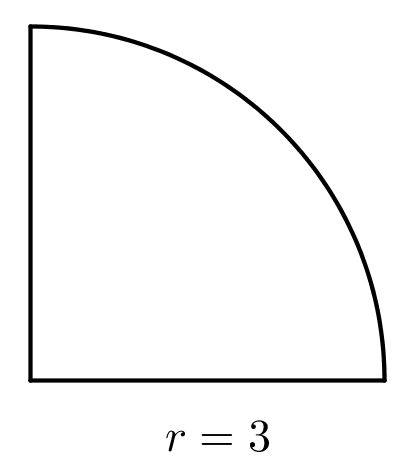
\includegraphics[width=0.3\textwidth]{pics/ViertelKreis}
        \end{center}
        } 
    \solution{$6+\frac{3}{2}\pi$}
\end{Add}

\begin{Add}{HaeK}{basal1.2}{Funktionen}{einfach}
    \question{
       Gib die Funktionsgleichung des Graphen an.
       \vspace{-0.2cm}
        \begin{center}
        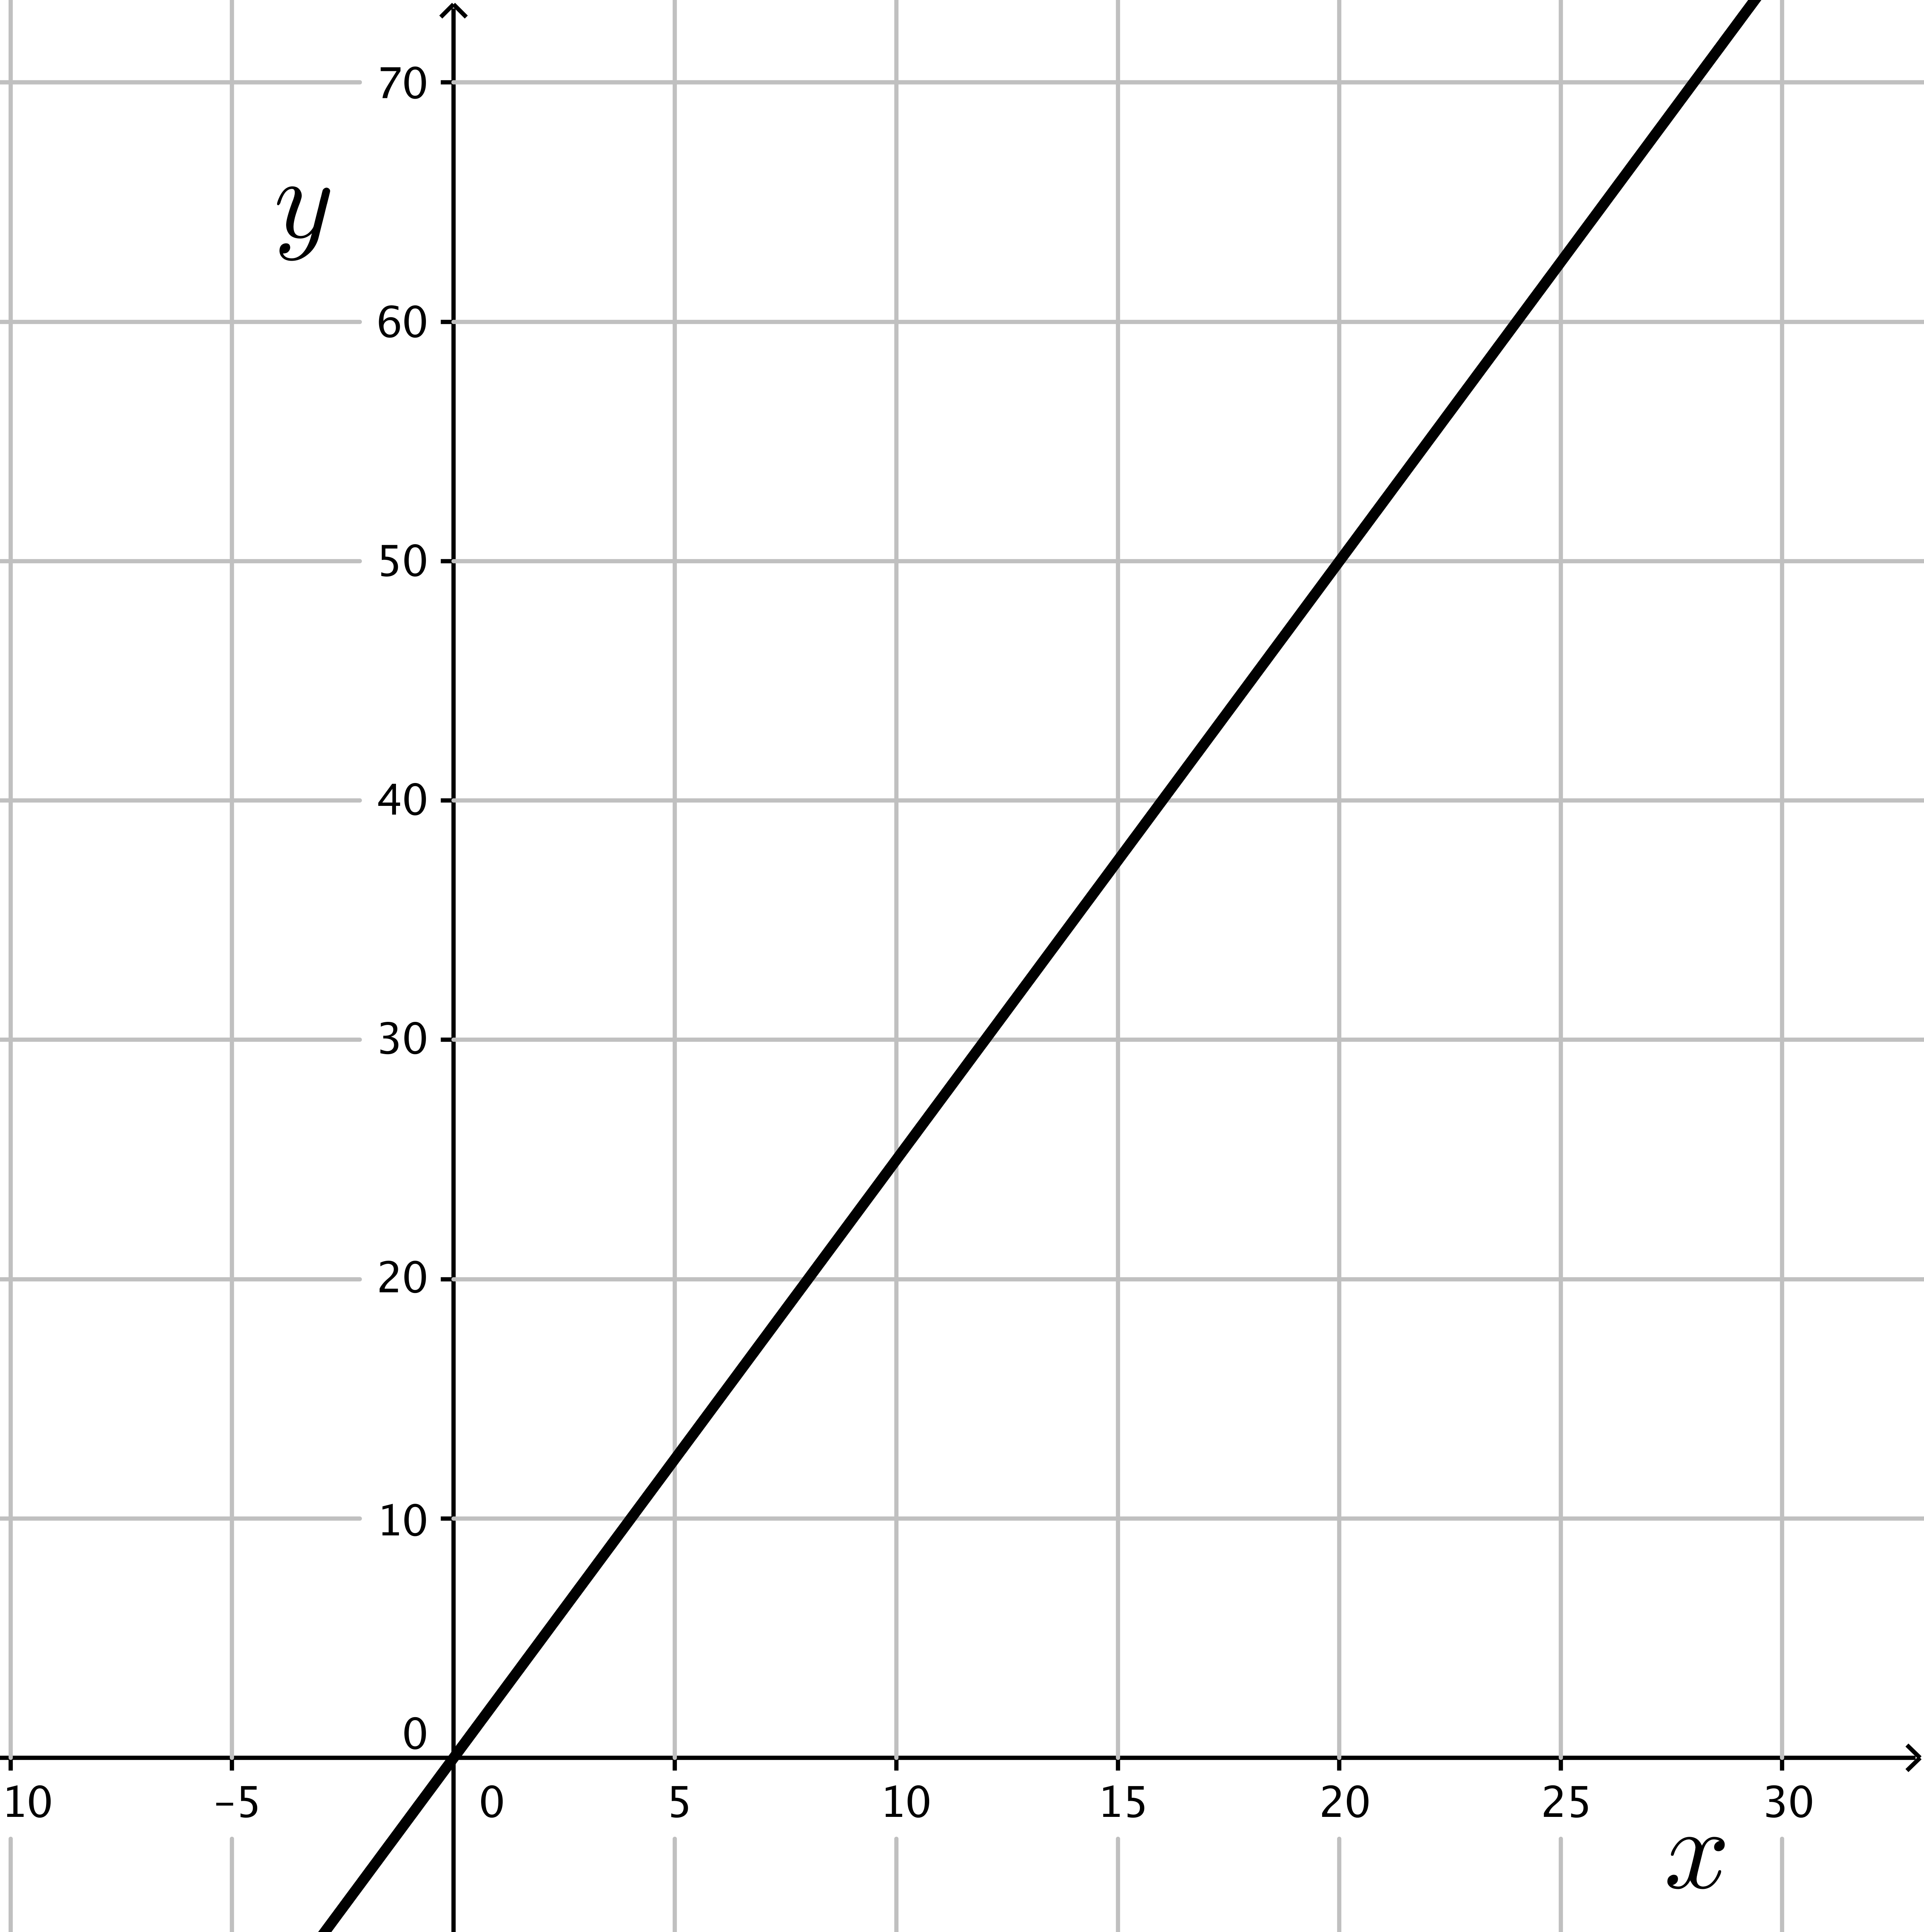
\includegraphics[width=0.45\textwidth]{pics/PropAchseSkal}
        \end{center}
        \vspace{-0.2cm}
        } 
    \solution{$y=2.5x$}
\end{Add}

\begin{Add}{HaeK}{basal1.2}{Geometrie}{schwieriger}
    \question{
       Stimmen diese Behauptungen? Begründe deine Antwort!
       \begin{enumerate}
       \item Alle Rechtecke sind zueinander ähnlich.
       \item Alle Quadrate sind zueinander ähnlich.
       \item Alle rechtwinkligen Dreiecke sind zueinander ähnlich.
       \end{enumerate}
     } 
    \solution{1. falsch 2. korrekt 3. falsch}
\end{Add}

\begin{Add}{HaeK}{basal1.2}{Geometrie}{einfach}
    \question{
       Berechne die fehlende Seite in der ähnlichen Figur. 
   \begin{center}
        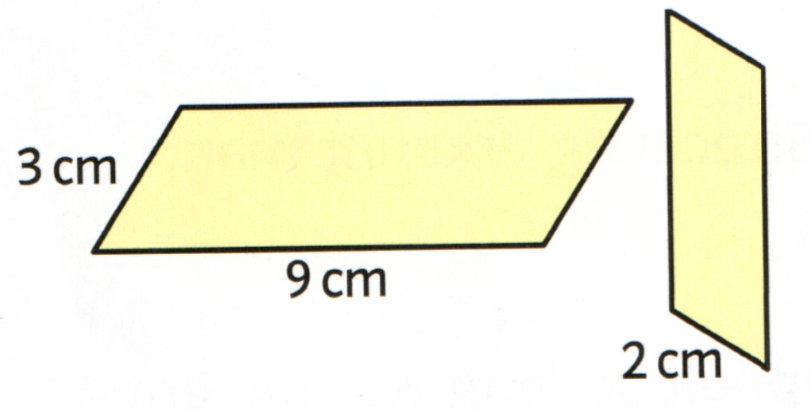
\includegraphics[width=0.45\textwidth]{pics/Aehnlich.png}
        \end{center}
     } 
    \solution{6cm}
\end{Add}

\begin{Add}{HaeK}{basal1.1}{Algebra,Bruchterme,Gleichungen}{einfach}
    \question{
      Löse die Gleichung nach $x$ auf.
    $$\dfrac{2x+1}{3}+\dfrac{2x-1}{4}=\dfrac{5}{4}$$
     } 
    \solution{1}
\end{Add}

\begin{Add}{HaeK}{basal1.1}{Koordinatensystem,Funktionen}{einfach}
    \question{
    Beschreibe, wie die Punktmenge, welche mit der Gleichung $x=0$ beschrieben wird, im Koordinatensystem aussieht. 
     } 
    \solution{Dies ist die $y$-Achse.}
\end{Add}

\begin{Add}{HaeK}{basal1.1}{Koordinatensystem,Funktionen}{einfach}
    \question{
    Beschreibe, wie die Punktmenge, welche mit der Gleichung $y=0$ beschrieben wird, im Koordinatensystem aussieht. 
     } 
    \solution{Dies ist die $x$-Achse.}
\end{Add}

\begin{Add}{HaeK}{basal1.1}{Sachrechnen}{einfach}
    \question{
    Wenn man $7\cdot 10^{19}$ km$^3$ in $7\cdot 10^{?}$ $\mu$m$^3$ umwandelt, ist ? dann grösser oder kleiner als 19?
     } 
    \solution{Viel grösser.}
\end{Add}

\begin{Add}{HaeK}{basal1.1}{Sachrechnen}{einfach}
    \question{
    Wenn man $3\cdot 10^{11}$ m$^3$ in $3\cdot 10^{?}$ km$^3$ umwandelt, ist ? dann grösser oder kleiner als 11?
     } 
    \solution{Kleiner.}
\end{Add}

\begin{Add}{HaeK}{basal1.1}{Sachrechnen}{einfach}
    \question{
    Wenn man $5\cdot 10^{22}$ Hz in $5\cdot 10^{?}$ GHz umwandelt, ist ? dann grösser oder kleiner als 22?
     } 
    \solution{Viel kleiner.}
\end{Add}

\begin{Add}{HaeK}{basal1.1}{Sachrechnen}{einfach}
    \question{
    Wenn man $7\cdot 10^{19}$ km$^3$ in $7\cdot 10^{?}$ $\mu$m$^3$ umwandelt, ist ? dann grösser oder kleiner als 19?
     } 
    \solution{Viel grösser.}
\end{Add}

\begin{Add}{HaeK}{basal1.2}{Funktionen}{schwieriger}
    \question{
   Welche der folgenden Funktionsgleichungen kann das Abschmelzen einer Kerze als Funktion der Anzünddauer $t$ beschreiben?
   $$f(t)=5t+10$$
   $$g(t)=-5t+10$$
   $$h(t)=-5t-10$$
   $$i(t)=5t-10$$
    } 
    \solution{g(t)}
\end{Add}

\begin{Add}{HaeK}{basal1.2}{Funktionen,Mathematisieren}{schwieriger}
    \question{
    Übersetze die Situation "Ein Stalagmit ist anfänglich 2m hoch und wächst in jedem Jahr um einen cm" in eine Funktion der Zeit (wobei die Zeit in Jahren gemesssen wird).
    } 
    \solution{$f(t)=2+0.01t$ (in Metern) oder $f(t)=200+t$ (in Zentimetern)}
\end{Add}

\begin{Add}{HaeK}{basal1.2}{Funktionen,Mathematisieren}{schwieriger}
    \question{Drücke die Aussage "Durch die Funktion $f$ wird der Zahl 2 die Zahl 78 zugeordnet" in mathematischer Schreibweise aus.} 
    \solution{$f(2)=78$}
\end{Add}


\begin{Add}{WiD}{basal0}{Geometrie,Arithmetik}{einfach}
    \question{
        Berechne in einem rechtwinkligen Dreieck die Kathete $a$ falls $b=4$ und $c=5$.
        \begin{center}
        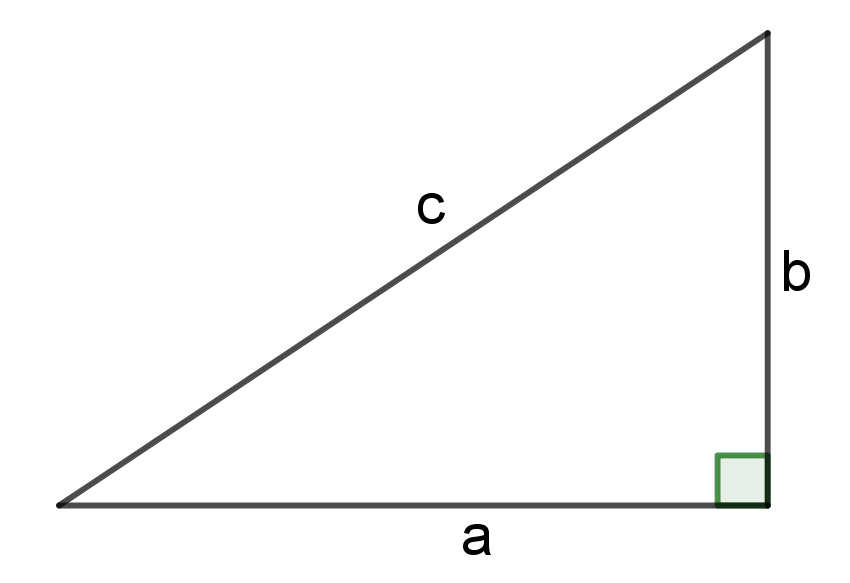
\includegraphics[width=0.5\textwidth]{pics/triangle}
        \end{center}
        } 
    \solution{$c^2=a^2+b^2 \rightarrow a=3$}
\end{Add}

\begin{Add}{WiD}{basal0}{Geometrie,Mathematisieren}{einfach}
    \question{
        In einem gleichschenkligen Dreieck misst der eine Basiswinkel $\alpha=37^{\circ}$. Berechne die restlichen Winkel im Dreieck. 
        } 
    \solution{$\alpha=\beta=37^{\circ} \rightarrow \gamma=180^{\circ}-2\cdot 37^{\circ}=106^{\circ}$}
\end{Add}

\begin{Add}{WiD}{basal1.2}{Geometrie}{schwieriger}
    \question{
        Was ist korrekt? \\
        Der Inkreismittelpunkt eines Dreiecks ist der Schnittpunkt der
        \begin{itemize}
            \item[a)] Seitenhalbierenden
            \item[b)] Mittelsenkrechten
            \item[c)] Winkelhalbierenden
            \item[d)] Höhenlinien
        \end{itemize}
        } 
    \solution{c)}
\end{Add}

\begin{Add}{WiD}{basal1.2}{Geometrie}{schwieriger}
    \question{
        In welchem Dreieck entspricht eine Schwerelinie gerade einer Winkelhalbierenden?
        } 
    \solution{In einem gleichschenkligen}
\end{Add}

\begin{Add}{WiD}{basal1.2}{Geometrie}{schwieriger}
    \question{
        In welchem Dreieck liegt der Umkreismittelpunkt auf einer Seite?
        } 
    \solution{In einem rechtwinkligen}
\end{Add}

\begin{Add}{WiD}{basal0}{Geometrie}{einfach}
    \question{
        Welche Aussagen über Rhomben sind korrekt? \\
        \begin{itemize}
            \item[a)] Im Rhombus halbieren sich die Diagonalen.
            \item[b)] Zwei gegenüberliegende Winkel ergänzen sich zu $180^{\circ}$.
            \item[c)] Ein Rhombus ist ein Rechteck.
            \item[d)] Gegenüberliegende Seiten sind parallel.
        \end{itemize}
        } 
    \solution{a), d)}
\end{Add}

\begin{Add}{WiD}{basal1.1}{Algebra,Bruchterme}{schwieriger}
    \question{
        Vereinfache soweit als möglich 
        $$\frac{1}{a-1}-\frac{a+1}{a^2-1}+\frac{1}{a}$$
        } 
    \solution{$\frac{1}{a}$}
\end{Add}

\begin{Add}{WiD}{basal0}{Geometrie,Koordinatensystem}{einfach}
    \question{
        Spiegle den Punkt $A=(2;5)$ an der \begin{itemize}
            \item[a)] $x$-Achse 
            \item[b)] $y$- Achse
        \end{itemize}
        } 
    \solution{a) $A'=(2;-5)$ \quad b) $A''=(-2;5)$}
\end{Add}

\begin{Add}{WiD}{basal1.2}{Geometrie,Koordinatensystem}{schwieriger}
    \question{
        Spiegle den Punkt $A=(-2;5)$ am Punkt $S=(1;4)$
        } 
    \solution{$A'=(4;3)$}
\end{Add}

\begin{Add}{WiD}{basal1.1}{Koordinatensystem,Geometrie}{schwieriger}
    \question{
        Spannen die vier Punkte $A=(-9;3)$, $B=(-5;-3)$, $C=(1;1)$ und $D=(-3;7)$ ein Quadrat auf? Warum?
        } 
    \solution{Ja, denn sowohl die Seitenlängen ($\sqrt{52}$) als auch die Diagonalen ($\sqrt{104}$) sind gleich lang}
\end{Add}

\begin{Add}{WiD}{basal1.1}{Bruchterme,Arithmetik}{einfach}
    \question{
        Welcher Bruch ist kleiner? (Ohne 
        Taschenrechner!)
        \[ \dfrac{13}{17} \quad \text{ oder } \quad \dfrac{3}{4} \]
        } 
    \solution{$\frac{3}{4}$}
\end{Add}

\begin{Add}{WiD}{basal0}{Algebra,Grundoperationen}{einfach}
    \question{
        Vereinfache soweit als möglich:
        \[ 3x-6y-2(1+4x-3y) \]
        } 
    \solution{$-2-5x$}
\end{Add}

\begin{Add}{WiD}{basal1.1}{Algebra,Grundoperationen}{schwieriger}
    \question{
        Vereinfache soweit als möglich:
        \[ 15a-\big((3a-6b)-c\big)-\big((5b-(-10a+4c)\big) \]
        } 
    \solution{$2a+b+5c$}
\end{Add}

\begin{Add}{WiD}{basal1.1}{Algebra,Grundoperationen}{schwieriger}
    \question{
        Vereinfache soweit als möglich:
        \[ -3(-2u)^3(1.5u)^2(-u)^4 \]
        } 
    \solution{$54u^9$}
\end{Add}

\begin{Add}{WiD}{basal0}{Algebra,Grundoperationen}{einfach}
    \question{
        Multipliziere aus:
        \[ (a+b)(1+a-b) \]
        } 
    \solution{$a^2+a+b-b^2$}
\end{Add}

\begin{Add}{WiD}{basal1.1}{Algebra,Grundoperationen}{einfach}
    \question{
        Multipliziere aus:
        \[ (a^2+1)(a^2-a-1) \]
        } 
    \solution{$a^4-a^3-a-1$}
\end{Add}

\begin{Add}{WiD}{basal1.1}{Algebra,Gleichungen,Lineares}{einfach}
    \question{
        Welcher Term muss im Kasten \framebox[10mm]{\rule{0mm}{3mm}} stehen, damit die Gleichung erfüllt ist?
        \[ 3x+4y-\framebox[10mm]{\rule{0mm}{3mm}}=x-y \]
        } 
    \solution{$2x+5y$}
\end{Add}

\begin{Add}{WiD}{basal1.1}{Algebra,Gleichungen,Bruchterme}{schwieriger}
    \question{
        Welcher Term muss im Kasten \framebox[10mm]{\rule{0mm}{3mm}} stehen, damit die Gleichung erfüllt ist?
        \[ \frac{5a}{\framebox[10mm]{\rule{0mm}{3mm}}}=\frac{1}{b} \]
        } 
    \solution{$5ab$}
\end{Add}

\begin{Add}{WiD}{basal1.1}{Algebra,Gleichungen,Bruchterme}{schwieriger}
    \question{
        Welcher Term muss im Kasten \framebox[10mm]{\rule{0mm}{3mm}} stehen, damit die Gleichung erfüllt ist?
        \[ -\frac{\framebox[10mm]{\rule{0mm}{3mm}}}{a}=a \]
        } 
    \solution{$-a^2$}
\end{Add}

\begin{Add}{WiD}{basal0}{Arithmetik,Sachrechnen}{einfach}
    \question{
        Wie viel sind 30\% von 60\%? 
        \begin{itemize}
            \item[a)] 30\%
            \item[b)] 50\%
            \item[c)] 18\%
            \item[d)] 2\%
        \end{itemize}
        } 
    \solution{c)}
\end{Add}

\begin{Add}{WiD}{basal0}{Arithmetik,Bruchterme,Grundoperationen}{einfach}
    \question{
        Berechne mit dem Taschenrechner und runde auf 4 signifikante Stellen: 
        \[ -\frac{1}{\frac{2}{3}-\frac{1}{5}} \]
        } 
    \solution{$2.143$}
\end{Add}

\begin{Add}{WiD}{basal0}{Arithmetik,Bruchterme,Grundoperationen}{einfach}
    \question{
        Berechne mit dem Taschenrechner und runde auf 4 signifikante Stellen: 
        \[ \tfrac{1}{7}-(\tfrac{3}{8}-1) \]
        } 
    \solution{$0.7679$}
\end{Add}

\begin{Add}{WiD}{basal0}{Arithmetik,Bruchterme,Wurzelterme,Grundoperationen}{einfach}
    \question{
        Berechne mit dem Taschenrechner und runde auf 4 signifikante Stellen: 
        \[ 2-2\sqrt{1-\tfrac{1}{3}} \]
        } 
    \solution{$0.3670$}
\end{Add}

\begin{Add}{WiD}{basal0}{Arithmetik,Bruchterme,Wurzelterme,Grundoperationen}{schwieriger}
    \question{
        Berechne mit dem Taschenrechner und runde auf 4 signifikante Stellen: 
        \[ \frac{1-\tfrac{11}{9}}{\sqrt{3}+2} \]
        } 
    \solution{$-0.05954$}
\end{Add}

\begin{Add}{WiD}{basal0}{Arithmetik,Bruchterme,Grundoperationen}{einfach}
    \question{
        Berechne mit dem Taschenrechner und runde auf 4 signifikante Stellen: 
        \[ 1-\frac{1}{3}\left(1-\frac{1}{3}\Big(1-\tfrac{1}{3}(1-\tfrac{1}{3})\Big)\right) \]
        } 
    \solution{$0.7531$}
\end{Add}

\begin{Add}{WiD}{basal1.1}{Algebra,Bruchterme,Grundoperationen}{schwieriger}
    \question{
        Vereinfache soweit als möglich: 
        \[ a-\tfrac{1}{2}b+2\left(\tfrac{3}{4}b-\tfrac{2}{5}a\right)-\frac{a-b}{2} \]
        } 
    \solution{$\frac{6}{5}b$}
\end{Add}

\begin{Add}{WiD}{basal0}{Algebra,Bruchterme,Grundoperationen}{einfach}
    \question{
        Vereinfache soweit als möglich: 
        \[ \frac{-2\cdot3ab}{-4b} \]
        } 
    \solution{$\frac{3}{2}a$}
\end{Add}

\begin{Add}{WiD}{basal0}{Algebra,Bruchterme,Grundoperationen}{einfach}
    \question{
        Vereinfache soweit als möglich: 
        \[ -\frac{2\cdot3ab}{-4b} \]
        } 
    \solution{$\frac{3}{2}a$}
\end{Add}

\begin{Add}{WiD}{basal0}{Algebra,Bruchterme,Grundoperationen}{einfach}
    \question{
        Vereinfache soweit als möglich: 
        \[ -\frac{-2\cdot3ab}{4b} \]
        } 
    \solution{$\frac{3}{2}a$}
\end{Add}

\begin{Add}{WiD}{basal1.1}{Arithmetik,Wurzelterme}{schwieriger}
    \question{
        Welche Gleichungen sind wahr? 
        \begin{itemize}
            \item[a)] $\sqrt{49}=-7$
            \item[b)] $\sqrt{144+25}=\sqrt{144}+\sqrt{25}$
            \item[c)] $\sqrt{36\cdot81}=\sqrt{36}\cdot\sqrt{81}$
            \item[d)] $\sqrt{\frac{64}{121}}=\frac{\sqrt{64}}{\sqrt{81}}$
        \end{itemize}
        } 
    \solution{c) und d)}
\end{Add}

\begin{Add}{WiD}{basal0}{Sachrechnen,Arithmetik}{einfach}
    \question{
        Wie viel sind 90\% von 20\%?
        } 
    \solution{$18\%$}
\end{Add}

\begin{Add}{WiD}{basal1.1}{Sachrechnen,Mathematisieren}{schwieriger}
    \question{
        Der Preis einer Hose wird um 10\% reduziert und anschliessend um 11\% erhöht. Ist sie jetzt teurer, billiger oder gleich teuer wie zu Beginn?
        } 
    \solution{billiger}
\end{Add}


\begin{Add}{WaJ}{basal1.1}{Arithmetik}{einfach}
    \question{
        $$2\cdot10^5\cdot7\cdot10^9=\;?$$
    }
    \solution{
        $14\cdot10^{14}=1.4\cdot10^{15}$
    }
\end{Add}

\begin{Add}{WaJ}{basal0}{Bruchterme}{schwieriger}
    \question{
        $$\frac{2}{3}-\frac{5}{7}=\;?$$
    }
    \solution{
        $-\frac{1}{21}$
    }
\end{Add}

\begin{Add}{WaJ}{basal1.1}{Arithmetik}{einfach}
    \question{
        $$\sqrt{4\cdot10^{12}}=\;?$$
    }
    \solution{
        $2\cdot10^6$
    }
\end{Add}

\begin{Add}{WaJ}{basal1.2}{Algebra}{schwieriger}
    \question{
        $$\frac{2x}{\frac{4x}{5}}=\;?$$
    }
    \solution{
        $\frac{5}{2}$
    }
\end{Add}

\begin{Add}{WaJ}{basal1.2}{Gleichungen}{schwieriger}
    \question{
        Löse nach $x$:
        $$-\frac{3}{7}x+5=2$$
    }
    \solution{
        $x=7$
    }
\end{Add}

\begin{Add}{WaJ}{basal1.1}{Sachrechnen}{schwieriger}
    \question{
        $$\unitfrac[72]{km}{h}=\unitfrac[\;?]{m}{s}$$
    }
    \solution{
        $\unitfrac[20]{m}{s}$
    }
\end{Add}

\begin{Add}{WaJ}{basal1.1}{Sachrechnen}{einfach}
    \question{
        $$\unitfrac[36]{km}{h}=\unitfrac[\;?]{m}{s}$$
    }
    \solution{
        $\unitfrac[10]{m}{s}$
    }
\end{Add}

\begin{Add}{WaJ}{basal1.1}{Sachrechnen}{einfach}
    \question{
        $$\unitfrac[10]{m}{s}=\unitfrac[\;?]{km}{h}=$$
    }
    \solution{
        $\unitfrac[36]{m}{s}$
    }
\end{Add}

\begin{Add}{WaJ}{basal0}{Sachrechnen}{einfach}
    \question{
        Wie viel Liter Wasser entsprechen dem Volumen eines Würfels mit Kantenlänge $\unit[1]{m}$?
    }
    \solution{
        $\unit[1000]{Liter}$
    }
\end{Add}

\begin{Add}{WaJ}{basal0}{Sachrechnen}{einfach}
    \question{
        Welches Volumen nehmen $\unit[1000]{Liter}$ Wasser ein?
    }
    \solution{
        $\unit[1]{m^3}$
    }
\end{Add}

\begin{Add}{WaJ}{basal1.2}{Sachrechnen}{einfach}
    \question{
        Wenn man die Kantenlägen eines Würfels verdoppelt, um wie viel nimmt
        \begin{enumerate}
            \item[a)] sein Volumen
            \item[b)] seine Oberfläche
        \end{enumerate}
        zu?
    }
    \solution{
        \begin{enumerate}
            \item[a)] um das 8-fache
            \item[b)] um das 4-fache
        \end{enumerate}
    }
\end{Add}

\begin{Add}{WaJ}{basal0}{Sachrechnen}{schwieriger}
    \question{
        Wenn man das Volumen einer Pyramide 27 mal grösser macht, um wie viel hat dann ihre Oberfläche zugenommen?
    }
    \solution{
        um das $9$-fache
    }
\end{Add}

\begin{Add}{WaJ}{basal0}{Sachrechnen}{schwieriger}
    \question{
        Wenn man die Oberfläche eines Quaders um den Faktor $16$ vergrössert, um wie viel nimmt dann sein Volumen zu?
    }
    \solution{
        um den Faktor $64$
    }
\end{Add}

\begin{Add}{WaJ}{basal1.1}{Sachrechnen}{schwieriger}
    \question{
        $$\unit[200]{Liter}=\unit[\;?]{m^3}$$
    }
    \solution{
        $\unit[0.2]{m^3}$
    }
\end{Add}

\begin{Add}{WaJ}{basal1.2}{Funktionen}{schwieriger}
    \question{
        Sei $f(x)=\frac{1}{2}x-1$. Bestimme
        $$f(-3)$$
    }
    \solution{
        $f(-3)=-\frac{5}{2}$
    }
\end{Add}

\begin{Add}{WaJ}{basal1.2}{Funktionen}{schwieriger}
    \question{
        Sei $f(x)=x^2$. Bestimme
        $$f(-2)$$
    }
    \solution{
        $f(-2)=4$
    }
\end{Add}

\begin{Add}{WaJ}{basal1.1}{Algebra,Grundoperationen}{einfach}
    \question{
        Faktorisiere
        $$x^2-2x+1$$
    }
    \solution{
        $(x-1)^2$
    }
\end{Add}

\begin{Add}{WaJ}{basal1.1}{Algebra,Grundoperationen}{schwieriger}
    \question{
        $$\left(2-\sqrt{2}\right)\left(2+\sqrt{2}\right)=\;?$$
    }
    \solution{
        $2$
    }
\end{Add}

\begin{Add}{WaJ}{basal1.1}{Geometrie,Grundoperationen}{schwieriger}
    \question{
        Gegeben seien die Katheten $a=\unit[4]{m}$ und $b=\unit[3]{m}$. 
        Wie lang ist die Seite $c$?
        \begin{center}
        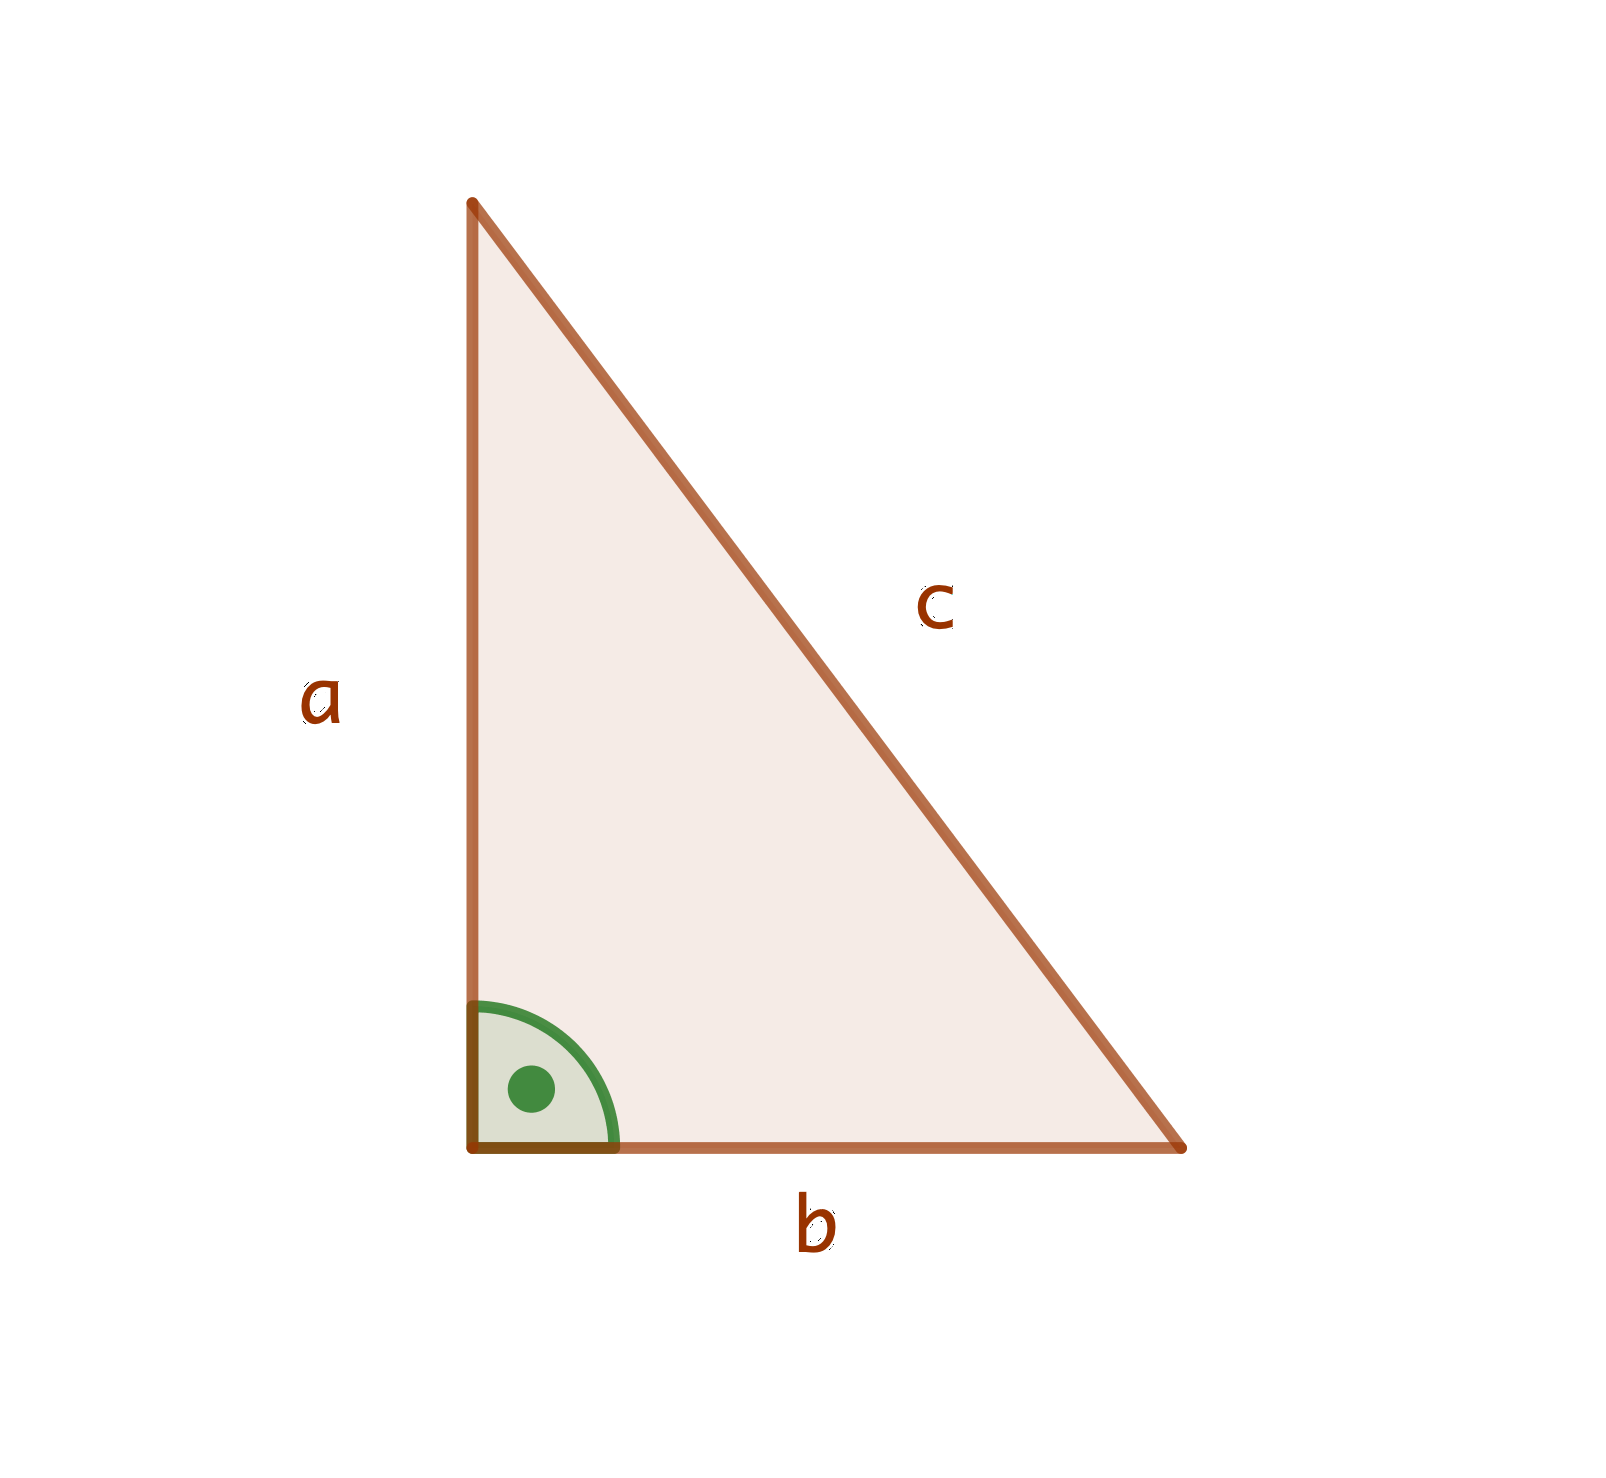
\includegraphics[width=0.382\textwidth]{pics/wajpythagoras.png}
        \end{center}
    }
    \solution{
        $c=\unit[5]{m}$
    }
\end{Add}

\begin{Add}{WaJ}{basal1.1}{Geometrie,Grundoperationen}{schwieriger}
    \question{
        Gegeben seien die Kathete $a=\unit[4]{m}$ und die Hypotenuse $c=\unit[5]{m}$. 
        Wie lang ist die Seite $b$?
        \begin{center}
        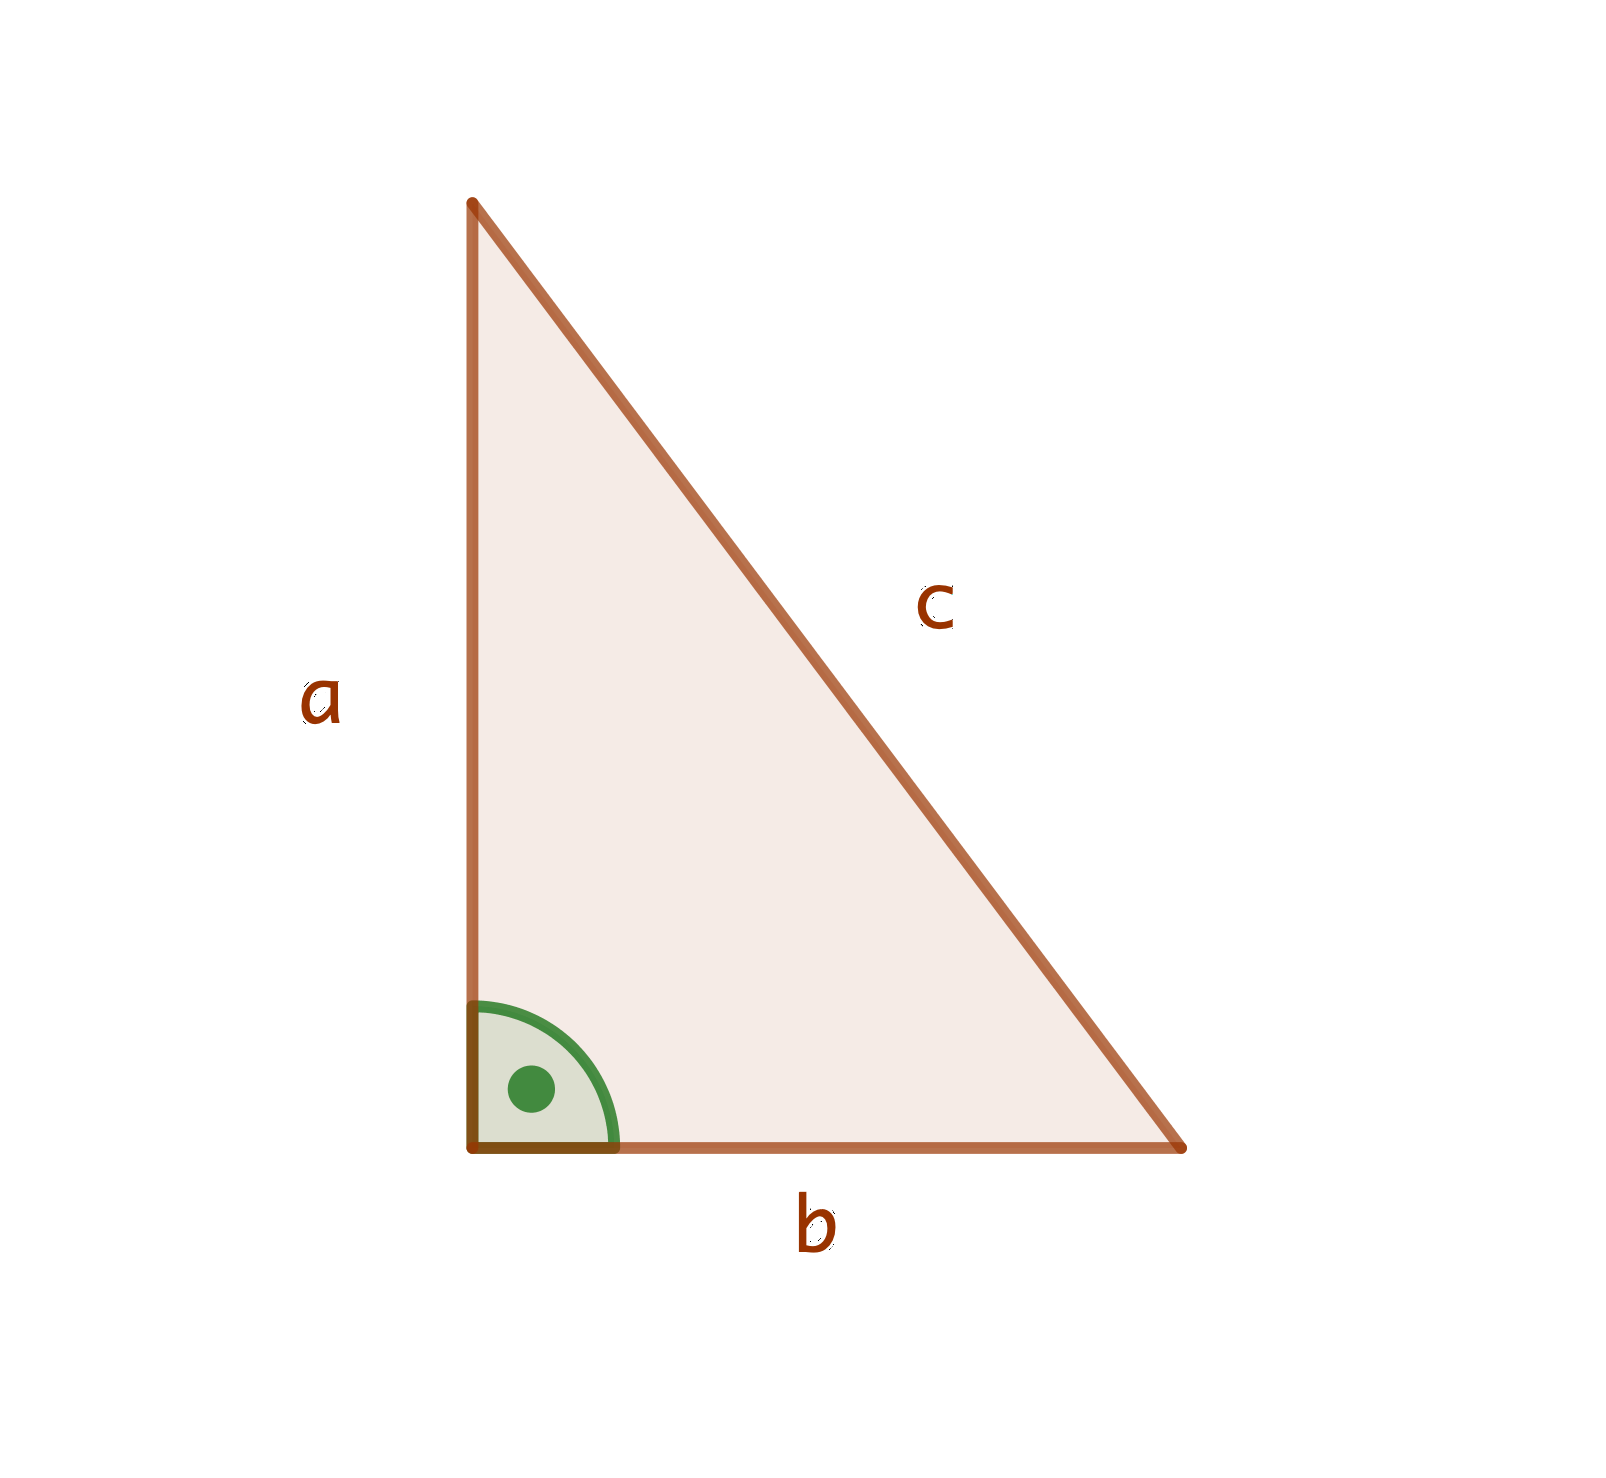
\includegraphics[width=0.382\textwidth]{pics/wajpythagoras.png}
        \end{center}
    }
    \solution{
        $c=\unit[3]{m}$
    }
\end{Add}

\begin{Add}{WaJ}{basal1.1}{Sachrechnen}{einfach}
    \question{
        Wie viel sind $\unit[80]{\%}$ von $\unit[80]{\%}$ von $200$.
    }
    \solution{
        $128$
    }
\end{Add}

\begin{Add}{WaJ}{basal1.1}{Geometrie}{schwieriger}
    \question{
        Wie lang ist der Umfang eines Kreises mit Radius $\unit[2]{m}$?
    }
    \solution{
        $\unit[4\pi]{m}$
    }
\end{Add}

\begin{Add}{WaJ}{basal1.1}{Geometrie}{einfach}
    \question{
        Wie gross ist die Fläche eines Kreises mit Radius $\unit[2]{m}$?
    }
    \solution{
        $\unit[4\pi]{m^2}$
    }
\end{Add}

\begin{Add}{WaJ}{basal1.1}{Geometrie}{schwieriger}
    \question{
        Wie gross ist die Fläche eines Kreises mit Durchmesser $\unit[1.6]{m}$?
    }
    \solution{
        $\unit[\frac{16}{25}\pi]{m^2}$
    }
\end{Add}

\begin{Add}{WaJ}{basal1.1}{Geometrie}{schwieriger}
    \question{
        Wie gross ist der Durchmesser eines Kreises mit Flä\-chen\-in\-halt $\unit[\frac{9\pi}{4}]{m^2}$?
    }
    \solution{
        $\unit[3]{m}$
    }
\end{Add}

\begin{Add}{WaJ}{basal1.1}{Algebra}{einfach}
    \question{
        $$2a-(4+a)=\;?$$
    }
    \solution{
        $a-4$
    }
\end{Add}

\begin{Add}{WaJ}{basal1.1}{Algebra}{schwieriger}
    \question{
        $$2a-(4+a)\cdot(-2)=\;?$$
    }
    \solution{
        $4(a+2)=4a+8$
    }
\end{Add}

\begin{Add}{WaJ}{basal1.1}{Arithmetik,Grundoperationen}{einfach}
    \question{
        $$(-2)\cdot(-3)^2=\;?$$
    }
    \solution{
        $-18$
    }
\end{Add}

\begin{Add}{WaJ}{basal1.1}{Algebra}{einfach}
    \question{
        $$xy+x+y-yx=\;?$$
    }
    \solution{
        $x+y$
    }
\end{Add}

\begin{Add}{WaJ}{basal0}{Arithmetik}{einfach}
    \question{
        $$3-\frac{7}{5}=\;?$$
    }
    \solution{
        $\frac{8}{5}$
    }
\end{Add}

\begin{Add}{WaJ}{basal0}{Arithmetik}{schwieriger}
    \question{
        $$\left(1-3\cdot\left(-\frac{7}{6}\right)\right)^2=\;?$$
    }
    \solution{
        $\frac{81}{4}$
    }
\end{Add}

\begin{Add}{WaJ}{basal0}{Arithmetik}{einfach}
    \question{
        $$\frac{2}{3}+\frac{2}{3}=\;?$$
    }
    \solution{
        $\frac{4}{3}$
    }
\end{Add}

\begin{Add}{WaJ}{basal1.2}{Gleichungen}{schwieriger}
    \question{
        $$\frac{1}{2}+\frac{1}{3}+x=1$$
    }
    \solution{
        $\frac{1}{6}$
    }
\end{Add}

\begin{Add}{WaJ}{basal1.2}{Gleichungen}{einfach}
    \question{
        $$\frac{5}{7}\cdot x=1$$
    }
    \solution{
        $\frac{7}{5}$
    }
\end{Add}

\begin{Add}{WaJ}{basal1.2}{Gleichungen}{einfach}
    \question{
        $$\frac{5}{7}\div x=1$$
    }
    \solution{
        $\frac{5}{7}$
    }
\end{Add}

\begin{Add}{WaJ}{basal1.2}{Gleichungen}{einfach}
    \question{
        $$\frac{5}{7}+x=1$$
    }
    \solution{
        $\frac{2}{7}$
    }
\end{Add}

\begin{Add}{WaJ}{basal1.2}{Gleichungen}{einfach}
    \question{
        $$\frac{5}{7}-x=1$$
    }
    \solution{
        $-\frac{2}{7}$
    }
\end{Add}

\begin{Add}{WaJ}{basal0}{Arithmetik}{einfach}
    \question{
        $$\frac{2}{3}+\frac{3}{2}=\;?$$
    }
    \solution{
        $\frac{13}{6}$
    }
\end{Add}

\begin{Add}{WaJ}{basal0}{Arithmetik}{einfach}
    \question{
        $$\frac{2}{-3}+\frac{3}{2}\cdot\frac{4}{9}=\;?$$
    }
    \solution{
        $0$
    }
\end{Add}

\begin{Add}{WaJ}{basal0}{Arithmetik}{schwieriger}
    \question{
        $$\frac{\frac{4}{3}}{\frac{1}{2}}-\frac{3}{7}\cdot\frac{35}{9}=\;?$$
    }
    \solution{
        $1$
    }
\end{Add}

\begin{Add}{WaJ}{basal0}{Algebra}{schwieriger}
    \question{
    Wahr oder falsch?
        $$\frac{a}{-b}=-\frac{a}{b}=\frac{-a}{b}$$
    }
    \solution{
        wahr
    }
\end{Add}

\begin{Add}{WaJ}{basal0}{Arithmetik}{einfach}
    \question{
    Wahr oder falsch?
        $$\frac{1}{-2}=-\frac{1}{2}=\frac{-1}{2}$$
    }
    \solution{
        wahr
    }
\end{Add}

\begin{Add}{WaJ}{basal0}{Arithmetik}{einfach}
    \question{
    Wahr oder falsch?
        $$\frac{1}{-3^2}=-\frac{1}{3^2}=\frac{-1^2}{3^2}$$
    }
    \solution{
        wahr
    }
\end{Add}

\begin{Add}{WaJ}{basal0}{Arithmetik}{einfach}
    \question{
    Wahr oder falsch?
        $$-\frac{1}{2}^2=\left(-\frac{1}{2}\right)^2$$
    }
    \solution{
        falsch
    }
\end{Add}

\begin{Add}{WaJ}{basal0}{Arithmetik}{einfach}
    \question{
    Wahr oder falsch?
        $$-\frac{1^2}{2^2}=\left(-\frac{1}{2}\right)^2$$
    }
    \solution{
        falsch
    }
\end{Add}

\begin{Add}{WaJ}{basal0}{Arithmetik}{schwieriger}
    \question{
    Wahr oder falsch?
        $$\frac{-1^3}{-2^3}=\left(-\frac{1}{2}\right)^3$$
    }
    \solution{
        falsch
    }
\end{Add}

\begin{Add}{WaJ}{basal0}{Arithmetik,Grundoperationen}{einfach}
    \question{
        $$4-2^4\cdot3=\;?$$
    }
    \solution{
        $-44$
    }
\end{Add}

\begin{Add}{WaJ}{basal0}{Arithmetik,Grundoperationen}{einfach}
    \question{
        $$4-3\cdot(-2)^3=\;?$$
    }
    \solution{
        $28$
    }
\end{Add}

\begin{Add}{WaJ}{basal1.1}{Algebra,Gleichungen}{schwieriger}
    \question{
        $$4+3\cdot x^3=\;28$$
    }
    \solution{
        $2$
    }
\end{Add}

\begin{Add}{WaJ}{basal1.1}{Arithmetik}{einfach}
    \question{
        $$36-4\cdot 2^3=\;?$$
    }
    \solution{
        $4$
    }
\end{Add}

\begin{Add}{WaJ}{basal0}{Geometrie}{einfach}
    \question{
        In einem gleichseitigen Dreieck betragen die Winkel \dots$^\circ$
    }
    \solution{
        $60^\circ$
    }
\end{Add}

\begin{Add}{WaJ}{basal0}{Geometrie}{einfach}
    \question{
        In einem rechtwinkligen, gleichschenkligen Dreieck betragen die Basiswinkel \dots$^\circ$
    }
    \solution{
        $45^\circ$
    }
\end{Add}

\begin{Add}{WaJ}{basal0}{Geometrie}{schwieriger}
    \question{
        In einem gleichschenkligen, rechtwinkligen Dreieck mit Kathetenlängen jeweils $1$ beträgt die Hypotenuse \dots
    }
    \solution{
        $\sqrt{2}$
    }
\end{Add}

\begin{Add}{WaJ}{basal0}{Geometrie}{einfach}
    \question{
        Wenn in einem rechtwinkligen Dreieck die Hypotenuse $3$ und eine Kathete $2$ lang ist, dann ist die andere Kathete \dots\ lang.
    }
    \solution{
        $\sqrt{5}$
    }
\end{Add}

\begin{Add}{WaJ}{basal0}{Geometrie}{schwieriger}
    \question{
        In einem gleichseitigen Dreieck betrage die Höhe $\sqrt{3}$. Wie lang ist eine Seite?
    }
    \solution{
        $2$
    }
\end{Add}


\begin{Add}{RoK}{basal0}{Arithmetik,Geometrie,Mathematisieren}{schwieriger}
    \question{
        Die drei Innenwinkel eines Dreiecks verhalten sich wie $3:4:5$. Wie gross sind die drei Winkel?
    }
    \solution{
        $45^\circ$, $60^\circ$ und $75^\circ$
    }
\end{Add}


% Basal (HaeK)?
\begin{Add}{RoK}{basal1.1}{Mathematisieren,Gleichungen,Lineares}{schwieriger}
    \question{
        Wird auf beiden Seiten einer zweistelligen natürlichen Zahl die Ziffer 5 hinzugefügt, so ergibt sich das 75-fache der Zahl.\\
        Erkläre die folgende Gleichung:
        $$5000+10x+5=75x$$
    }
    \solution{
        $+5$: Ziffer 5 rechts hinzufügen. $10x$: ...zweistellige Zahl wird so eine Stelle nach links verschoben. $+5000$: Ziffer 5 links hinzufügen. $=75x$: Neue Zahl entspricht dem 75-fachen des Originals.
    }
\end{Add}

\begin{Add}{RoK}{basal1.1}{Algebra}{schwieriger}
    \question{
        Löse die Gleichung nach $x$ auf:
        $$5^x=5\cdot 5^{20}+20\cdot 5^{20}$$
    }
    \solution{
        $x=22$
    }
\end{Add}

\begin{Add}{RoK}{basal1.1}{Algebra}{schwieriger}
    \question{
        Löse die Gleichung nach $x$ auf:
        $$2\cdot 4^x-24\cdot 4^{32}=8\cdot 4^{32}$$
    }
    \solution{
        $x=34$
    }
\end{Add}

\begin{Add}{RoK}{basal0}{Arithmetik,Grundoperationen}{einfach}
    \question{
        Welche Zahl liegt auf der Zahlengerade exakt zwischen $-\frac{2}{3}$ und $\frac{1}{5}$?
    }
    \solution{
        $-\frac{7}{30}$
    }
\end{Add}

\begin{Add}{RoK}{basal0}{Arithmetik}{einfach}
    \question{
        Berechne das kgV und den ggT der Zahlen 14 und 35.
    }
    \solution{
        $kgV(14,35)=70,~ggT(14,35)=7$
    }
\end{Add}

\begin{Add}{RoK}{basal0}{Mathematisieren,Algebra}{einfach}
    \question{
        Der Term ist ein Quotient. Der Dividend ist die Differenz aus $x$ und $y$, der Divisor ist die Summe aus 2 und $z$. Wie lautet der Term?
    }
    \solution{
        $\frac{x-y}{2+z}$
    }
\end{Add}

\begin{Add}{RoK}{basal0}{Arithmetik}{einfach}
    \question{
        Berechne das kgV und den ggT der Zahlen 45 und 75.
    }
    \solution{
        $kgV(14,35)=225,~ggT(14,35)=15$
    }
\end{Add}

% Eher anspruchsvoll (HaeK)
\begin{Add}{RoK}{basal1.1}{Grundoperationen,Arithmetik,Wurzelterme}{schwieriger}
    \question{
        Ordne nach aufsteigender Grösse:
        $$\pi,~\frac{16}{5},~\sqrt{13},~2^2,~\frac{28}{9},~\sqrt{\sqrt{81}}$$
    }
    \solution{
        $\sqrt{\sqrt{81}},~\frac{28}{9},~\pi,~\frac{16}{5},~\sqrt{13},~2^2$
    }
\end{Add}

\begin{Add}{RoK}{basal0}{Sachrechnen,Arithmetik}{einfach}
    \question{
        $20~m^2$ entsprechen $2\cdot 10^x~mm^2$. 
    }
    \solution{
        $x=7$
    }
\end{Add}

\begin{Add}{RoK}{basal0}{Sachrechnen,Arithmetik}{einfach}
    \question{
        Auf einem Fussballfeld mit den Massen 100 mal 50 Meter steht das Wasser 1 cm hoch. Wie viele Liter Wasser sind das? 
    }
    \solution{
        50'000 Liter
    }
\end{Add}

\begin{Add}{RoK}{basal0}{Sachrechnen,Arithmetik}{einfach}
    \question{
        Ein Aquarium hat eine Breite von 80 cm, eine Tiefe von 40 cm und eine Höhe von 50 cm. Wie viele Liter passen maximal in das Aquarium? 
    }
    \solution{
        160 Liter
    }
\end{Add}

\begin{Add}{RoK}{basal0}{Sachrechnen,Arithmetik}{einfach}
    \question{
        Ein Quader mit quadratischer Grundfläche und der Höhe 40 cm soll ein Volumen von einem Liter haben. Welche Masse hat die Grundfläche? 
    }
    \solution{
        Das Grundquadrat hat eine Seitenlänge von 5 cm
    }
\end{Add}

\begin{Add}{RoK}{basal1.1}{Algebra,Lineares}{schwieriger}
    \question{
        $$\frac{10+x}{18}=\frac{10-x}{12}$$
    }
    \solution{
        $x=2$
    }
\end{Add}

\begin{Add}{RoK}{basal0}{Arithmetik}{einfach}
    \question{
        $$\frac{1}{1}+\frac{1}{2}+\frac{1}{3}+\frac{1}{4}=$$
    }
    \solution{
        $\frac{25}{12}$
    }
\end{Add}

% Ohne TR IMO klar nicht basal (haben ursprünglich gesagt, dass alle Rechnungen - sofern nicht anders deklariert- ohne TR sind)

\begin{Add}{RoK}{basal0}{Geometrie,Lineares}{einfach}
    \question{
        Ein Velorad hat einen Durchmesser von 28 Zoll. Ein Zoll entspricht 2.54 cm. Durch welche Rechnung kannst du ermitteln, wie weit das Velo mit einer Radumdrehung fährt?
    }
    \solution{
        $28\cdot 2.54\cdot 2\cdot\pi$ cm
    }
\end{Add}

\begin{Add}{RoK}{basal0}{Arithmetik}{einfach}
    \question{
        Berechne den Kehrwert von $\frac{1}{3}-\frac{1}{4}$.
    }
    \solution{
        12
    }
\end{Add}

\begin{Add}{RoK}{basal0}{Arithmetik}{einfach}
    \question{
        Welcher Bruch ist grösser, $\frac{2}{3}$ oder $\frac{11}{16}$?
    }
    \solution{
        $\frac{11}{16}$
    }
\end{Add}

\begin{Add}{RoK}{basal0}{Arithmetik,Wurzelterme}{einfach}
    \question{
        Berechne $x=\sqrt{13^2-3^2-12^2}$.
    }
    \solution{
        $x=4$
    }
\end{Add}

\begin{Add}{RoK}{basal0}{Arithmetik,Grundoperationen}{einfach}
    \question{
        Setze ein paar Klammern so, dass der folgende Ausdruck möglichst gross wird.\\
        $$2\cdot 3+4^2$$
    }
    \solution{
        $(2\cdot 3+4)^2$
    }
\end{Add}

\begin{Add}{RoK}{basal0}{Arithmetik,Grundoperationen}{einfach}
    \question{
        Vereinfache.\\
        $$a\cdot a\cdot a+a\cdot a\cdot a\cdot a$$
    }
    \solution{
        $a^3+a^4$
    }
\end{Add}

\begin{Add}{RoK}{basal0}{Arithmetik,Grundoperationen}{einfach}
    \question{
        Vereinfache.\\
        $$a+a+a+a\cdot a+a+a$$
    }
    \solution{
        $a^2+5a$
    }
\end{Add}

\begin{Add}{RoK}{basal1.1}{Algebra}{einfach}
    \question{
        Multipliziere die Gleichung zuerst mit a und anschliessend mit b.\\
        $$\frac{2}{a}+\frac{3}{b}=\frac{5}{ab}$$
    }
    \solution{
        $2b+3a=5$
    }
\end{Add}

\begin{Add}{RoK}{basal1.1}{Mathematisieren,Sachrechnen}{einfach}
    \question{
        Dein Vermögen wird um 10\% erhöht. Anschliessend nimmt es wieder um 10\% ab. Ist dein Vermögen nun grösser, kleiner oder gleich gross wie zu Beginn?
    }
    \solution{
        kleiner
    }
\end{Add}

\begin{Add}{RoK}{basal1.1}{Algebra,Grundoperationen}{einfach}
    \question{
       Berechne:
        $$-5(2a-7)=\;?$$
        $$5-(2a-7)=\;?$$
    }
    \solution{
        $35-10a$ und $12-2a$
    }
\end{Add}

\begin{Add}{RoK}{basal0}{Arithmetik,Grundoperationen}{schwieriger}
    \question{
       Behauptung: Das Quadrat $x^2$ einer Zahl ist immer grösser als die Zahl $x$ selbst.
    }
    \solution{
        Falsch, das gilt nur für $x<0$ oder $x>1$
    }
\end{Add}

% Mittel (HaeK)?
\begin{Add}{RoK}{basal0}{Mathematisieren,Sachrechnen}{schwieriger}
    \question{
       Du legst eine 10 km lange Strecke zweimal zurück. Auf dem Hinweg bist du mit 20 km/h unterwegs, auf dem Rückweg mit 60 km/h. Wie lautet deine Durchschnittsgeschwindigkeit?
    }
    \solution{
        30 km/h
    }
\end{Add}

\begin{Add}{RoK}{basal0}{Mathematisieren,Sachrechnen}{schwieriger}
    \question{
       Ein Liter 50-prozentiger Alkohol wird mit zwei Litern 20-prozentigem Alkohol gemischt. Welchen Alkoholgehalt hat die entstandene Mischung?
    }
    \solution{
        30 \%
    }
\end{Add}

\begin{Add}{RoK}{basal0}{Arithmetik,Grundoperationen}{schwieriger}
    \question{
       Für welche reellen Zahlen $r$ gilt:
        $$r^2<r$$
    }
    \solution{
        $0<r<1$
    }
\end{Add}

\begin{Add}{RoK}{basal0}{Sachrechnen}{schwieriger}
    \question{
       6\% von 300 Franken sind gleich viel wie p\% von 200 Franken.
    }
    \solution{
        $p=9\%$
    }
\end{Add}

\begin{Add}{MaI}{basal1.1}{Faktorisieren,Bruchterme}{schwieriger}
    \question{
        Vereinfache soweit wie möglich \\
        $$\frac{3a^2d-3b^2d}{9b-9a}$$
        } 
    \solution{$\frac{-d(a+b)}{3}$}
\end{Add}

\begin{Add}{MaI}{basal1.1}{Faktorisieren,Bruchterme}{schwieriger}
    \question{
        Vereinfache soweit wie möglich \\
        $$\frac{4xy^2-8x^2}{4xy^2+2x}$$
        } 
    \solution{$\frac{2y^2-4x}{2y^2+1}$}
\end{Add}

\begin{Add}{MaI}{basal1.1}{Faktorisieren,Bruchterme}{schwieriger}
    \question{
        Vereinfache soweit wie möglich \\
        $$\frac{1-3x}{3x-9x^2}$$
        } 
    \solution{$\frac{1}{3x}$}
\end{Add}

\begin{Add}{MaI}{basal1.1}{Faktorisieren,Bruchterme}{schwieriger}
    \question{
        Vereinfache soweit wie möglich \\
        $$\frac{25a^2b^3-15a^2b}{35a^3b^2}$$
        } 
    \solution{$\frac{5b^2-3}{7ab}$}
\end{Add}

\begin{Add}{MaI}{basal0}{Grundoperationen}{einfach}
    \question{
       Berechne:
        $$(2a+3b)\cdot 2a=\;?$$
        $$(2a \cdot 3b)\cdot 2a=\;?$$
    }
    \solution{
        $4a^2+6ab$ und $12a^2b$
    }
\end{Add}

\begin{Add}{MaI}{basal0}{Mathematisieren}{schwieriger}
    \question{
       Tim hat x Wochen lang wöchentlich 9 Franken, y Wochen lang wöchentlich 10 Franken und z Wochen lang wöchentlich 11 Franken Taschengeld erhalten. Geben Sie in Worten an, was in diesem Zusammenhang durch den folgenden Term dargestellt wird: 
        $$\frac{9x+10y+11z}{x+y+z}$$
    }
    \solution{
        durchschnittliches Sackgeld pro Woche
    }
\end{Add}

\begin{Add}{MaI}{basal0}{Mathematisieren}{schwieriger}
    \question{
       Schreib den Term: Das Dreifache einer um 5 verminderten Zahl x.
    }
    \solution{
        $3\cdot (x-5)$
    }
\end{Add}

\begin{Add}{MaI}{basal1.1}{Mathematisieren,Gleichungen}{schwieriger}
    \question{
       Schreib die Gleichung auf und gib die Lösung an: Bei welcher Zahl ist es gleichgültig, ob man sie mit 10 multipliziert oder 10 davon subtrahiert?
    }
    \solution{
        $10x=x-10 \rightarrow x=\frac{-10}{9}$
    }
\end{Add}

\begin{Add}{MaI}{basal1.1}{Mathematisieren,Gleichungen}{schwieriger}
    \question{
       Schreib die Gleichung auf und gib die Lösung an: Wenn man vom Viertel einer Zahl ein Fünftel derselben Zahl subtrahiert, so ergibt sich 4.
    }
    \solution{
        $\frac{x}{4}-\frac{x}{5}=4$ ergibt $x=80$
    }
\end{Add}

\begin{Add}{MaI}{basal1.2}{Funktionen}{schwieriger}
    \question{
        Gegeben ist die Funktion     $f(x)=\frac{2x-1}{x-3}$.\\  
       \begin{itemize}
            \item[a)] Bestimme den Funktionswert an der Stelle $7$
            \item[b)] An welcher Stelle ist der Funktionswert $7$?
        \end{itemize}
    }
    \solution{
        a)$\frac{13}{4}$ b) $4$ 
    }
\end{Add}

\begin{Add}{MaI}{basal1.2}{Funktionen}{schwieriger}
    \question{
        Gegeben ist die Funktion $f(x)=\frac{2x-1}{x-3}$.\\
        
        Bestimme die Nullstelle der Funktion $f$.\\
     }
    \solution{
        $\frac{1}{2}$ 
    }
\end{Add}

\begin{Add}{MaI}{basal1.2}{Funktionen}{schwieriger}
    \question{
        Gegeben ist die Funktion $f(x)=\frac{2x-1}{x-3}$.\\ 
        
        Gib den Definitionsbereich der Funktion $f$ an.\\
       }
    \solution{
        $\mathbb{R}\setminus\{3\}$ 
    }
\end{Add}

\begin{Add}{MaI}{basal1.2}{Funktionen}{schwieriger}
    \question{
        Gegeben ist die Funktion  $f(x)=\frac{2x-1}{x-3}$.\\ 
        
        Liegt der Punkt P(2/3) auf dem Graphen der Funktion $f$?
     }
    \solution{
        nein
    }
\end{Add}

\begin{Add}{MaI}{basal1.2}{Funktionen}{schwieriger}
    \question{
        Gegeben ist die Funktion $f(x)=\sqrt{2x-3}$.\\   \begin{itemize}
            \item[a)] Bestimme den Funktionswert an der Stelle $6$
            \item[b)] An welcher Stelle ist der Funktionswert $5$?
        \end{itemize}
    }
    \solution{
        a)$3$ b) $14$ 
    }
\end{Add}

\begin{Add}{MaI}{basal1.2}{Funktionen}{schwieriger}
    \question{
        Gegeben ist die Funktion $f(x)=\sqrt{2x-3}$.\\ 
        
        Bestimme die Nullstelle der Funktion $f$.\\
    }
    \solution{
        $\frac{3}{2}$ 
    }
\end{Add}

\begin{Add}{MaI}{basal1.2}{Funktionen}{schwieriger}
    \question{
        Gegeben ist die Funktion $f(x)=\sqrt{2x-3}$.\\   
        
        Gib den Definitionsbereich der Funktion $f$ an.\\
    }
    \solution{
        $\{x\mid x \geq \frac{3}{2} \}$ 
    }
\end{Add}

\begin{Add}{MaI}{basal1.2}{Funktionen}{schwieriger}
    \question{
        Gegeben ist die Funktion $f(x)=\sqrt{2x-3}$.\\   
        
        Liegt der Punkt P(2/1) auf dem Graphen der Funktion $f$?\\
    }
    \solution{
        ja
    }
\end{Add}

\begin{Add}{MaI}{basal1.2}{Funktionen}{schwieriger}
    \question{
        Gegeben sind die Graphen der Funktionen f und g. \\
        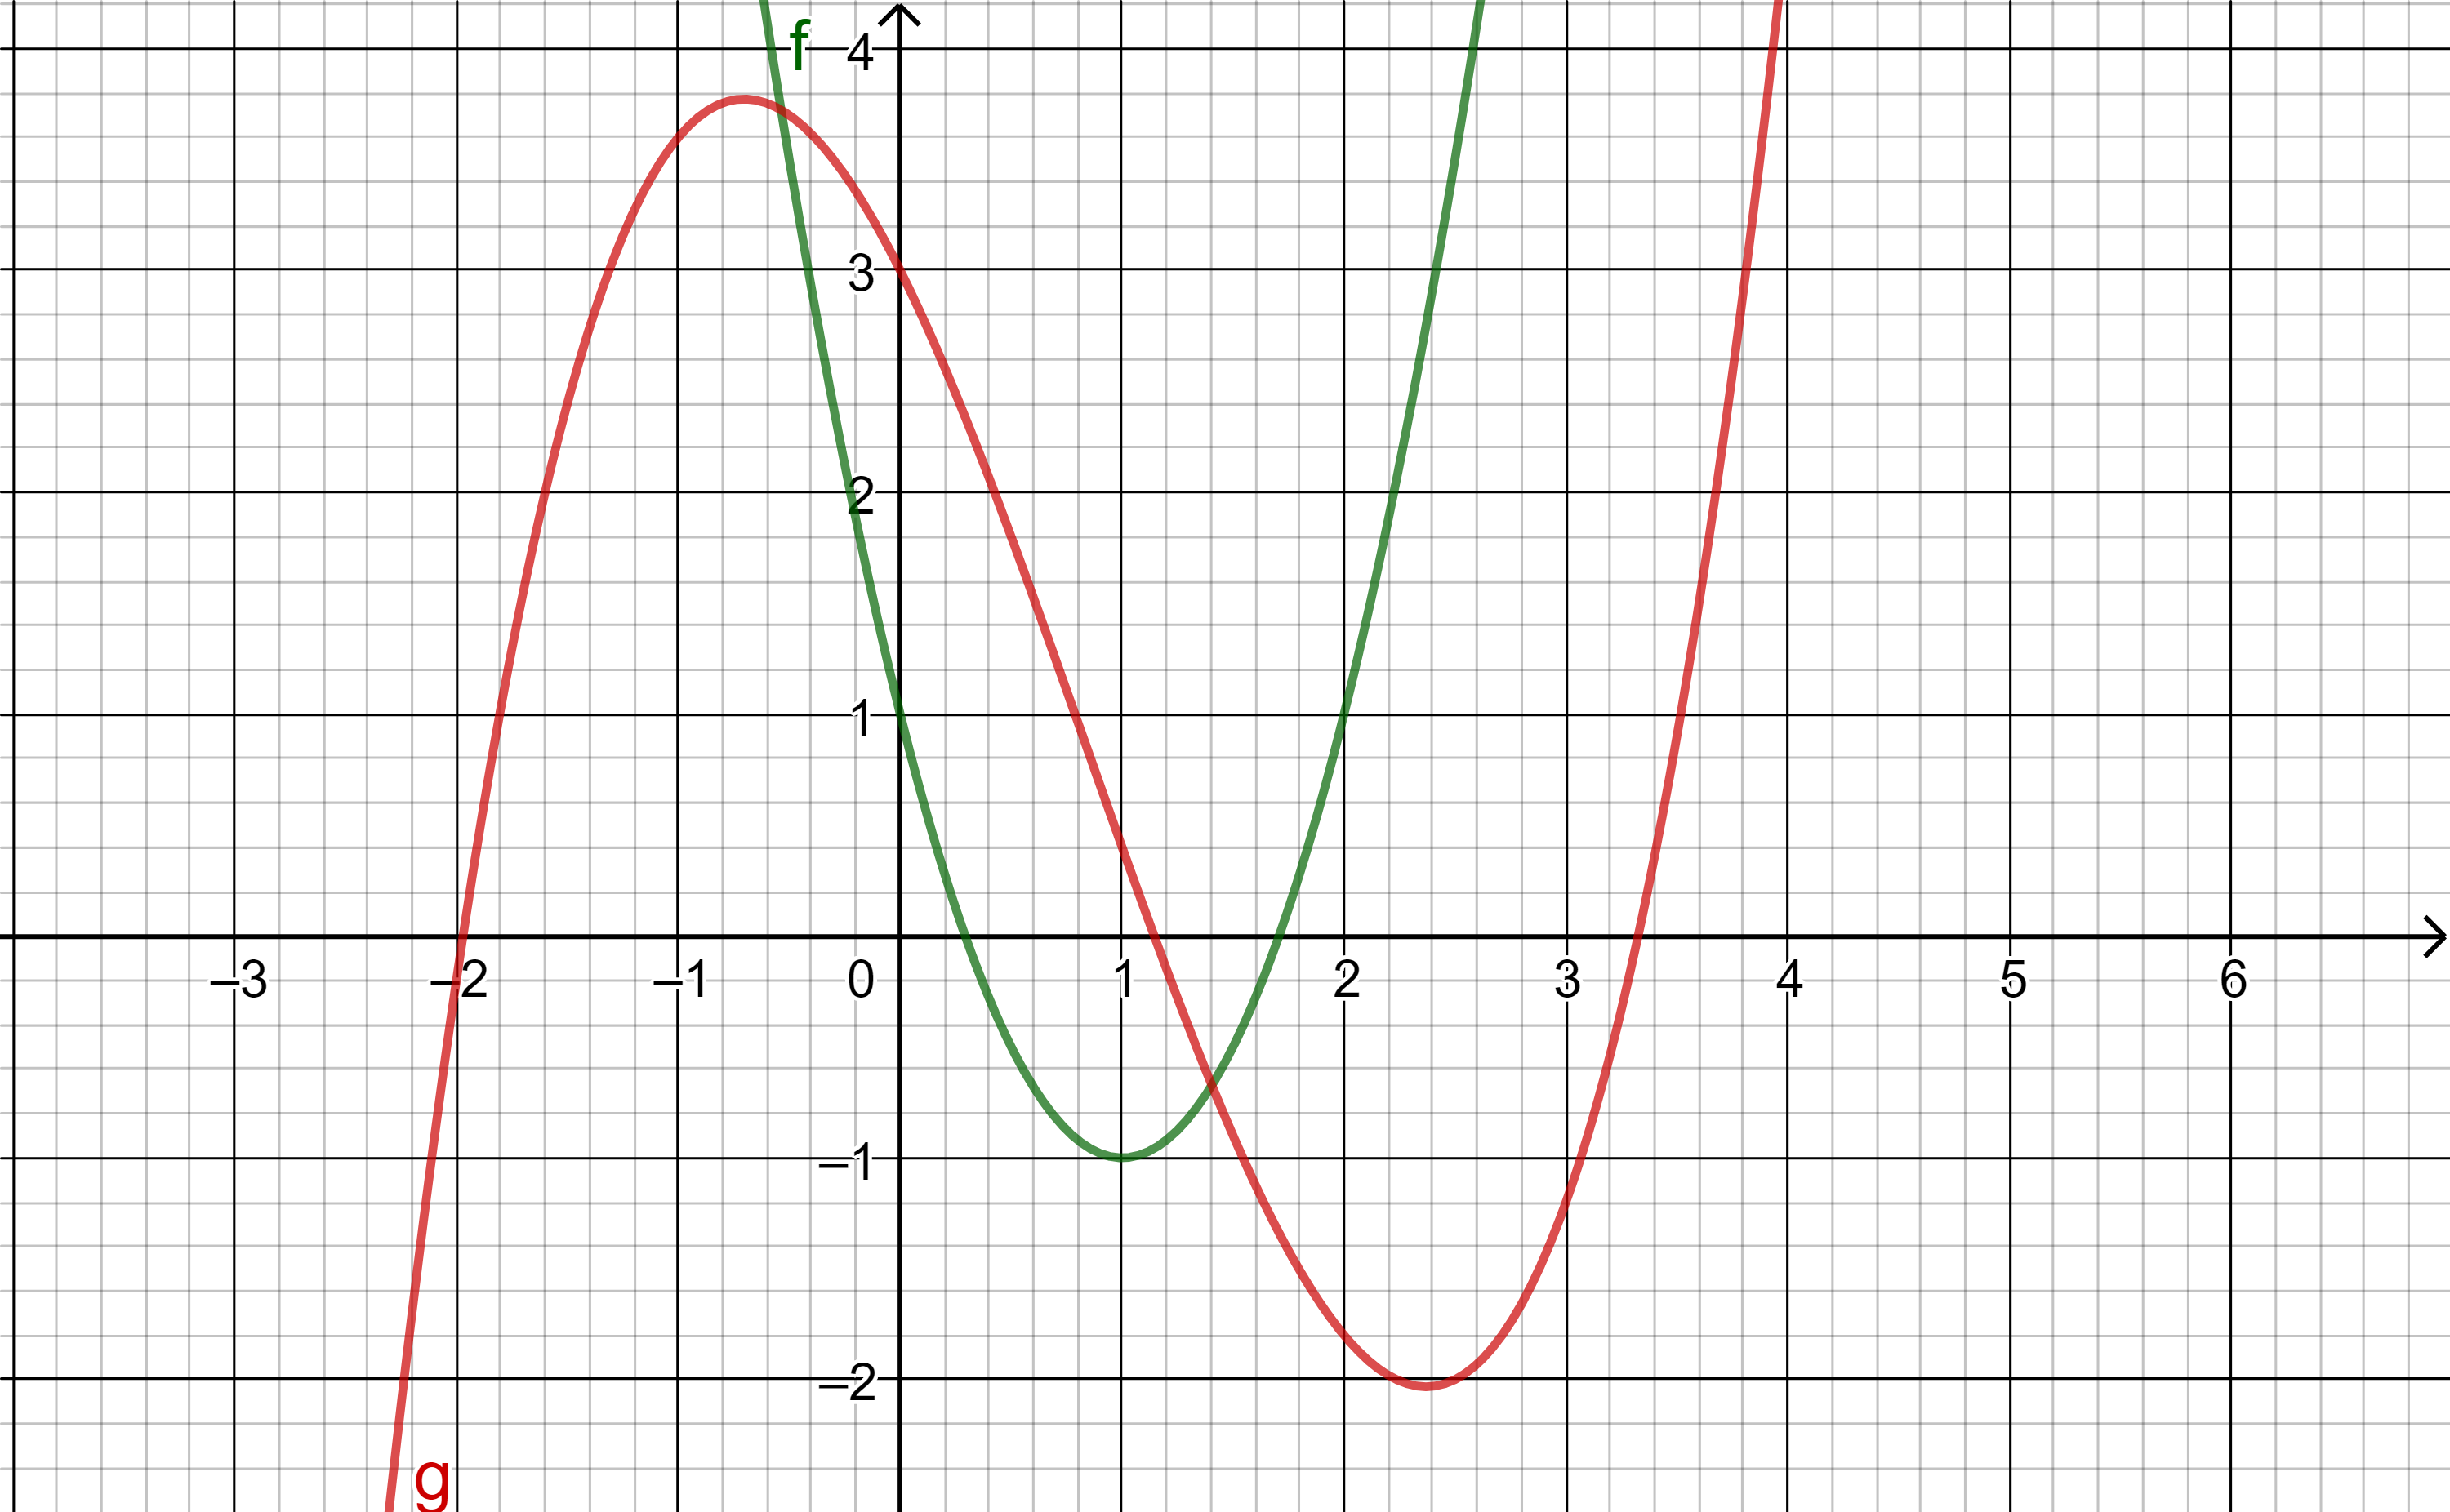
\includegraphics[width=0.5\textwidth]{pics/graphen}\\
         Bestimme die Stellen (ungefähr) bei denen der Funktionswert von f und der von g übereinstimmt.\\
    }
    \solution{$\frac{-1}{2}$ und $\frac{3}{2}$
    }
\end{Add}

\begin{Add}{MaI}{basal1.2}{Funktionen}{schwieriger}
    \question{
        Gegeben sind die Graphen der Funktionen f und g. \\
        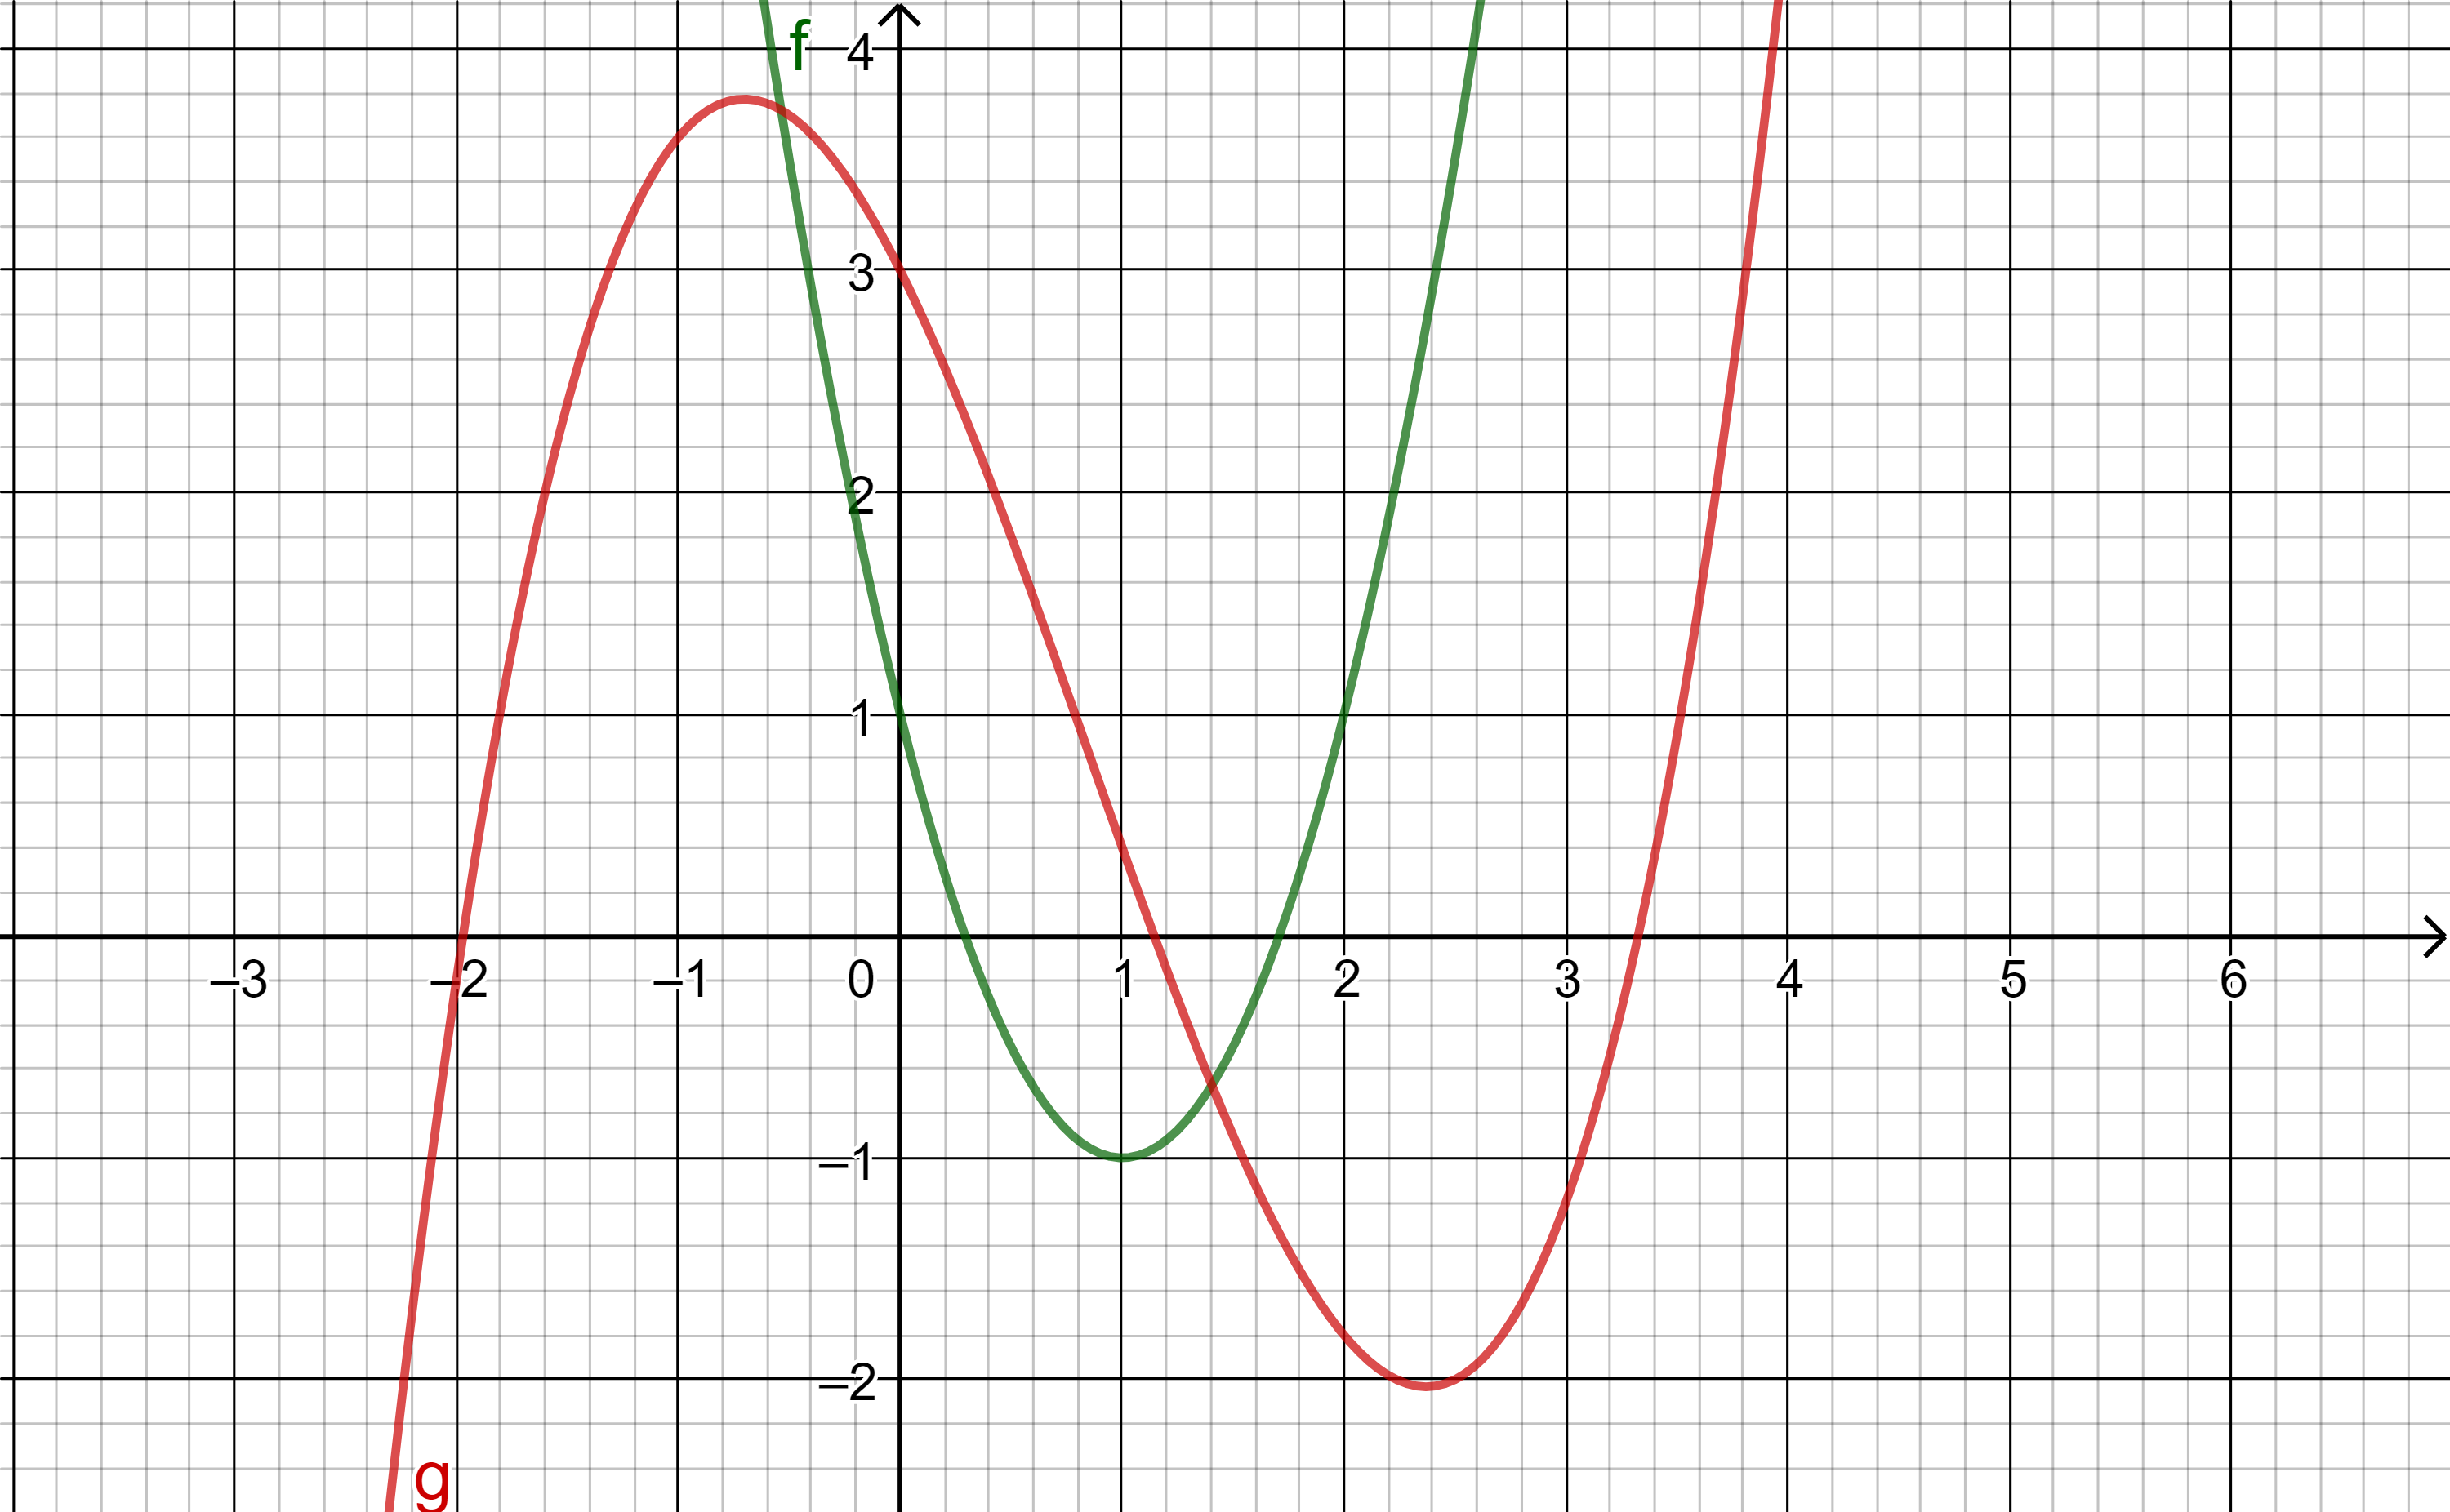
\includegraphics[width=0.5\textwidth]{pics/graphen}\\
        Bestimme den Funktionswert von f an der Stelle $x=0$.\\
    }
    \solution{
        $1$
    }
\end{Add}

\begin{Add}{MaI}{basal1.2}{Funktionen}{schwieriger}
    \question{
        Gegeben sind die Graphen der Funktionen f und g. \\
        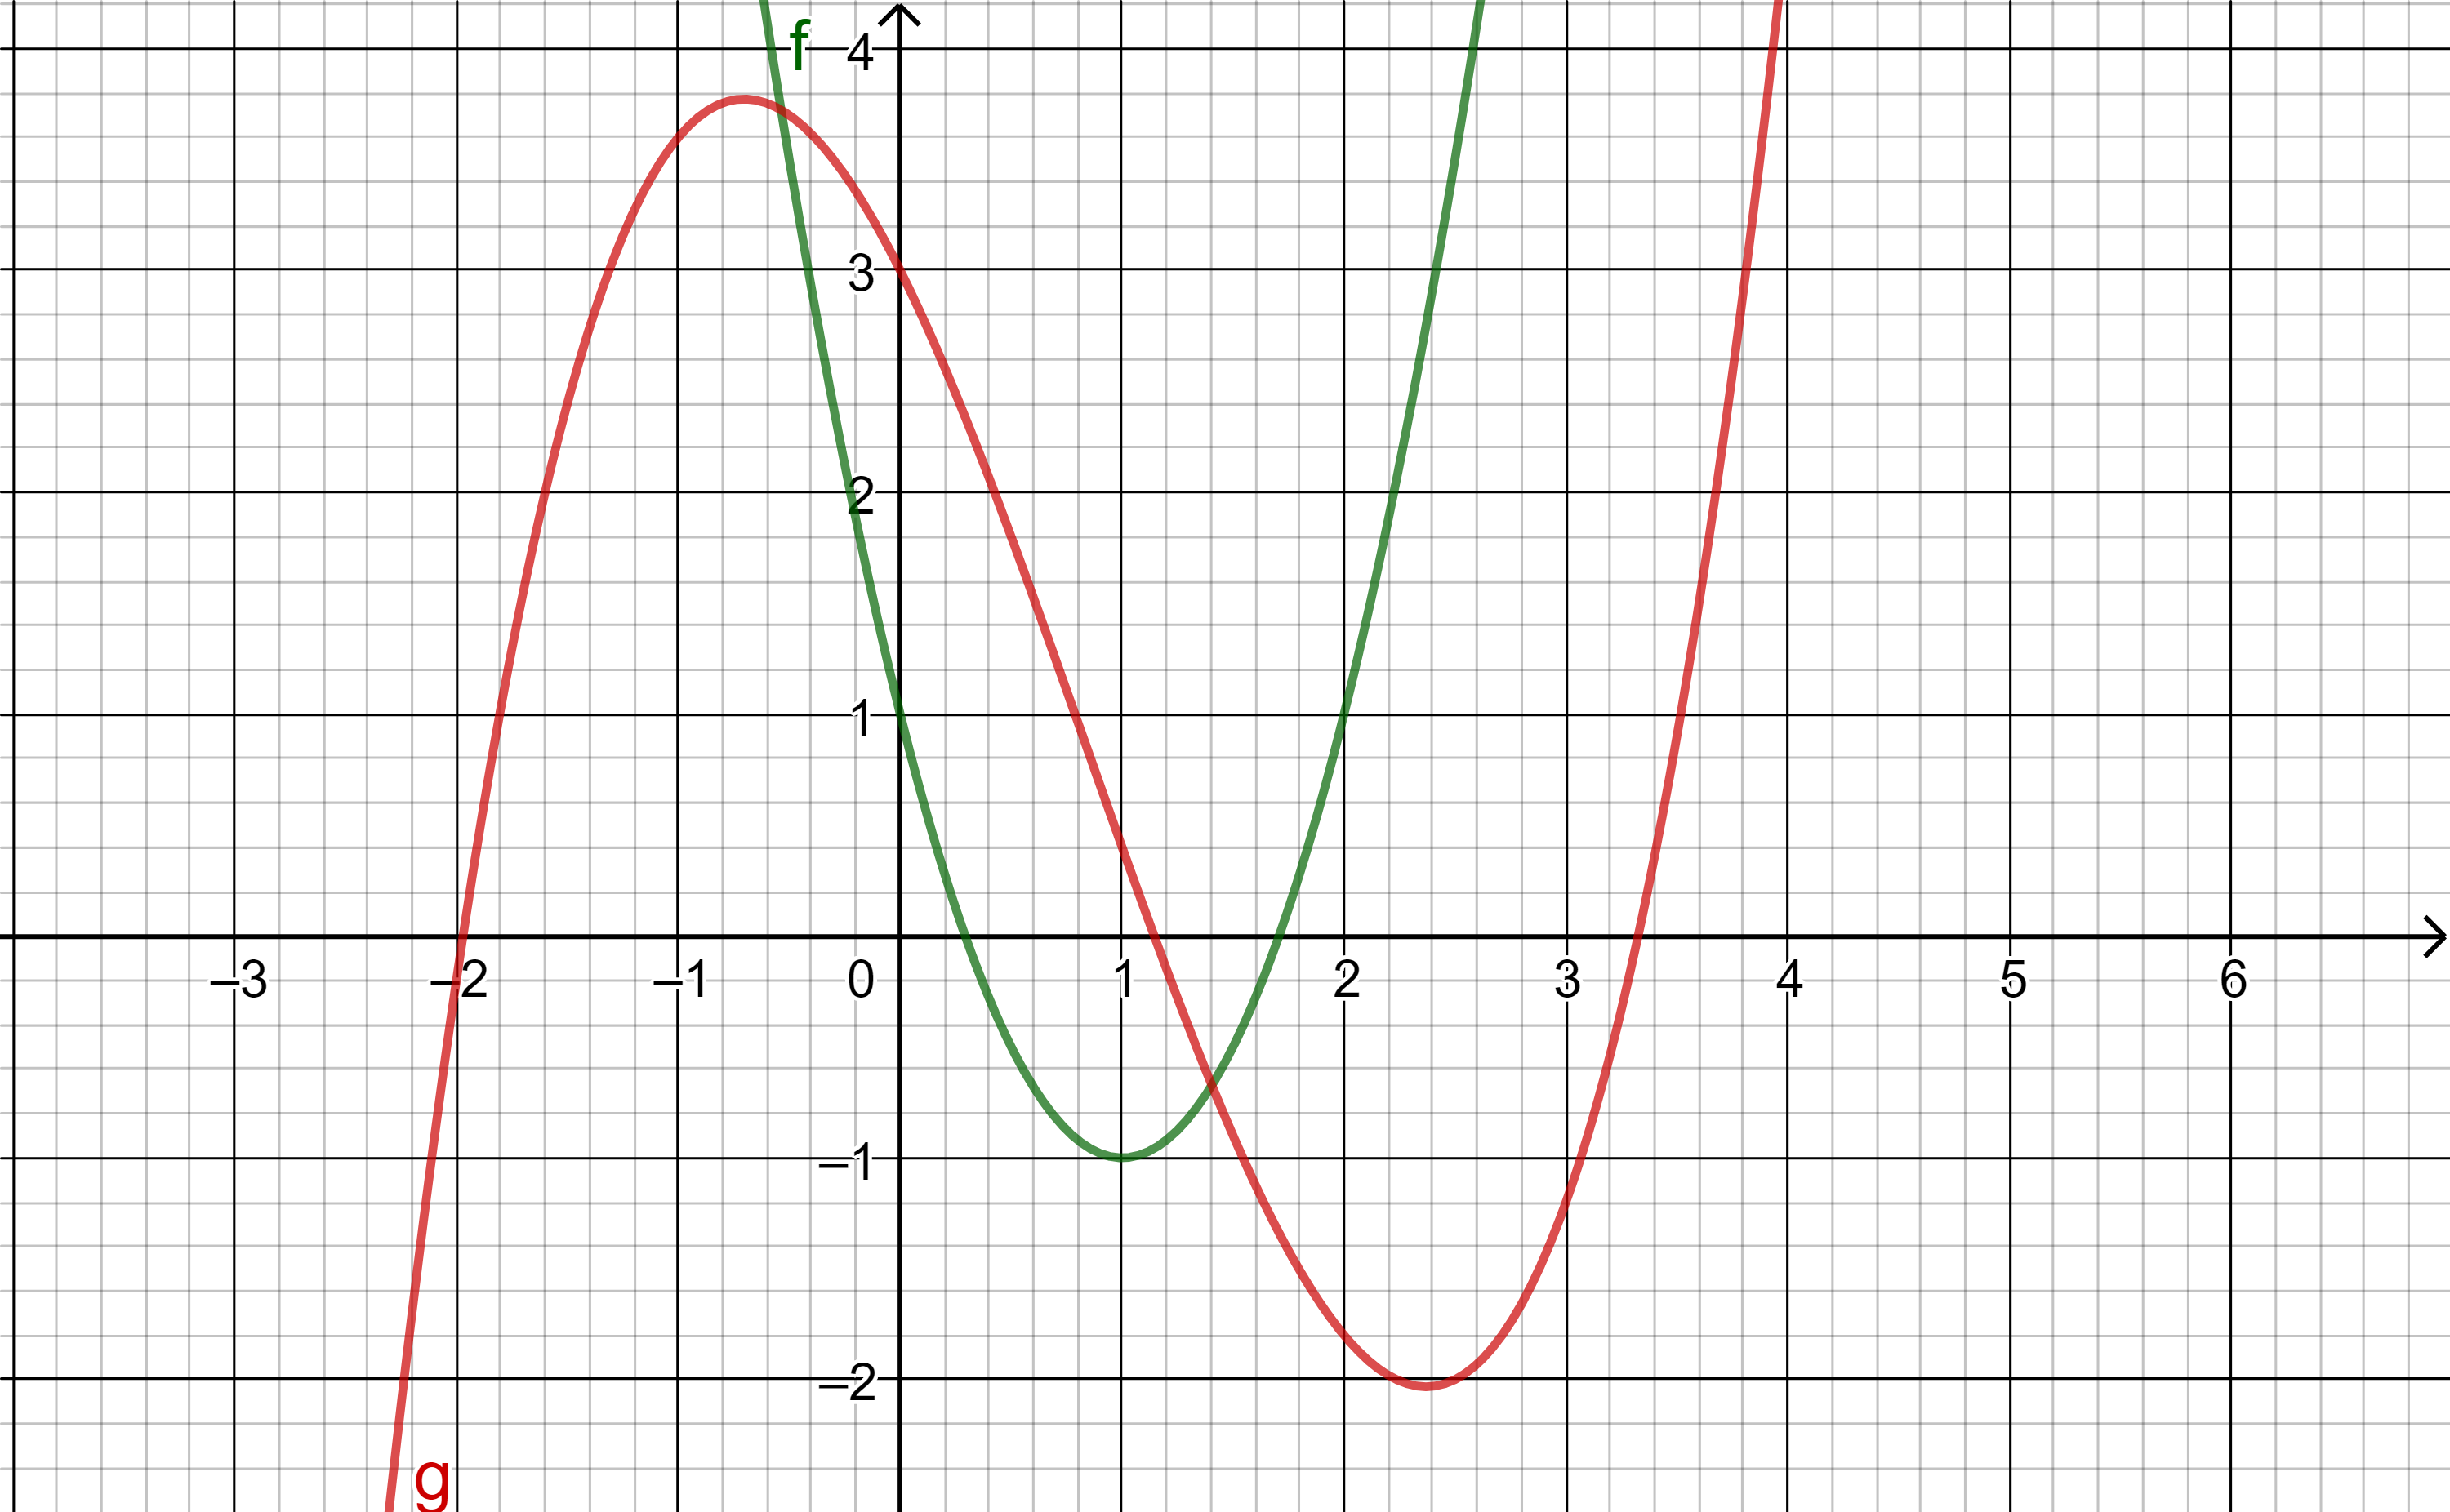
\includegraphics[width=0.5\textwidth]{pics/graphen}\\
        An welcher Stelle ist der Funktionswert von f gleich $-1$.\\
    }
    \solution{
        $1$
    }
\end{Add}

\begin{Add}{MaI}{basal1.2}{Funktionen}{schwieriger}
    \question{
        Gegeben sind die Graphen der Funktionen f und g. \\
        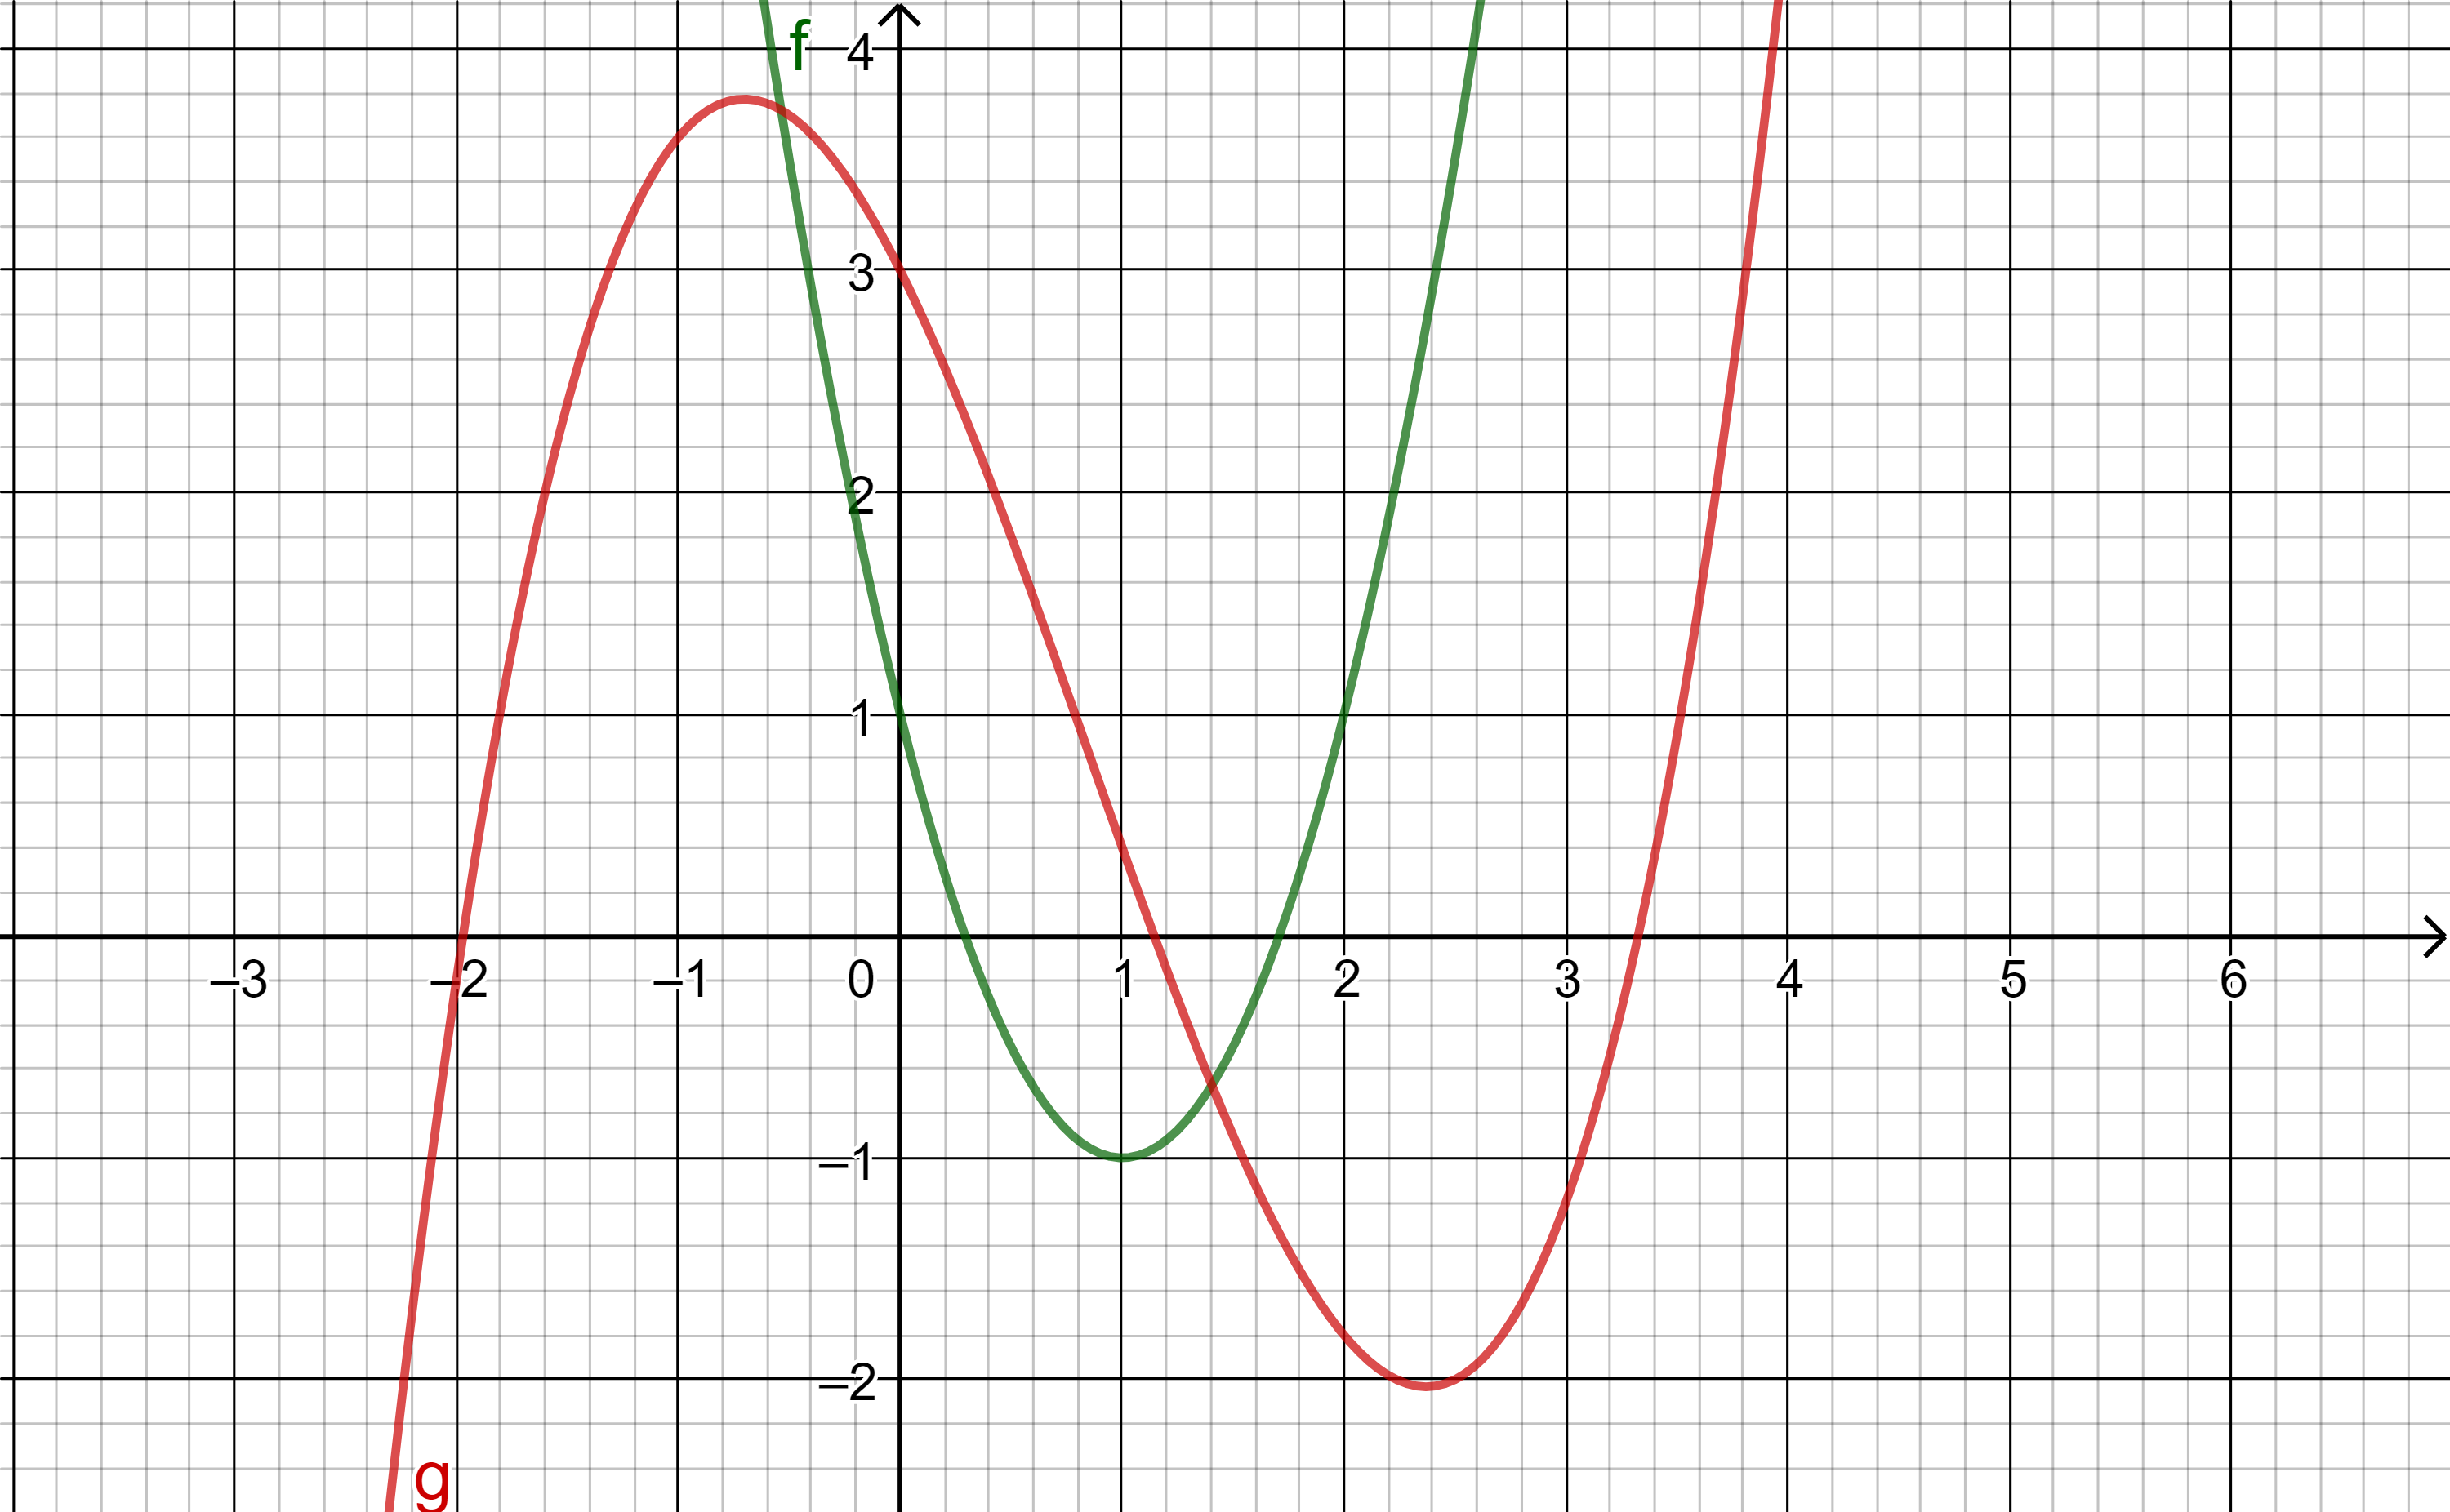
\includegraphics[width=0.5\textwidth]{pics/graphen}\\
        Bestimme den Funktionswert von g an der Stelle $x=0$.\\
    }
    \solution{
        $3$
    }
\end{Add}

\begin{Add}{MaI}{basal1.1}{Wurzelterme}{einfach}
    \question{
       Vereinfache:
        $$\sqrt{a^2+b^2}=\;?$$
        $$\sqrt{a^2 \cdot b^2}=\;?$$
        $$\sqrt{\frac{a^2}{b^2}}=\;?$$
    }
    \solution{
        $\sqrt{a^2+b^2}$ , $a \cdot b$ und $\frac{a}{b}$ 
    }
\end{Add}

\begin{Add}{MaI}{basal1.1}{Faktorisieren,Wurzelterme}{schwieriger}
    \question{
       Vereinfache:
        $$\sqrt{4a^2+4a+1}=\;?$$
    }
    \solution{
        $2a+1$ 
    }
\end{Add}

\begin{Add}{MaI}{basal1.1}{Faktorisieren,Wurzelterme}{schwieriger}
    \question{
       Vereinfache:
        $$\sqrt{36x^2+24x+4}=\;?$$
    }
    \solution{
        $2(3x+1)$ 
    }
\end{Add}

\begin{Add}{MaI}{basal1.1}{Faktorisieren,Wurzelterme}{schwieriger}
    \question{
       Vereinfache:
        $$\sqrt{4a^2x^2-36a^2}=\;?$$
    }
    \solution{
        $2a\sqrt{(x+3)(x-3)}$ 
    }
\end{Add}
\begin{Add}{MaI}{basal1.1}{Faktorisieren,Wurzelterme}{schwieriger}
    \question{
       Vereinfache:
        $$\sqrt{a^4-4a^3b+4a^2b^2}=\;?$$

    }
    \solution{
        $a(a-2b)$ 
    }
\end{Add}

\begin{Add}{MaI}{basal1.1}{Faktorisieren}{schwieriger}
    \question{
       Faktorisiere:
        $$x^4y^2-x^2y^4$$
    }
    \solution{
        $x^2y^2(x-y)(x+y)$
    }
\end{Add}

\begin{Add}{MaI}{basal1.1}{Faktorisieren}{schwieriger}
    \question{
       Faktorisiere:
        $$3x^2y^2-3x^2z^2$$
    }
    \solution{
        $3x^2(y-z)(y+z)$
    }
\end{Add}

\begin{Add}{MaI}{basal1.1}{Bruchterme}{schwieriger}
    \question{
       Fasse zusammen:
        $$\frac{3z}{x^2y}+\frac{z^2}{xy^3}+\frac{2z^3}{x^3y^2}$$
    }
    \solution{
        $\frac{3xy^2z+x^2z^2+2yz^3}{x^3y^3}$
    }
\end{Add}

\begin{Add}{MaI}{basal1.1}{Bruchterme}{schwieriger}
    \question{
       Vereinfache:
        $$\frac{p^7}{r}\left(\frac{q^5}{p^4}\div\frac{q^8}{r^4}\right)$$
    }
    \solution{
        $\frac{p^3r^3}{q^3}$
    }
\end{Add}

\begin{Add}{MaI}{basal1.1}{Faktorisieren,Bruchterme}{schwieriger}
    \question{
       Fasse zusammen:
         $$\frac{2a}{3a-3b}+\frac{a-b}{a-b}+\frac{b}{3a}$$
    }
    \solution{
         $\frac{5a^2-2ab-b^2}{3a(a-b)}$
    }
\end{Add}

\begin{Add}{MaI}{basal1.1}{Faktorisieren,Bruchterme}{schwieriger}
    \question{
       Fasse zusammen:
         $$2+\frac{3z^2}{z^2-yz}-\frac{y}{z-y}$$
    }
    \solution{
         $\frac{5z-3y}{z-y}$
    }
\end{Add}

\begin{Add}{MaI}{basal1.1}{Bruchterme}{schwieriger}
    \question{
       Berechne:
         $$\frac{a^2}{bc}\div\left(1-\frac{a}{c}\right)$$
    }
    \solution{
         $\frac{a^2}{b(c-a)}$
    }
\end{Add}

\begin{Add}{MaI}{basal1.1}{Bruchterme}{schwieriger}
    \question{
       Berechne:
         $$\left(1-\frac{b}{a}\right)\cdot\frac{ab}{a-b}$$
    }
    \solution{
         $b$
    }
\end{Add}

\begin{Add}{MaI}{basal1.1}{Bruchterme}{schwieriger}
    \question{
       Berechne:
         $$\frac{5}{xy}\div\left(\frac{1}{y}-\frac{1}{x}\right)$$
    }
    \solution{
         $\frac{5}{x-y}$
    }
\end{Add}

\begin{Add}{MaI}{basal1.1}{Bruchterme}{schwieriger}
    \question{
       Berechne:
         $$\left(1+\frac{b-a}{a}\right)\cdot\left(1-\frac{b}{b-a}\right)$$
    }
    \solution{
         $\frac{b}{a-b}$
    }
\end{Add}

\begin{Add}{MaI}{basal1.2}{Lineares,Funktionen}{schwieriger}
    \question{
        Gegeben ist der Graph der Funktion f. \\
        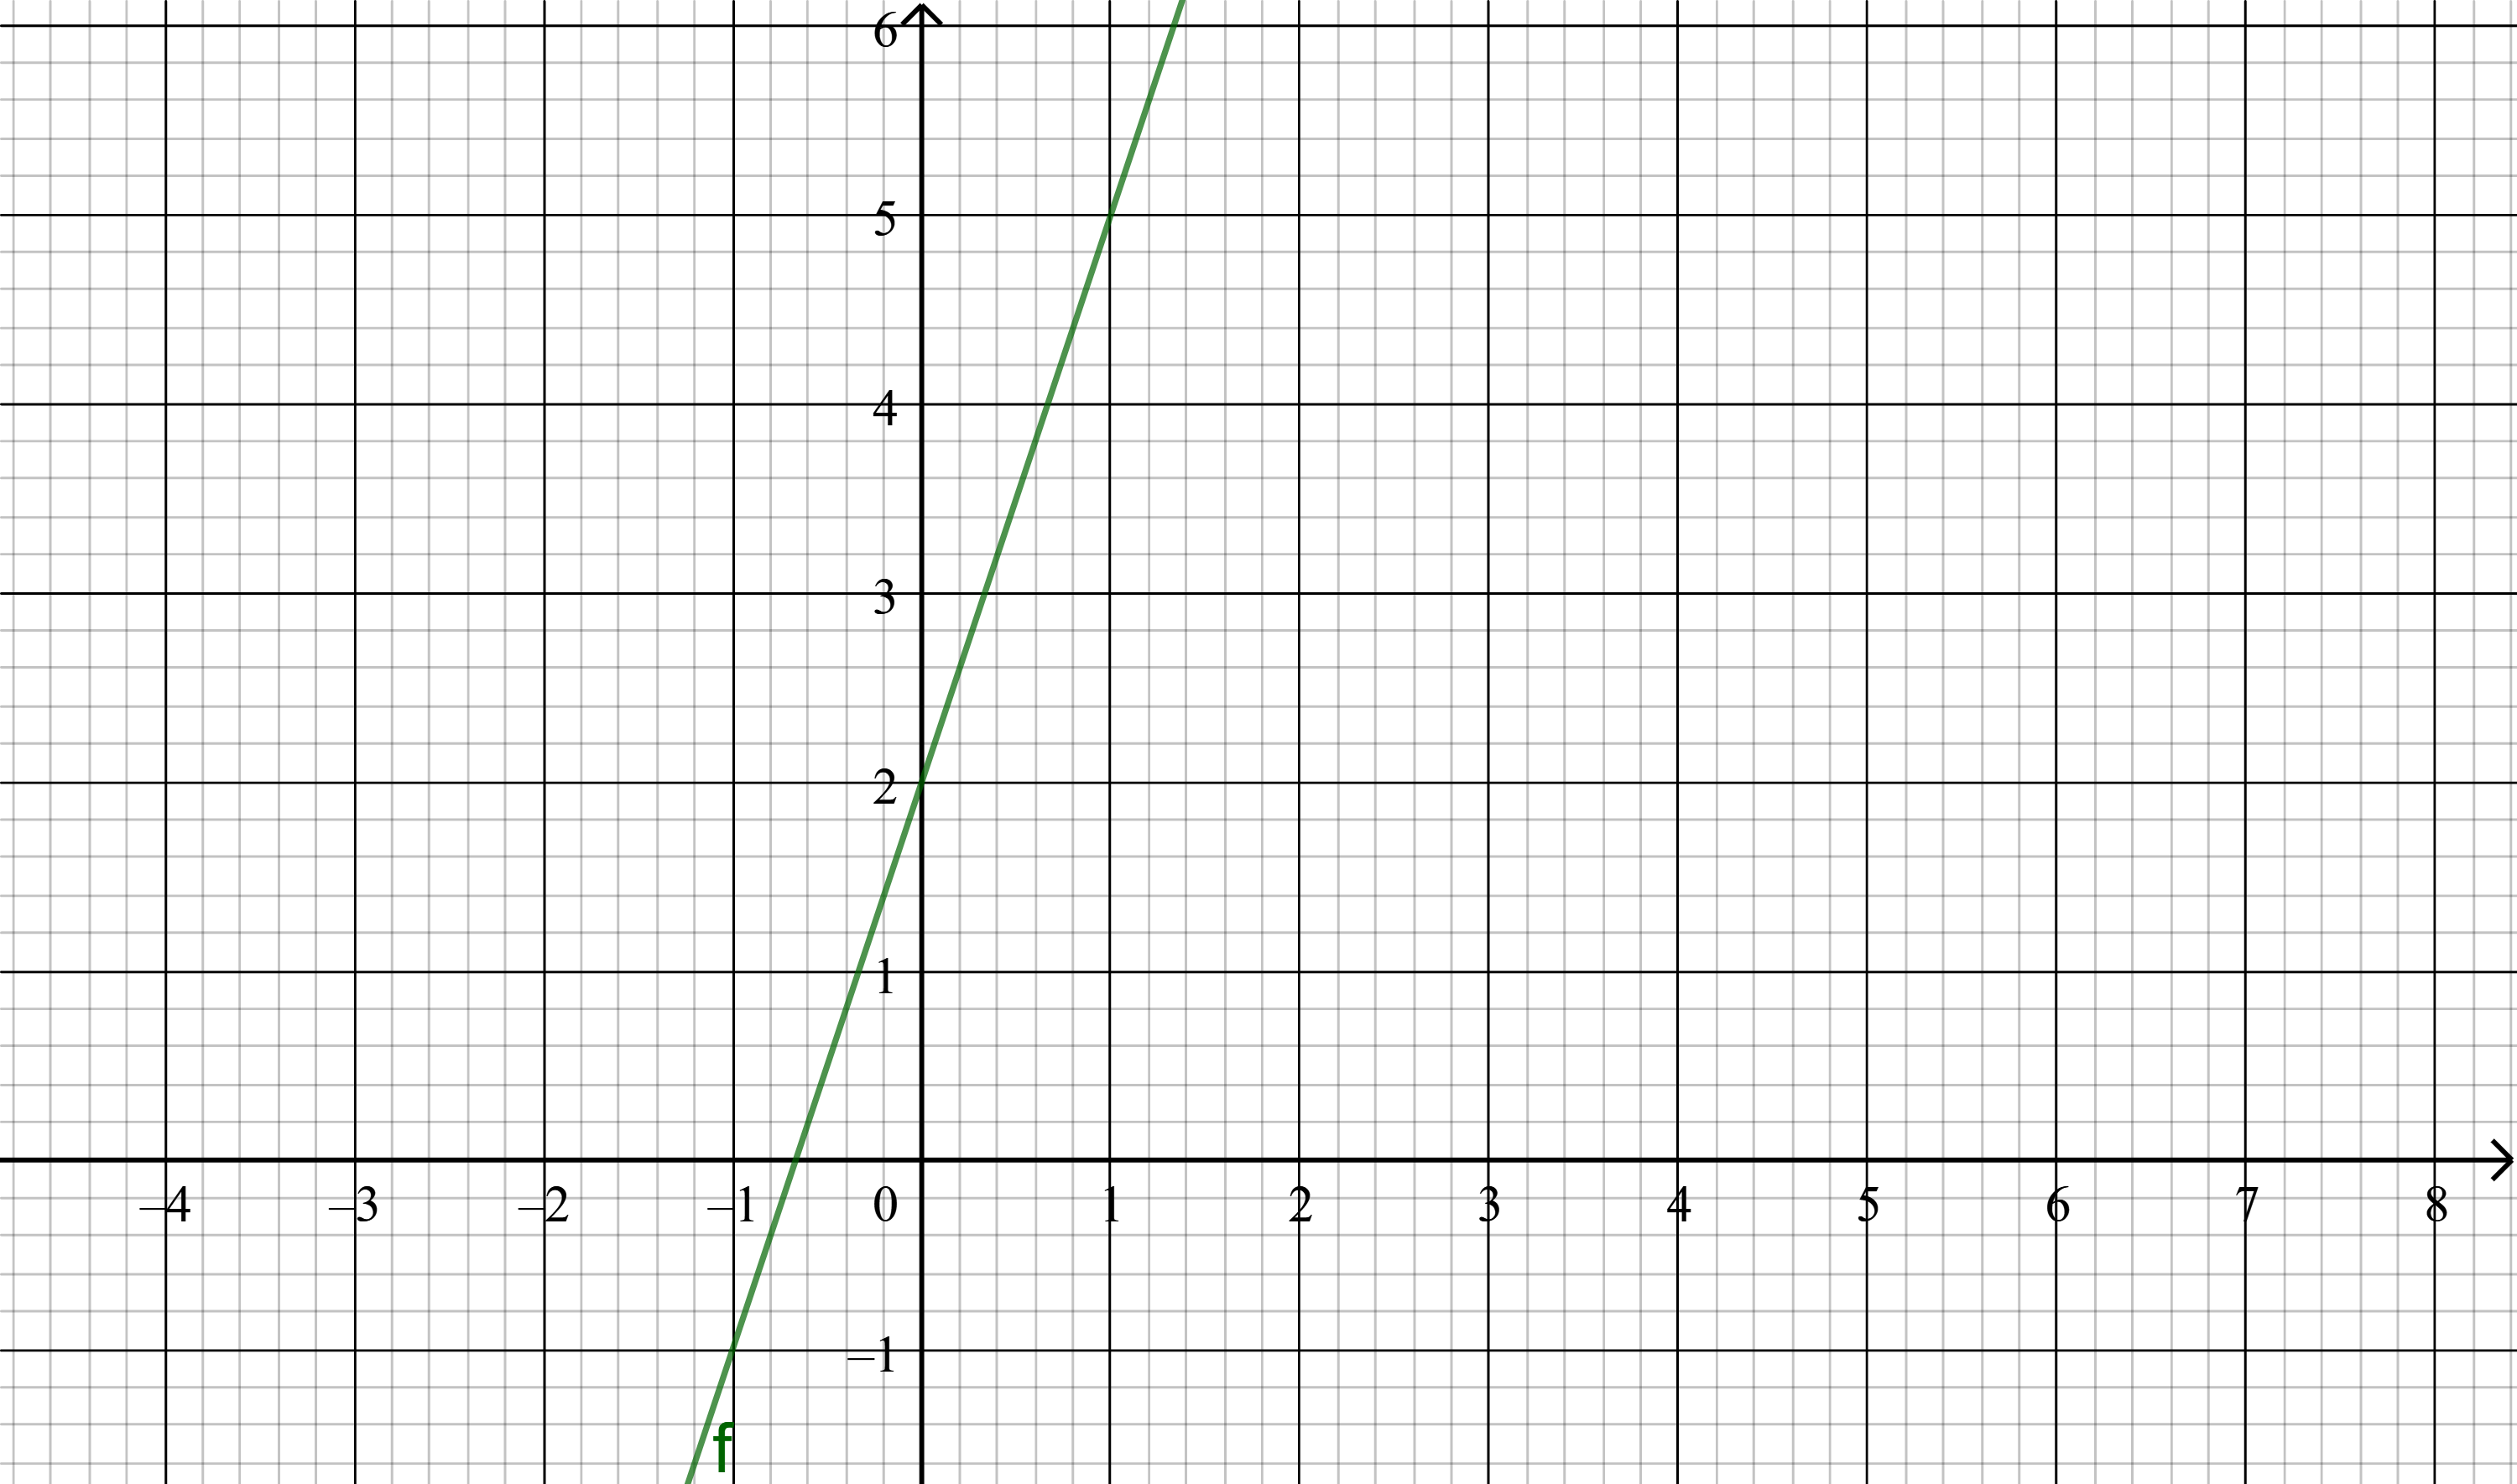
\includegraphics[width=0.5\textwidth]{pics/LinFunktion1}\\
         Bestimme die Funktionsgleichung von f.
    }
    \solution{$f(x)=3x+2$
    }
\end{Add}

\begin{Add}{MaI}{basal1.2}{Lineares,Funktionen}{schwieriger}
    \question{
        Gegeben ist der Graph der Funktion f. \\
        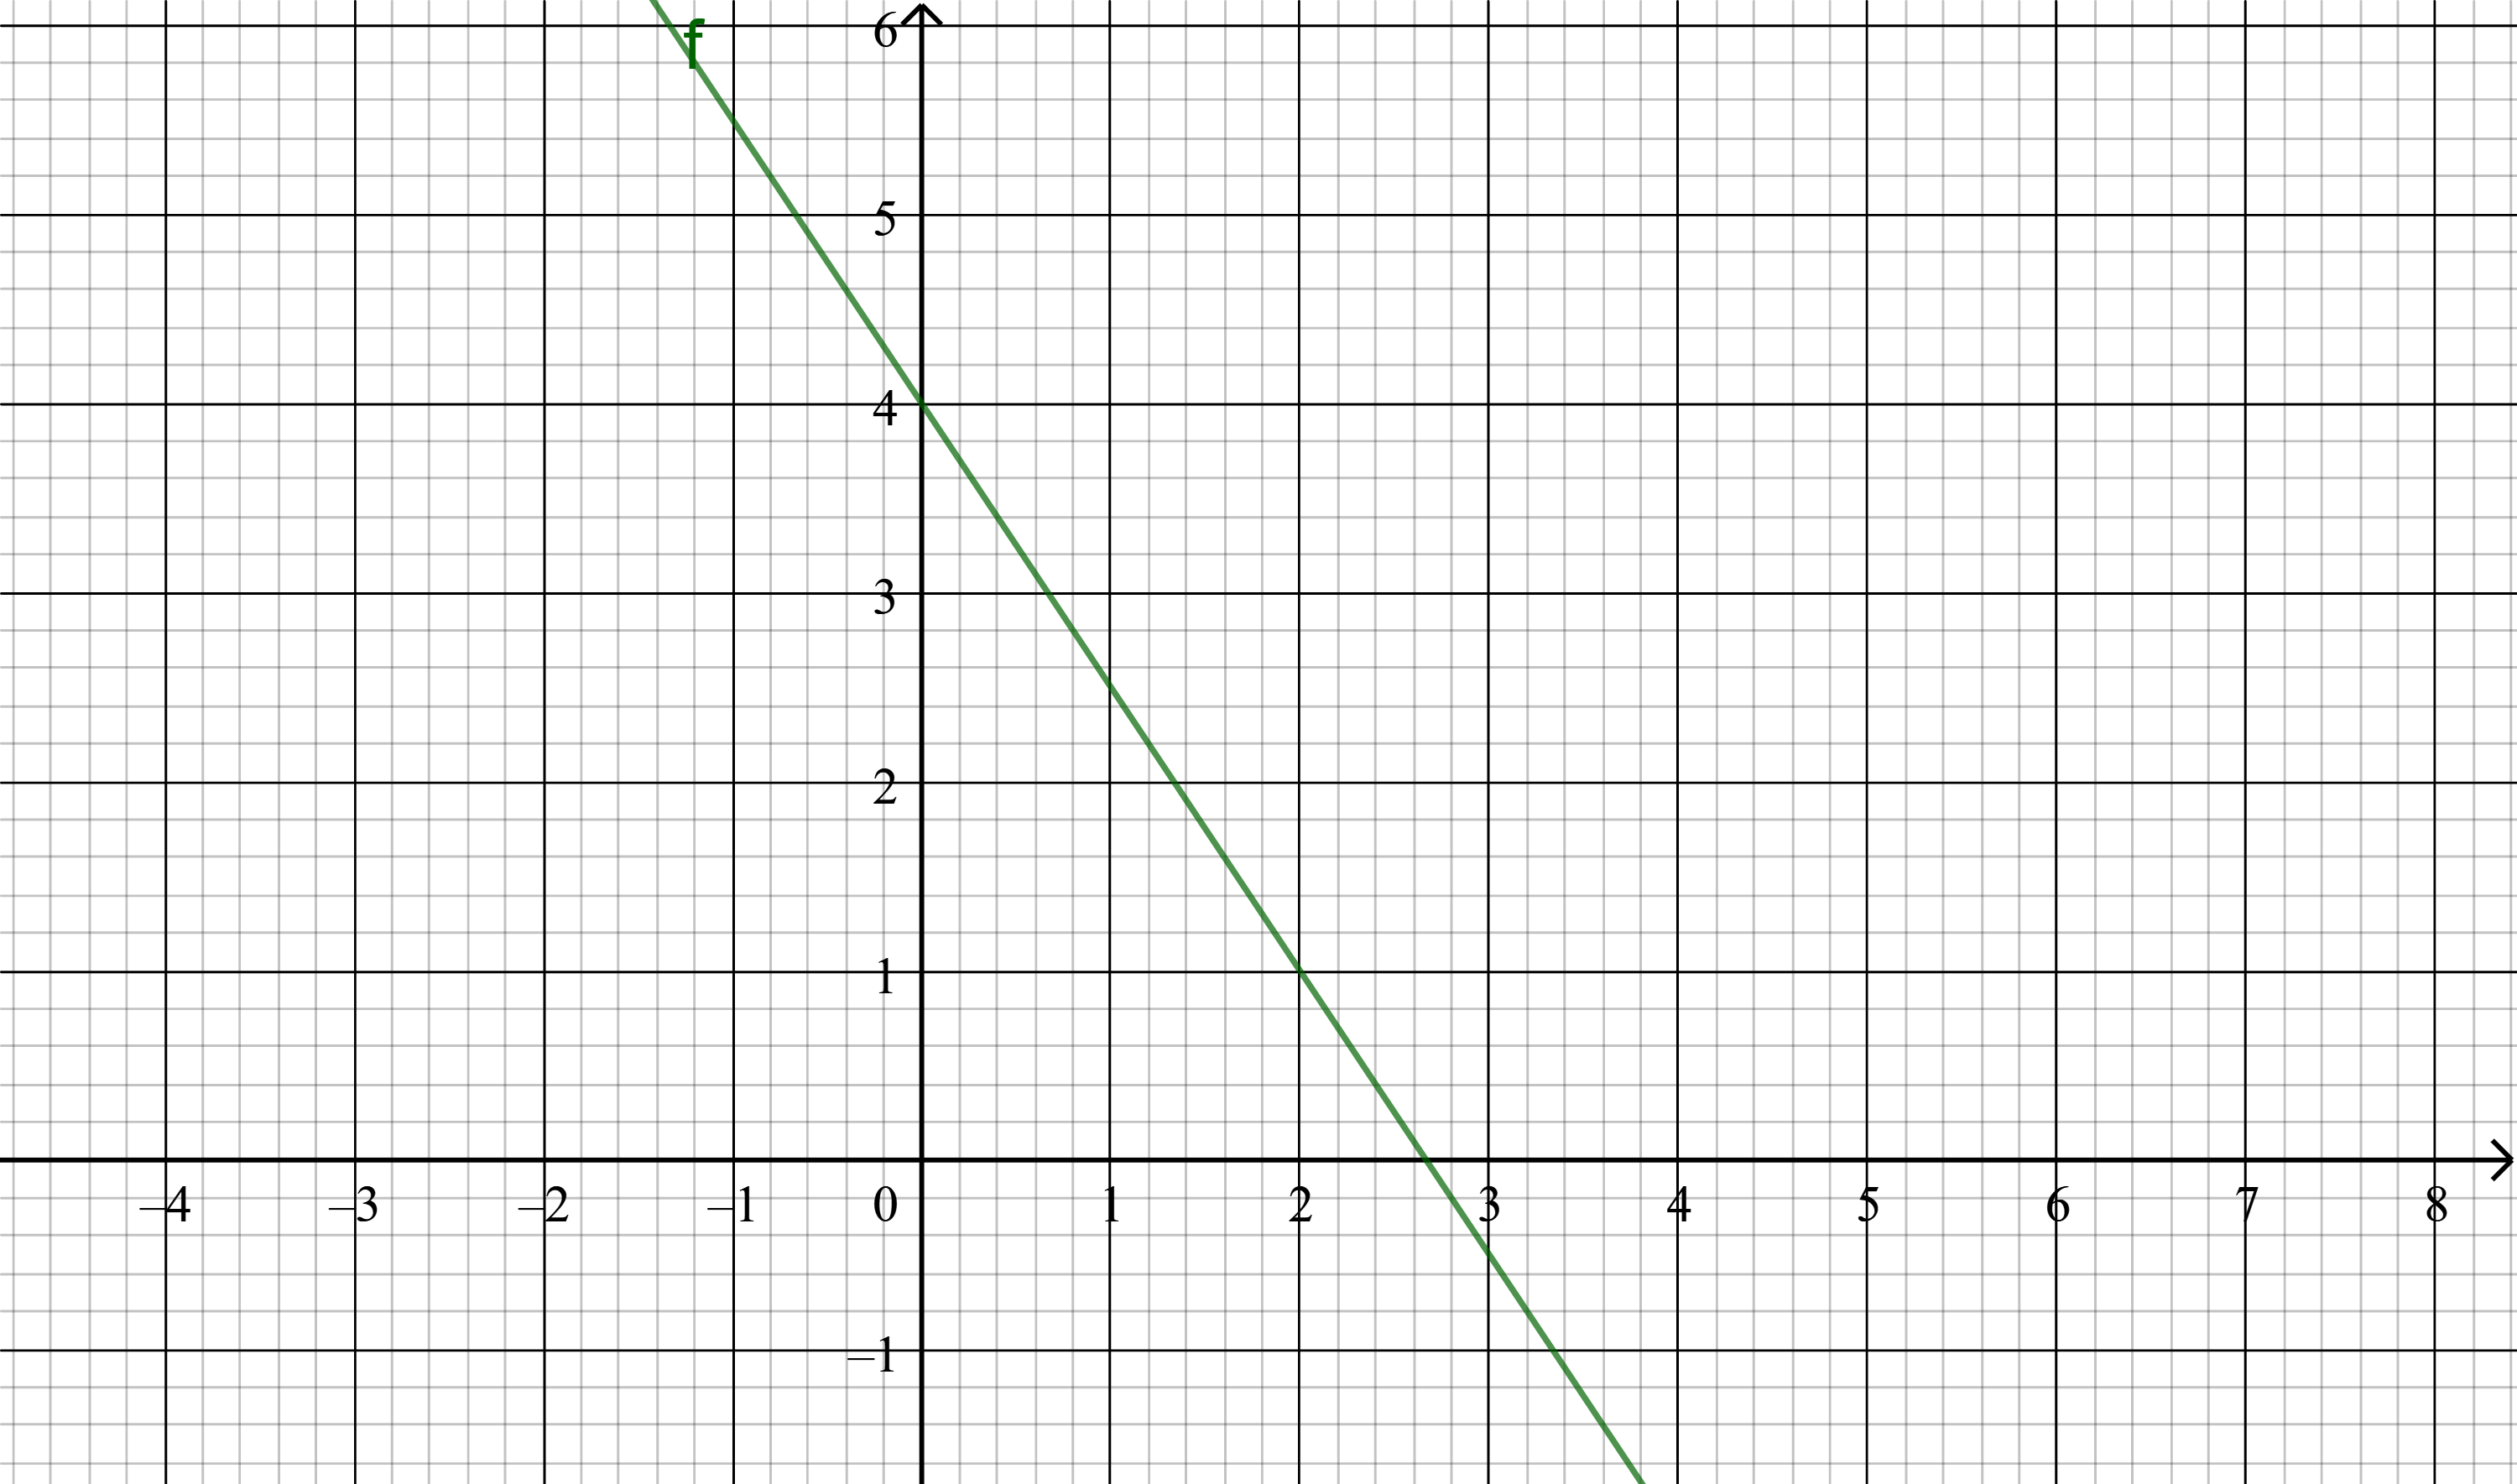
\includegraphics[width=0.5\textwidth]{pics/LinFunktion2}\\
         Bestimme die Funktionsgleichung von f.
    }
    \solution{$f(x)=-\frac{3}{2}x+4$
    }
\end{Add}

\begin{Add}{MaI}{basal1.2}{Lineares,Funktionen}{schwieriger}
    \question{
        Gegeben ist der Graph der Funktion f. \\
        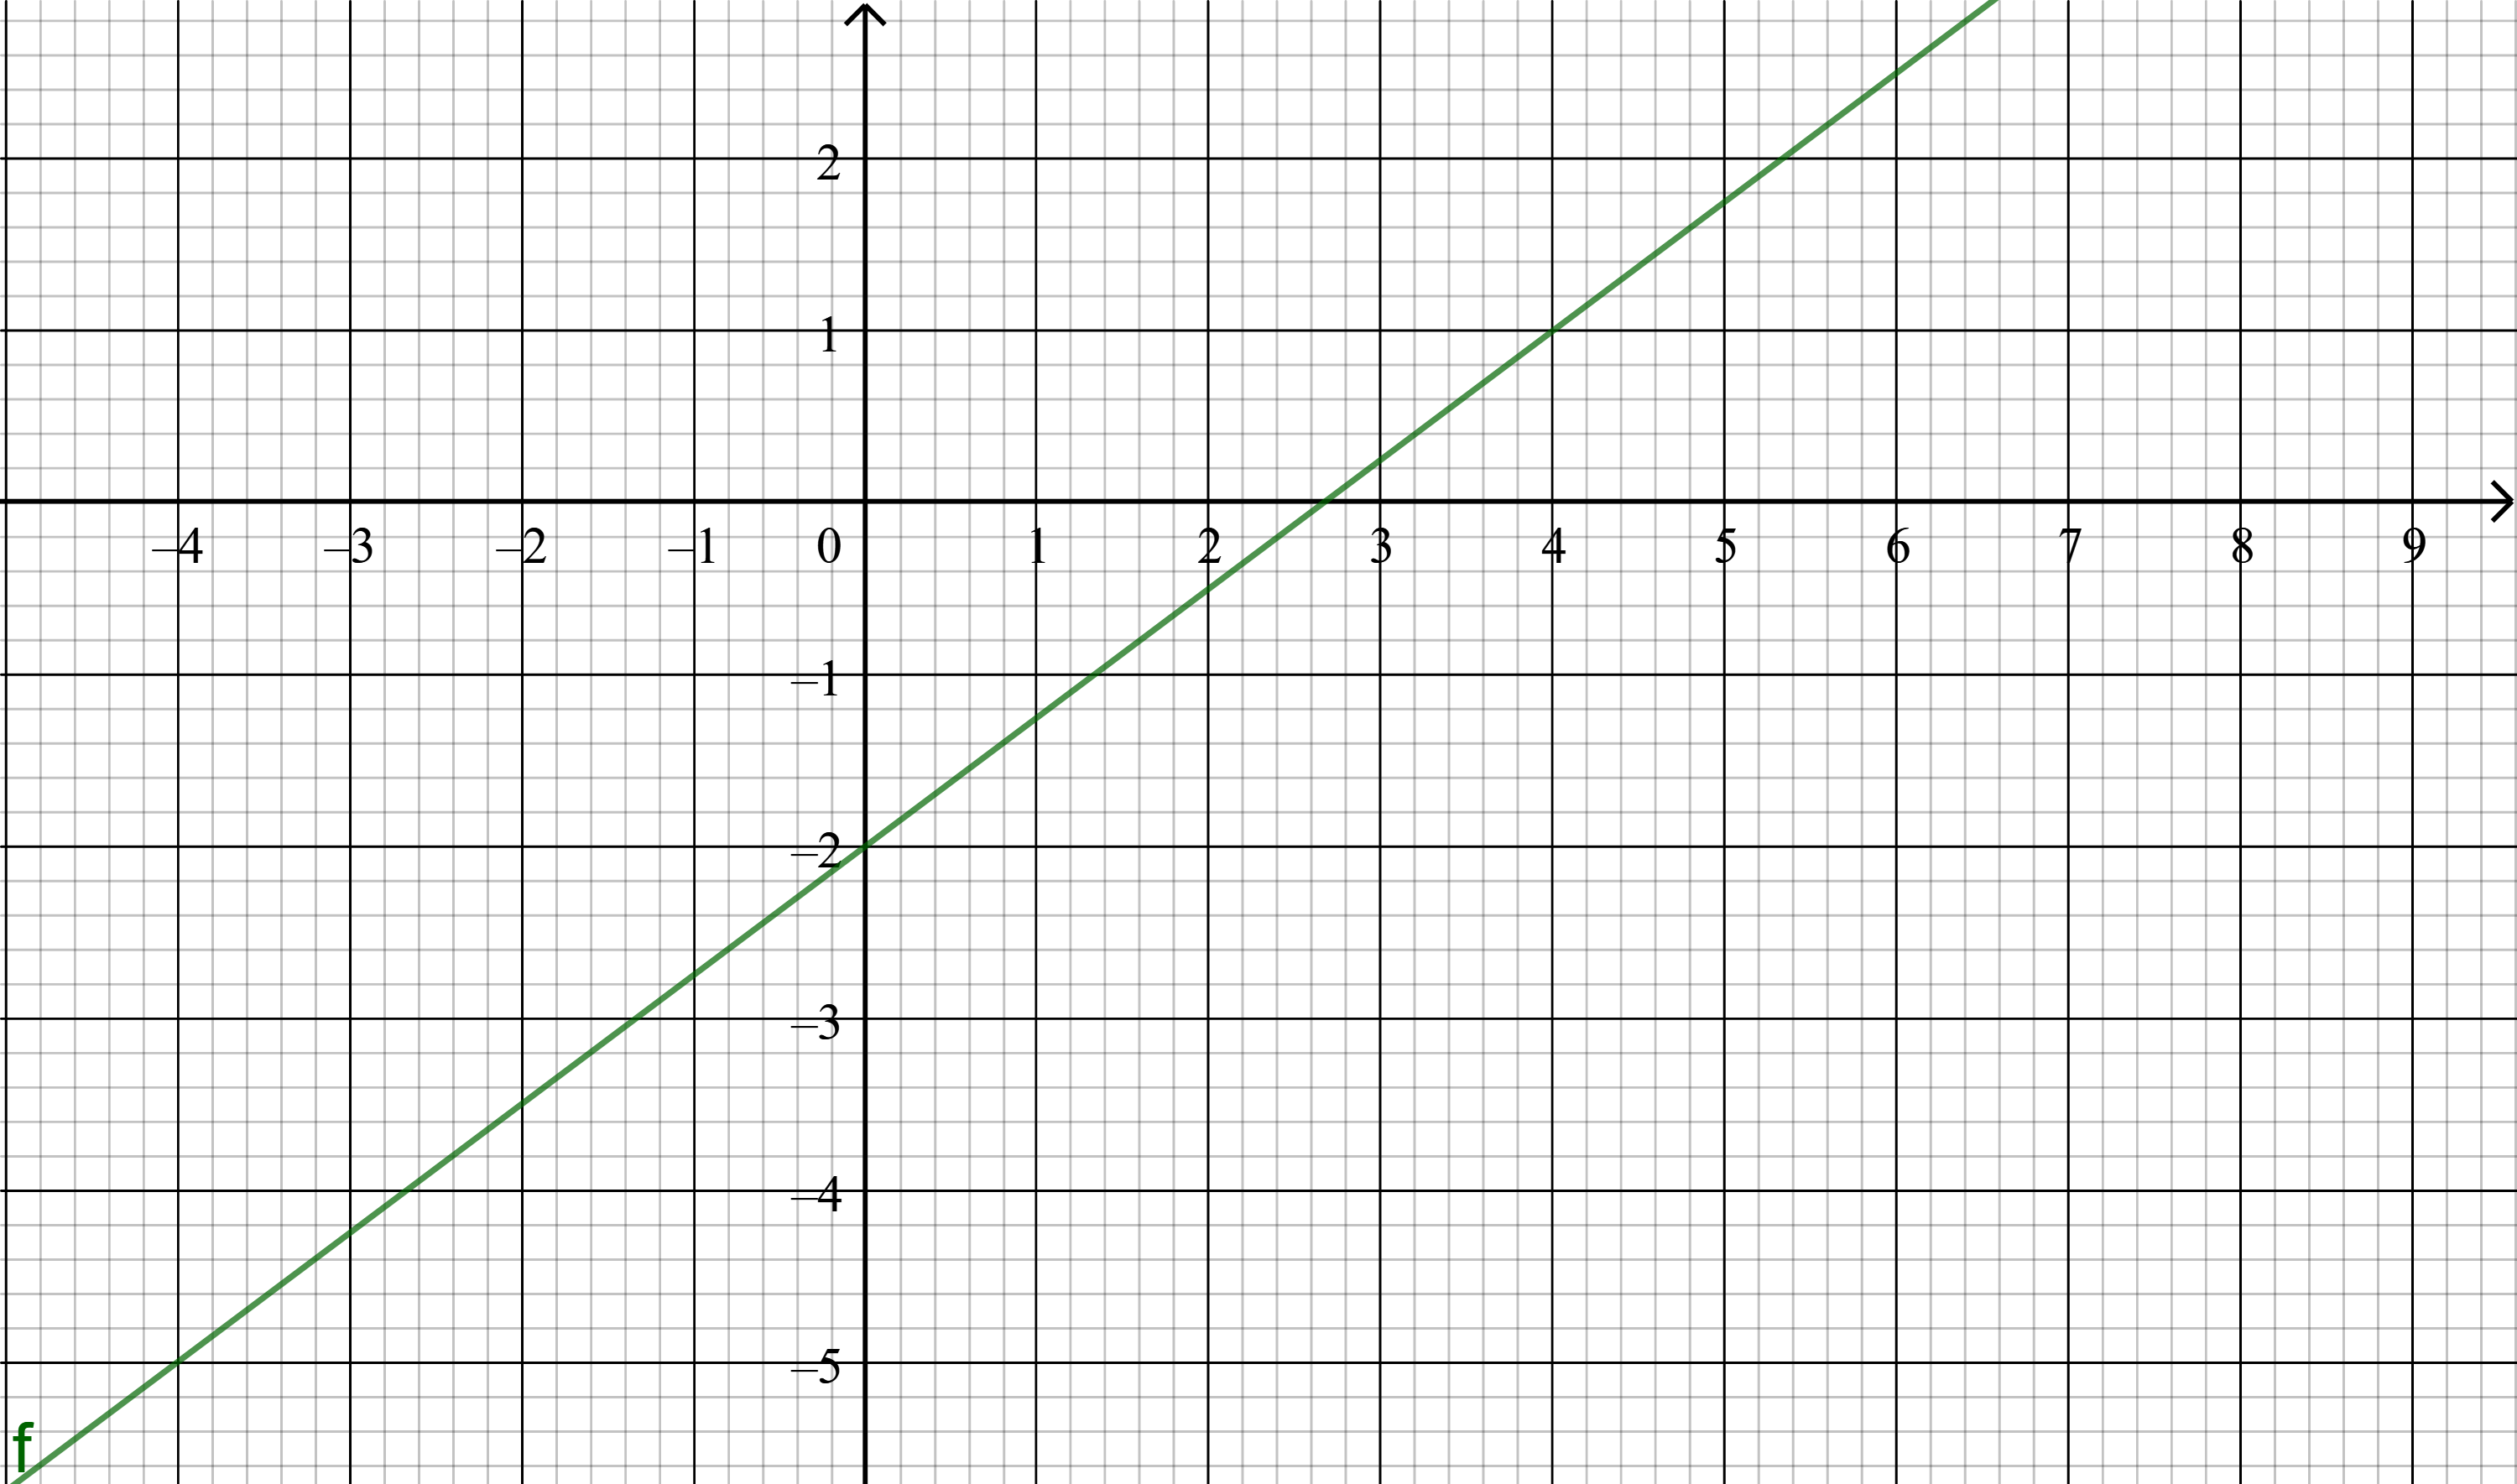
\includegraphics[width=0.5\textwidth]{pics/LinFunktion3}\\
         Bestimme die Funktionsgleichung von f.
    }
    \solution{$f(x)=\frac{3}{4}x-2$
    }
\end{Add}

\begin{Add}{MaI}{basal1.2}{Lineares,Funktionen}{schwieriger}
    \question{
        Gegeben ist der Graph der Funktion f. \\
        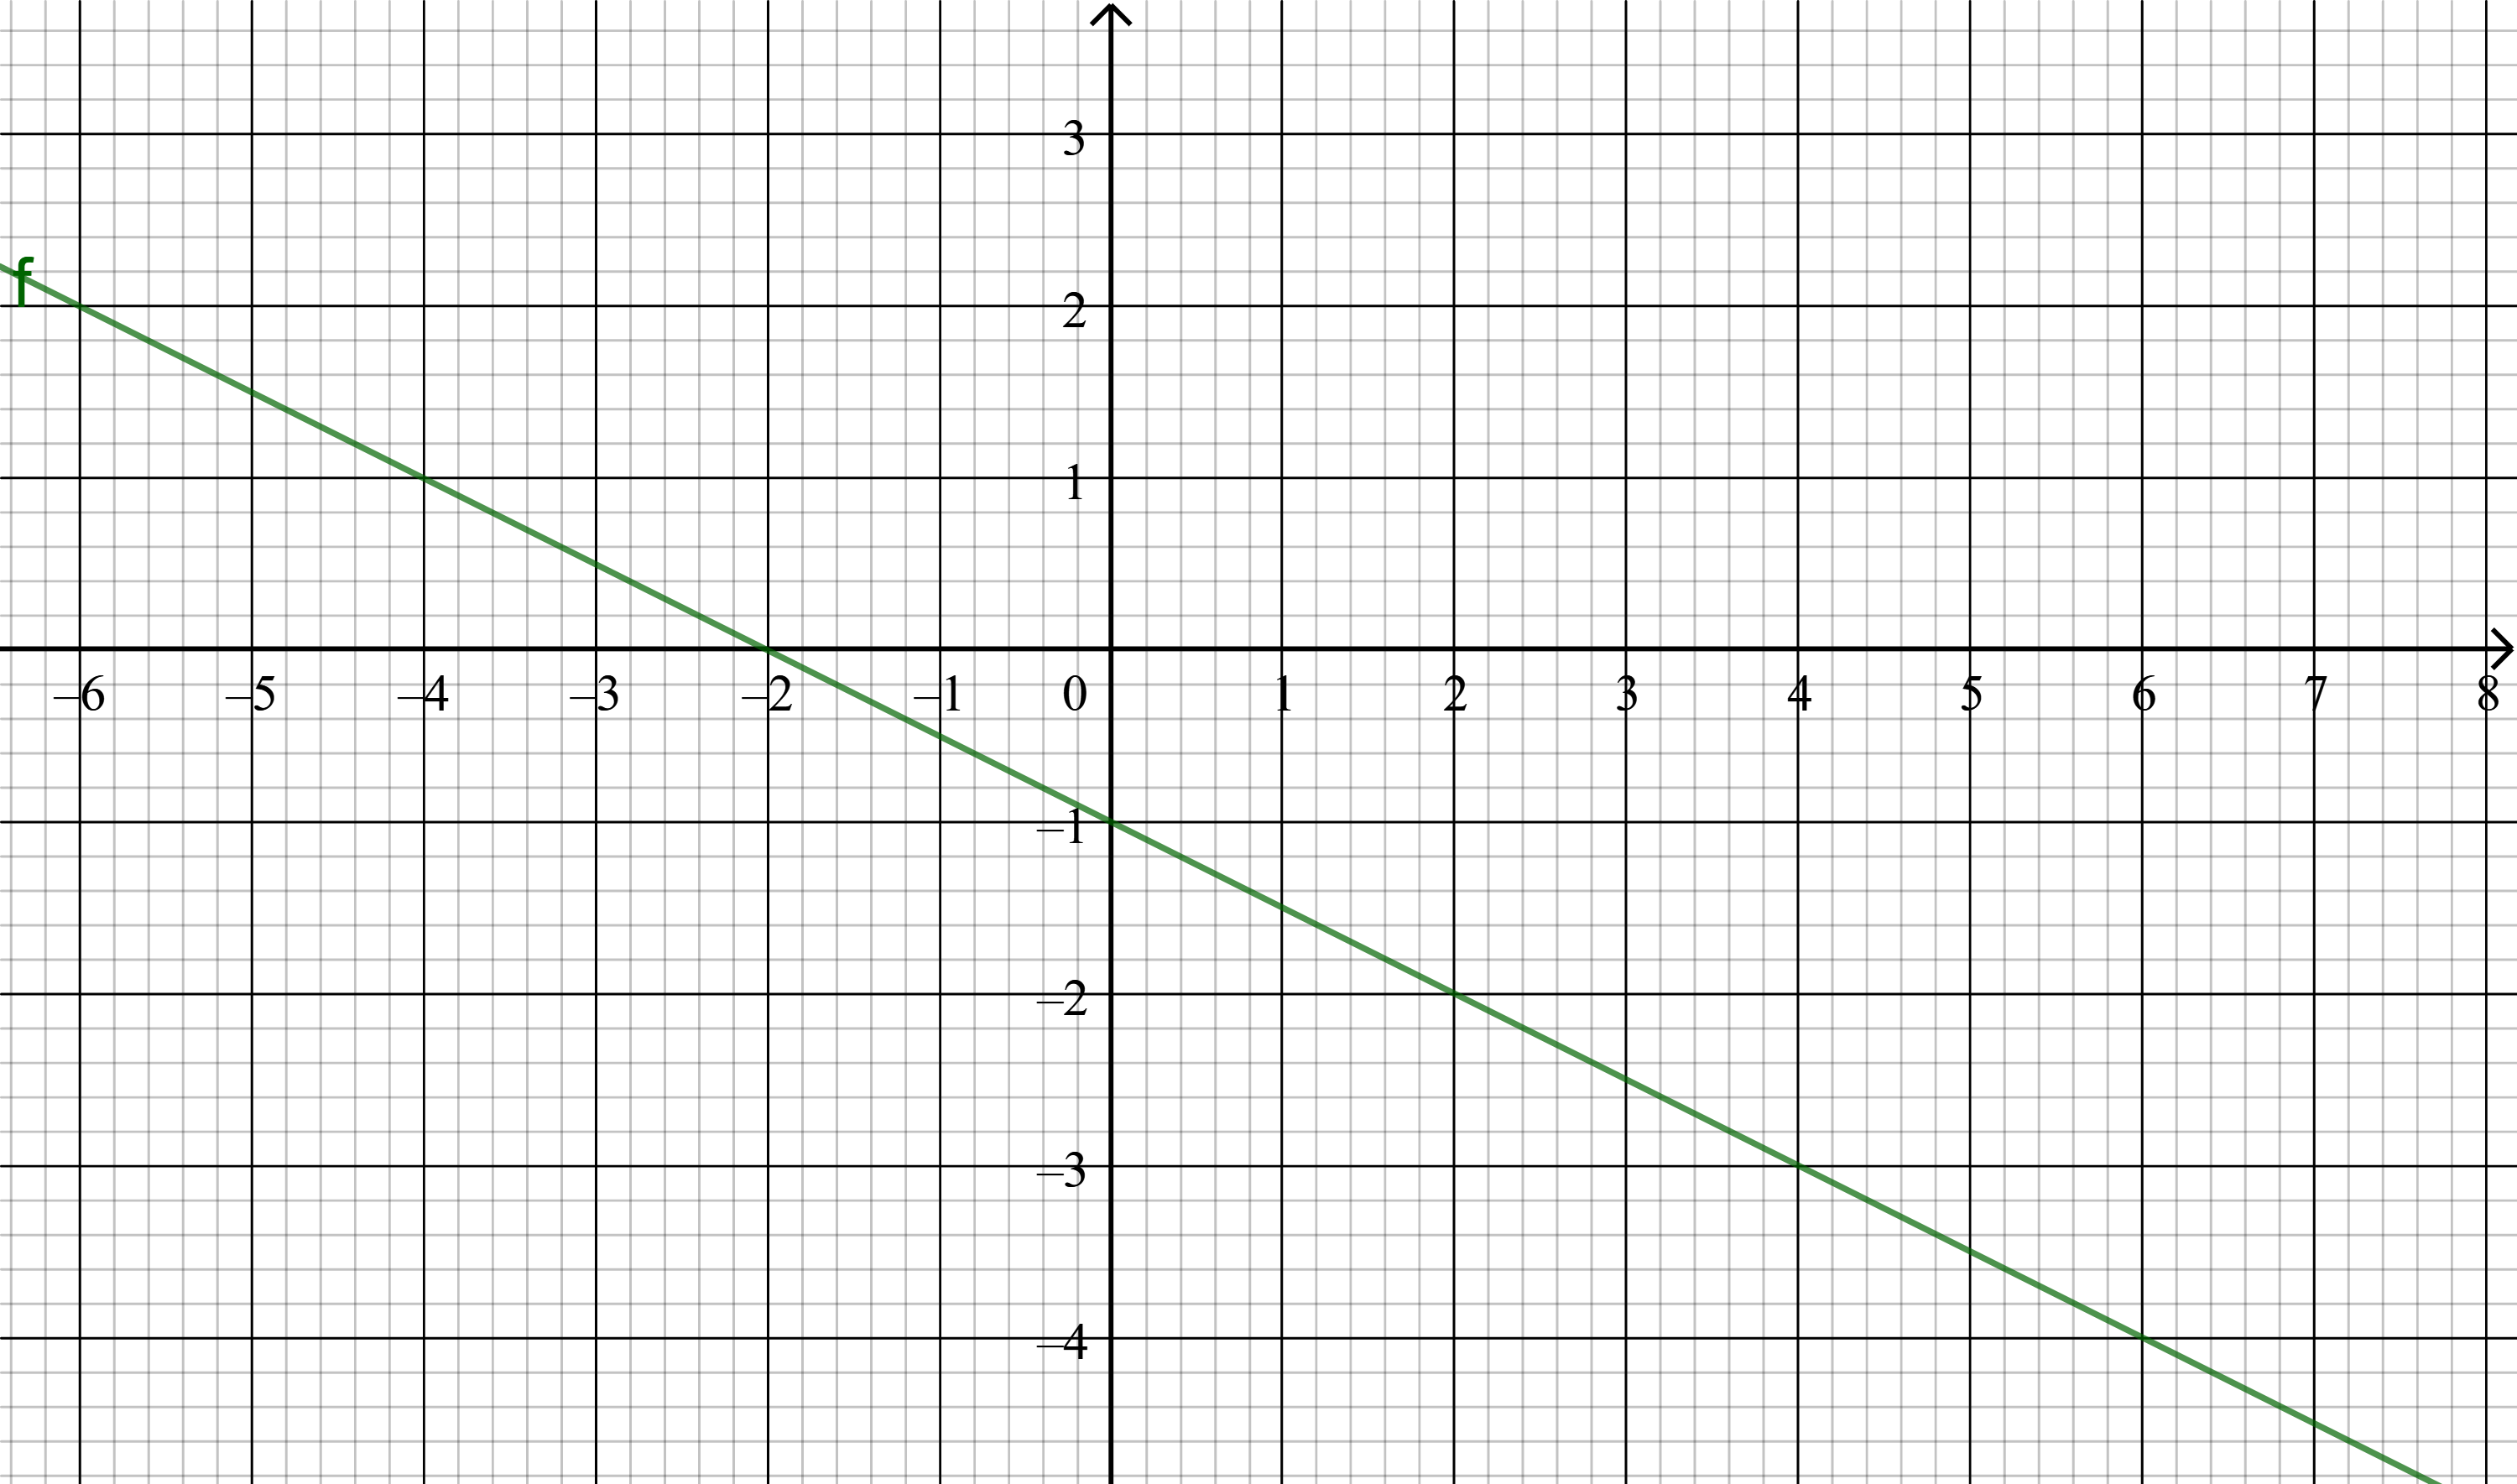
\includegraphics[width=0.5\textwidth]{pics/LinFunktion4}\\
         Bestimme die Funktionsgleichung von f.
    }
    \solution{$f(x)=-\frac{1}{2}x-1$
    }
\end{Add}

\begin{Add}{MaI}{basal1.2}{Lineares,Funktionen}{schwieriger}
    \question{
        Gegeben ist der Graph der Funktion f. \\
        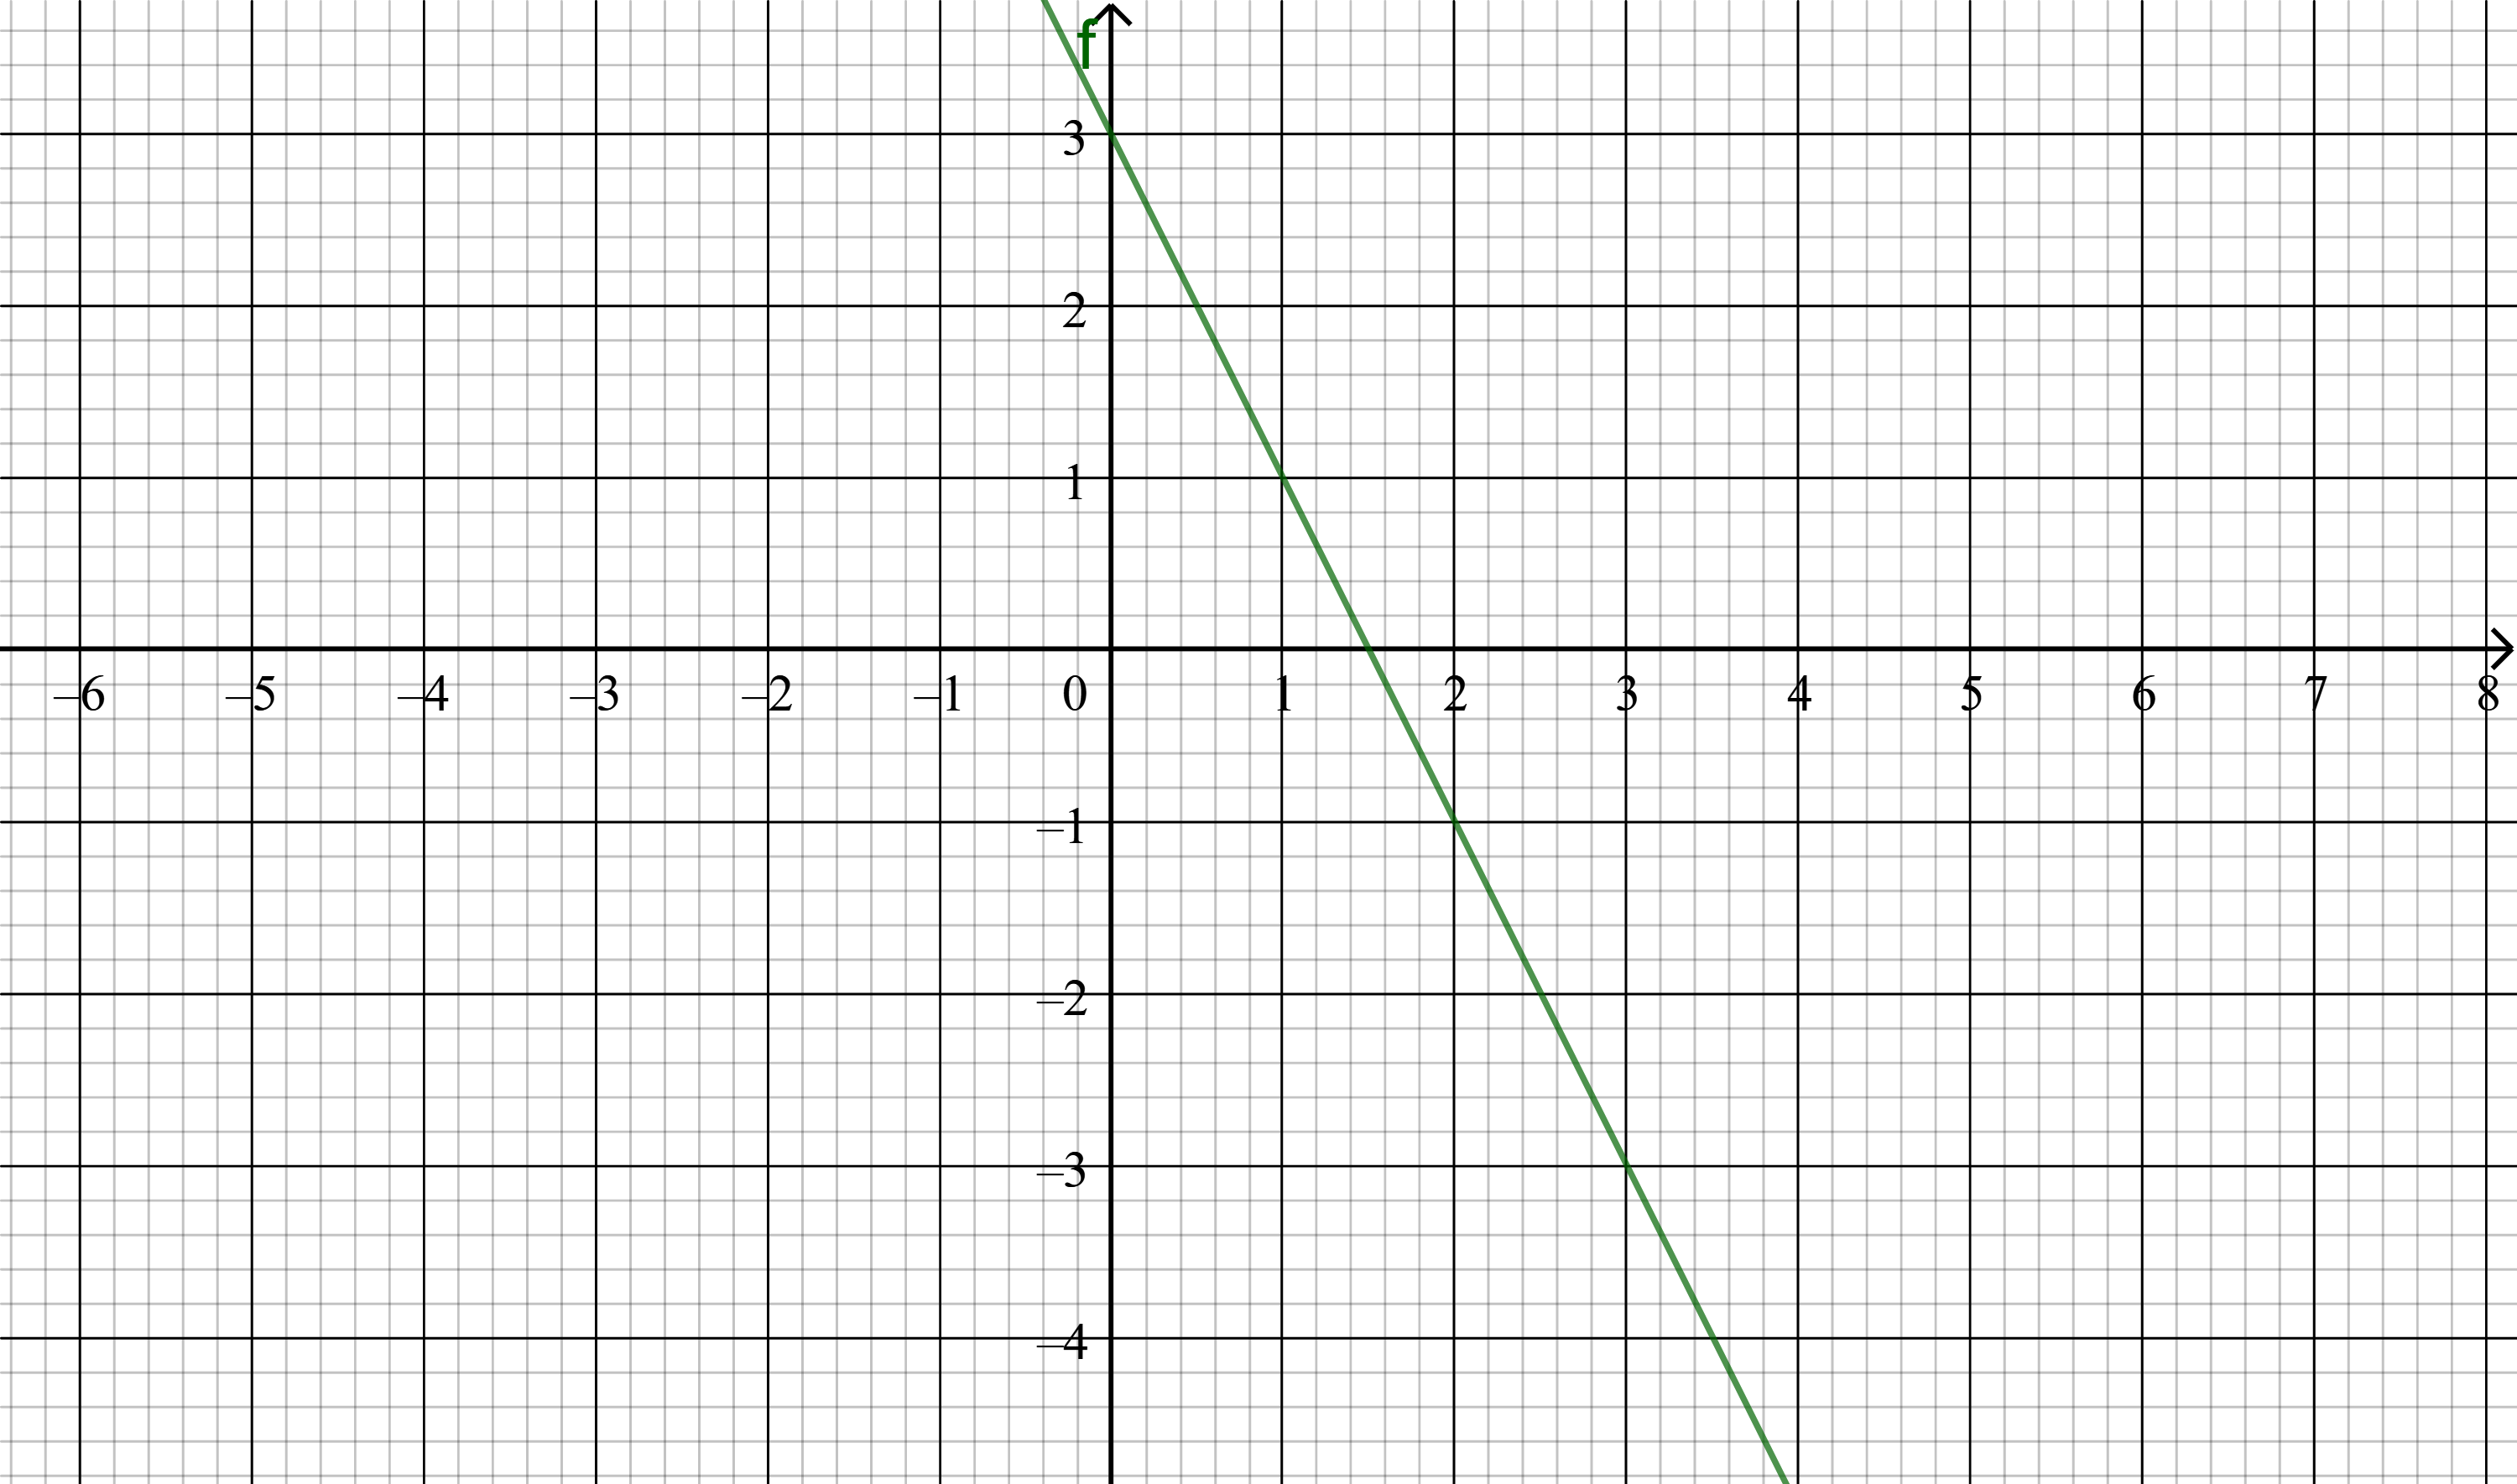
\includegraphics[width=0.5\textwidth]{pics/LinFunktion5}\\
         Bestimme die Funktionsgleichung von f.
    }
    \solution{$f(x)=-2x+3$}
\end{Add}

\begin{Add}{NeO}{basal0}{Mathematisieren}{schwieriger}
    \question{Formuliere sprachlich: \\
    \begin{tabular}{rrr}  $x \leq 2$ & $x \geq 2$ & $x \neq 2$ \end{tabular}}
    \solution{\begin{tabular}{rrr} $x$ ist höchstens 2 & $x$ ist mindestens 2 & $x$ ist ungleich 2 \end{tabular}}
\end{Add}

\begin{Add}{NeO}{basal0}{Mathematisieren}{schwieriger}
    \question{Sind die beiden Terme $a+((b \cdot c)-3)$ und $-3+a+bc$ äquivalent?}
    \solution{Ja}
\end{Add}

\begin{Add}{NeO}{basal0}{Grundoperationen,Sachrechnen}{einfach}
    \question{Runde 1.235 auf drei Werteziffern}
    \solution{1.24}
\end{Add}

\begin{Add}{NeO}{basal0}{Grundoperationen,Sachrechnen}{schwieriger}
    \question{Runde 12 auf eine Werteziffer}
    \solution{10}
\end{Add}


\begin{Add}{ScM}{basal1.1}{Mathematisieren}{schwieriger}
    \question{
    Beschreibe alle grünen Flächen mit einem Term (z.B. ist die Fläche des oranges Quadrats oben links $a^2$.) und vereinfache diesen soweit als möglich.
    \begin{center}
     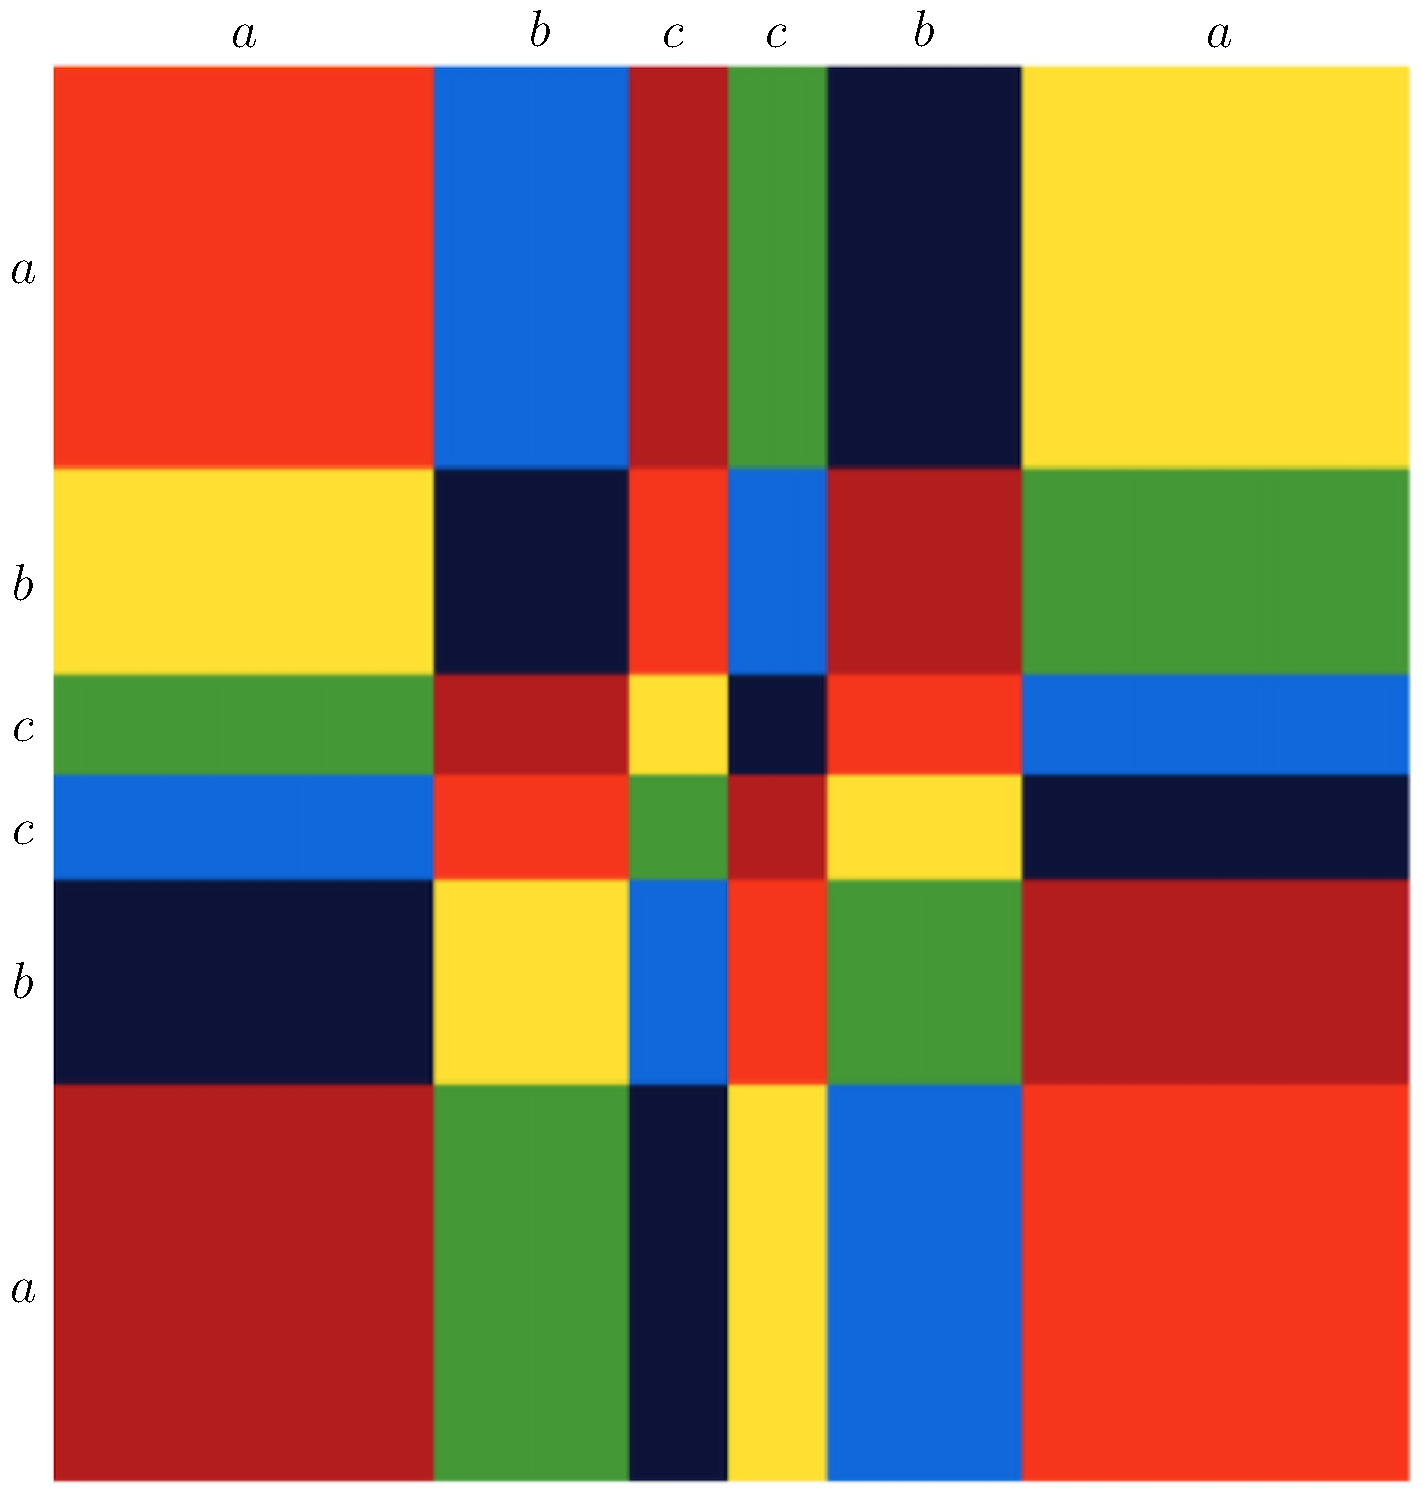
\includegraphics[width=0.3\textwidth]{pics/Lohse2}
     \end{center}
    }
    \solution{
    $2ab+2ac+b^2+c^2$
    }
\end{Add}

\begin{Add}{ScM}{basal0}{Sachrechnen}{schwieriger}
    \question{In einem Laden siehst Du ein T-Shirt. Der Preis von 49.50\,Fr ist nun um 10\,\% reduziert. Wie viel kostet das T-Shirt noch?}
    \solution{44.55\,Fr}
\end{Add}

\begin{Add}{ScM}{basal0}{Arithmetik}{einfach}
    \question{Schreibe die folgenden Zahlen in wissenschaftlicher Schreibweise:
    \begin{itemize}
        \item[a)] 10000
        \item[b)] 4'500'000
    \end{itemize}}
    \solution{a) \; $1\cdot 10^{4}$ \hspace{1cm} b) \; $4.5\cdot 10^{6}$ }
\end{Add}

\begin{Add}{ScM}{basal1.1}{Arithmetik}{schwieriger}
    \question{Schreibe die folgenden Zahlen in wissenschaftlicher Schreibweise:
    \begin{itemize}
        \item[a)] 0.000'001
        \item[b)] 0.01324
    \end{itemize}}
    \solution{a) \; $1\cdot 10^{-6}$ \hspace{1cm} b) \; $1.324\cdot 10^{-2}$ }
\end{Add}

\begin{Add}{ScM}{basal1.1}{Arithmetik}{schwieriger}
    \question{Schreibe die folgenden Zahlen in wissenschaftlicher Schreibweise und auf drei wesentliche Ziffern gerundet:
    \begin{itemize}
        \item[a)] 347601
        \item[b)] 0.002304
    \end{itemize}}
    \solution{a) \; $3.48\cdot 10^{5}$ \hspace{1cm} b) \; $2.30\cdot 10^{-3}$ }
\end{Add}

\begin{Add}{ScM}{basal0}{Arithmetik}{einfach}
    \question{Berechne (ohne Taschenrechner): $\sqrt{121}$}
    \solution{11}
\end{Add}

\begin{Add}{ScM}{basal0}{Arithmetik}{einfach}
    \question{Berechne (ohne Taschenrechner): $\sqrt{81}$}
    \solution{9}
\end{Add}

\begin{Add}{ScM}{basal1.1}{Arithmetik}{schwieriger}
    \question{Berechne und gib das Resultat als Dezimalbruch an (ohne Taschenrechner): $\sqrt{\dfrac{9}{25}}$}
    \solution{0.6}
\end{Add}

\begin{Add}{ScM}{basal1.1}{Arithmetik}{einfach}
    \question{Wahr oder falsch? $$\sqrt{3}+\sqrt{4}=\sqrt{7}$$}
    \solution{falsch}
\end{Add}

\begin{Add}{ScM}{basal1.1}{Algebra}{einfach}
    \question{Vereinfache: $$a^3 \cdot a^4 = $$}
    \solution{$a^7$}
\end{Add}

\begin{Add}{ScM}{basal1.1}{Algebra}{einfach}
    \question{Vereinfache: $$a^{10} / a^2 = $$}
    \solution{$a^8$}
\end{Add}

\begin{Add}{ScM}{basal1.1}{Arithmetik}{schwieriger}
    \question{Wahr oder falsch? $$\sqrt{5}\cdot \sqrt{3}=\sqrt{15}$$}
    \solution{wahr}
\end{Add}

\begin{Add}{ScM}{basal0}{Gleichungen,Lineares}{schwieriger}
    \question{Für welche $x$ ist die  Gleichung $17 + x = 2x - 1$ wahr? }
    \solution{$x=18$}
\end{Add}

\begin{Add}{ScM}{basal0}{Gleichungen,Lineares}{schwieriger}
    \question{Löse nach $x$ auf: $$7x-(4x-5) = 29$$ }
    \solution{$x=8$}
\end{Add}

\begin{Add}{ScM}{basal0}{Gleichungen,Lineares}{schwieriger}
    \question{Löse nach $x$ auf: $$13+4(6x-5)=5(5x+2)$$ }
    \solution{$x=-17$}
\end{Add}

\begin{Add}{ScM}{basal0}{Gleichungen,Lineares}{schwieriger}
    \question{Löse nach $x$ auf: $$4(5x-6)-7 = 4-5(6x-7)$$}
    \solution{$x=\dfrac{7}{5}=1.4$}
\end{Add}

\begin{Add}{ScM}{basal1.1}{Gleichungen}{schwieriger}
    \question{Bestimme $x$: $$x^2 + 17=x(x-11)-49$$ }
    \solution{$x=-6$}
\end{Add}

\begin{Add}{ScM}{basal1.1}{Gleichungen}{schwieriger}
    \question{Löse nach $x$ auf: $$(x-3)(2x-5)+4(2-x)+12=2(1-x)^2$$ }
    \solution{$x=3$}
\end{Add}

\begin{Add}{ScM}{basal1.1}{Algebra}{schwieriger}
\question{Vereinfache den Term  $$4x - 2y + 3x + 5y + 7x - y - 8x + 4y$$ soweit als möglich.  }
    \solution{$6x + 6y$ \; bzw. \; $6(x+y)$}
\end{Add}

\begin{Add}{ScM}{basal1.1}{Algebra}{schwieriger}
    \question{Berechne den Wert des Terms $3a^2 - 7a + 11$ für:
    \begin{itemize}
        \item[a)] $a=3$
        \item[b)] $a=-2$
    \end{itemize}}
    \solution{a) \; $17$ \hspace{1cm} b) \; $37$ }
\end{Add}


\begin{Add}{GiD}{basal0}{Arithmetik}{einfach}
    \question
    {Vereinfache den gewöhnlichen Bruch so weit wie möglich.
        $$\frac{5}{6}+\frac{2}{5}=\;?$$
        $$\frac{5}{6}\cdot\frac{2}{5}=\;?$$
    }
    \solution{
        $\frac{37}{30}=1\frac{7}{30} ; \frac{1}{3}$
    }
\end{Add}

\begin{Add}{GiD}{basal0}{Grundoperationen}{einfach}
    \question {Vereinfache so weit wie möglich.
    \begin{itemize}
        \item[a)] \ $6+5 \cdot 7-4=\;?$
        \item[b)] \ $(6+5) \cdot  7-4=\;?$
    \end{itemize}}
    \solution{a) \; $37$  \hspace{1cm} b) \; $73$}
\end{Add}

\begin{Add}{GiD}{basal0}{Geometrie}{einfach}
    \question {Ein Rechteck hat eine Länge von 8,75 cm und sein Umfang misst 27,9 cm. Berechne seine Breite und seinen Flächeninhalt.}
    \solution{$b = 5,2 cm \hspace{1cm}und \hspace{1cm}A = 45,5 cm^2$}
\end{Add}

\begin{Add}{GiD}{basal0}{Grundoperationen}{einfach}
    \question {Rechne Schritt für Schritt aus.$$(19-6 \cdot 3)+(5-80:20)-(3 \cdot 12-35)+((6+3)-(27:3))=$$}
    \solution{$1$}
\end{Add}

\begin{Add}{GiD}{basal0}{Geometrie}{einfach}
    \question {Ein Kreis hat einen Durchmesser von 11 cm. Berechne seinen Umfang u und seinen Flächeninhalt A.}
    \solution{$u=34,54 cm \hspace{1cm} A = 94,985 cm^2$}
\end{Add}

\begin{Add}{JcD}{basal0}{Arithmetik,Grundoperationen}{schwieriger}
    \question {Welche Zahl ist grösser?
    
        $$-3^2 \text{\ oder \ } (-3)^2$$    
    }
    \solution{$(-3)^2$}
\end{Add}

\begin{Add}{JcD}{basal0}{Koordinatensystem}{schwieriger}
    \question {Spiegele den Punkt $P (-1/4)$ am Ursprung.}
    \solution{$P'(1/-4)$}
\end{Add}

\begin{Add}{JcD}{basal0}{Grundoperationen,Algebra}{schwieriger}
    \question {Vereinfache so weit wie möglich.
    
    $$a^4-(a^3+2)+a^4-(4-a^3)$$}
    \solution{$2a^4-6$}
\end{Add}

\begin{Add}{JcD}{basal0}{Geometrie}{einfach}
    \question {Ein Quadrat hat den Flächeninhalt $A=16 cm^2$. 
    \\[2mm]
    Bestimme den Umfang.}
    \solution{$16 cm$}
\end{Add}

\begin{Add}{JcD}{basal1.1}{Funktionen,Lineares}{schwieriger}
    \question {Gegeben ist die Funktion $f(x)=-2x+5$.
    \\[2mm]
    Welcher Funktionswert ist größer: $f(-2)$ \ oder \ $f(2)$?}
    \solution{$f(-2)=9>f(2)=1$}
\end{Add}

\begin{Add}{JcD}{basal0}{Arithmetik,Grundoperationen}{einfach}
    \question {Welche Zahl ist größer  $2^3$ \ oder \ $3^2$?}
    \solution{$3^2=9>2^3=8$}
\end{Add}

\begin{Add}{JcD}{basal0}{Arithmetik,Grundoperationen,Bruchterme}{schwieriger}
    \question {Berechne: $$\frac{4 \cdot 10^3}{2 \cdot 10^4}$$}
    \solution{$0.2$}
\end{Add}

\begin{Add}{JcD}{basal1.1}{Funktionen,Lineares}{einfach}
    \question {Liegt der Punkt $P(1/3)$ auf der Geraden $y=2x+3$ ?}
       \solution{nein}
\end{Add}

\begin{Add}{JcD}{basal1.1}{Funktionen,Lineares}{schwieriger}
    \question {Bestimme die Gleichung der Geraden, die durch die
    \\ Punkte $ A (11/5) $ und  $ B (3/-3)$ geht.}
    \solution{$y= x-6$}
\end{Add}

\begin{Add}{JcD}{basal1.1}{Gleichungen,Algebra}{einfach}
    \question {Löse: \ $4x+5=7-2x$}
    \solution{$x=\frac{1}{3}$}
\end{Add}

\begin{Add}{JcD}{basal1.1}{Arithmetik,Wurzelterme}{schwieriger}
    \question {Vereinfache: $(\sqrt{3}-2)\cdot (\sqrt {3}+4)$}
    \solution{$2\cdot\sqrt{3}-5$}
\end{Add}

\begin{Add}{JcD}{basal0}{Gleichungen,Algebra}{einfach}
    \question {Vereinfache: \ $3a-2(a+5)+2(3-a))$}
    \solution{$-a-4$}
\end{Add}

\begin{Add}{JcD}{basal1.1}{Bruchterme,Gleichungen,Algebra}{schwieriger}
    \question {Bestimme x: $$\frac{2}{x-5}-\frac{1}{3}=\frac{5}{6x-30}$$}
    \solution{$x=8.5$}
\end{Add}

\begin{Add}{JcD}{basal0}{Grundoperationen}{einfach}
    \question {Berechne: \ $(t^2)^3=$}
    \solution{$t^6$}
\end{Add}

\begin{Add}{JcD}{basal0}{Grundoperationen}{einfach}
    \question {Berechne: \ $t^2\cdot t^3=$}
    \solution{$t^5$}
\end{Add}

\begin{Add}{JcD}{basal1.1}{Quadratisches,Algebra}{schwieriger}
    \question {Die Gleichung ist falsch. Bestimme die zwei Fehler. \\[4 mm] $(b-5)^2=b^2-5b-25$}
    \solution{$(b-5)^2=b^2-10b+25$}
\end{Add}

\begin{Add}{JcD}{basal0}{Geometrie}{schwieriger}
    \question {In einem Dreieck sind zwei Winkel gleich gross und der dritte Winkel ist doppelt so gross, wie einer der beiden anderen Winkel. Wie gross sind die Winkel in dem Dreieck?}
    \solution{Die Winkel sind 45, 45 und 90 Grad}
\end{Add}

\begin{Add}{JcD}{basal1.1}{Funktionen,Lineares}{schwieriger}
    \question {Wo schneidet die Funktion $f(x)=-3x+9$ die x- und die y-Achse?}
    \solution{$x= 3$ und $y= 9$}
\end{Add}

\begin{Add}{JcD}{basal1.1}{Mathematisieren}{schwieriger}
    \question {Behauptung:  \\ Wenn man 5 durch eine Zahl dividiert, ist das Ergebnis immer kleiner als 5.
    \\ 
    \\ Zeige durch ein Gegenbeispiel, dass diese Aussage falsch ist.}
    \solution{$5/0.2 = 25$}
\end{Add}

\begin{Add}{JcD}{basal1.1}{Sachrechnen}{schwieriger}
    \question {Kann man in einen Becher, der 10 cm hoch ist und dessen kreisförmige Grundfläche einen Durchmesser $d = 10cm$ hat, einen Liter Flüssigkeit einfüllen?}
    \solution{nein:  $V = 0.785$ Liter}
\end{Add}

\begin{Add}{JcD}{basal0}{Sachrechnen,Geometrie}{schwieriger}
    \question {Wie viel $m^2$ misst die Fläche eines Rechtecks, das einen Umfang von $1.00 m$ hat und dessen eine Kante $30 cm$ lang ist.}
    \solution{$A = 0.06 m^2$}
\end{Add}

\begin{Add}{JcD}{basal1.1}{Quadratisches,Geometrie}{schwieriger}
    \question {In einem rechtwinkligen Dreieck ist die eine \\Kathete $a=4 cm$ und die Hypotenuse $c=5 cm$ lang.
    \\ Berechne den Flächeninhalt A des Dreiecks.}
    \solution{$A = 6 cm^2$}
\end{Add}

\begin{Add}{JcD}{basal0}{Grundoperationen,Bruchterme,Algebra}{schwieriger}
    \question {Vereinfache so weit wie möglich: \ $\frac{2a-4}{2a}$}
    \solution{$\frac{a-2}{a}$}
\end{Add}

\begin{Add}{JcD}{basal1.1}{Grundoperationen,Bruchterme,Algebra}{schwieriger}
    \question {Vereinfache so weit wie möglich: \ $\frac{b^2-ba}{ab-a^2}$}
    \solution{$\frac{b}{a}$}
\end{Add}

\begin{Add}{JcD}{basal1.1}{Mathematisieren,Grundoperationen}{schwieriger}
    \question {Wie gross ist ein Viertel von einem Drittel?
    \\[4mm] Wie gross ist ein Drittel von einem Viertel?}    \solution{in beiden Fällen ein Zwölftel}
\end{Add}

\begin{Add}{GiD}{basal0}{Mathematisieren}{schwieriger}
    \question {Für die Fahrt von A nach B ist ein Zug mit 70 km/h unterwegs und kommt nach 45 Minuten am Ziel an. Wie lange braucht der Zug für die Rückfahrt, wenn er mit 84 km/h fahren kann? (Gib das Ergebnis in Minuten und Sekunden an.)}
    \solution{$37$ $Minuten$ $30$ $Sekunden$}
\end{Add}

\begin{Add}{GiD}{basal0}{Arithmetik}{einfach}
    \question {Verwandle die gemischte Zahl 5$\frac{6}{7}$ in den gleichwertigen unechten Bruch.}
    \solution{$\frac{41}{7}$}
\end{Add}

\begin{Add}{GiD}{basal0}{Geometrie}{schwieriger}
    \question {Berechne beim regelmässigen 15-Eck die Grösse ...
    \begin{itemize}
        \item[a)] \ $der$ $Summe$ $der$ $Innenwinkel;$
        \item[b)] \ $eines$ $Innenwinkels;$
        \item[b)] \ $eines$ $Mittelpunktswinkels.$
    \end{itemize}}
    \solution{a) \; $2'340\; Winkelgrad$  \hspace{1cm} b) \; $156\; Winkelgrad$ \hspace{1cm} c) \; $24\; Winkelgrad$}
\end{Add}

\begin{Add}{GiD}{basal0}{Geometrie}{schwieriger}
    \question {Ein Quadrat mit einer Seitenlänge von 6,4 cm ist flächengleich einem Rechteck, das eine Länge von 8 cm hat. Berechne den Umfang des Rechtecks.}
    \solution{$Umfang = 26,24$ $cm$ $(Breite =5,12$ $cm)$}
\end{Add}

\begin{Add}{GiD}{basal0}{Mathematisieren}{einfach}
    \question {Laura hat 19,60 Franken im Portemonnaie: Viermal so viele Zwanzigrappenstücke wie Zweifrankenstücke. Wie viele Stücke hat sie von jeder Münzsorte?}
    \solution{Laura hat 28 Zwanzigrappenstücke und 7 Zweifrankenstücke.}
\end{Add}

\end{document}